%%%%%%%%%%%%%%%%%%%%%%%%%%%%%%
\chapter{Background}
\label{chap:background}

This chapter explains the fundamental theory and mathematics that went into the development of WARP.  It covers nuclear physics, nuclear reactor analysis, and the kinematics involved in neutron transport.  Next, the mathematics behind the governing equations is discussed, the Monte Carlo solution method explained, and how the required probability distributions are sampled is detailed.  After the physics and mathematics sections, the computer hardware is discussed as is the OptiX ray tracing framework, which is the major library used in WARP.  The chapter concludes with an overview of the previous research of Monte Carlo neutron transport on GPUs and how WARP fits into the landscape.

%%%%%%%%%%%%%%%%%%%%%%%%%%%%%%
\section{Nuclear Reactor Analysis}
\label{sec:analysis}

Nuclear reactors generate electricity from the heat produced by fissions induced in heavy nuclei.  Fissions are induced in nuclear reactor cores by a free neutron population present in the core, and this free neutron population is self-sustaining if the core is maintained within certain property ranges.  The neutron density in the core is much smaller than the nuclei density and it can change much more quickly.  Reactor power is directly proportional to the neutron flux, which is derived from the neutron density, and thus can change as quickly as the flux.  Therefore, to know a core's most basic state, one must know the neutron distribution.  Knowing how reactor power will change given changes in the environment means knowing how the neutron distribution will respond to the changes.  Accurately solving the neutron transport equation is essential for characterizing reactor behavior. 

When a uranium (or other fissile heavy metal) nucleus fissions, two or more neutrons are released.  If, on average, exactly one of these neutrons goes on to induce another fission, the system in which the fissions are occurring is \emph{critical}, or able to maintain a constant neutron population and fission reaction rate (and correspondingly constant power) without any external neutron sources.  This is a stable fission chain reaction.  The fissile nucleus rarely splits evenly, and the spectrum of lighter isotopes that are created by fission are called \emph{fission products} \cite{duderstadt}.  Fission products accumulate in the fuel material and can inhibit the fission chain reaction through absorption when the reach a high enough concentration.
% what fission products are

A \emph{fissionable} isotope is one that has a non-zero fission cross section, i.e. it there is a probability that it will fission if it absorbs a neutron.  A \emph{fissile} isotope is one that can be induced to fission by absorbing a neutron at any energy.  Some isotopes, like $^{235}$U, can absorb a neutron a very low energies and fission.  This is because the energy imparted to the nucleus through the absorption reaction is enough to destabilize to the point where it splits \cite{duderstadt}.  For some isotopes, like $^{238}$U, absorbing a low-energy neutron does not impart enough energy to the nucleus to induce fission.  It only fissions when a high-energy neutron is absorbed and the neutron brings additional energy with it to destabilize the nucleus sufficiently for fission to occur.  Therefore, $^{238}$U is fissionable, but not fissile.  $^{238}$U is also considered a \emph{fertile} isotope since when it captures a neutron, it become	s $^{239}$U which decays to $^{239}$Np and then to $^{239}$Pu, which is fissile.  Absorbing a neutron and only producing no secondary particles other than a gamma rays is called ``capture'' since the neutron is added to the nucleus of the previous isotope.  Fertile isotopes are those that decay to fissile isotopes after capturing a neutron \cite{duderstadt}.
%define fissile/fertile here, you might want to mention why nu exists at very low energies since this seems inconsistent.

The \emph{effective multiplication factor}, $k_\mathrm{eff}$, is the ratio of the number of neutrons in subsequent neutron generations. It is an integral quantity, and describes how many secondary neutrons are induced by an an average neutron in a core.  In other words, describes the growth rate of the neutron population in terms of generations.  If $k_\mathrm{eff}=1$, then subsequent neutron generations are exactly the same size and the core is critical.  If it is below 1, subsequent neutron generation are smaller and the core is subcritical.  If $k_\mathrm{eff}$ is greater than 1, subsequent generations are larger and the core is supercritical.  The effective multiplication factor can also describe the time rate of change of the neutron population if the average neutron lifetime is known.  The multiplication factor is an important quantity in characterizing nuclear reactor behavior because the core power is directly proportional to the neutron population, and the multiplication factor therefore dictates the time rate of change of its power.

\begin{figure}[h!]
  \centering
    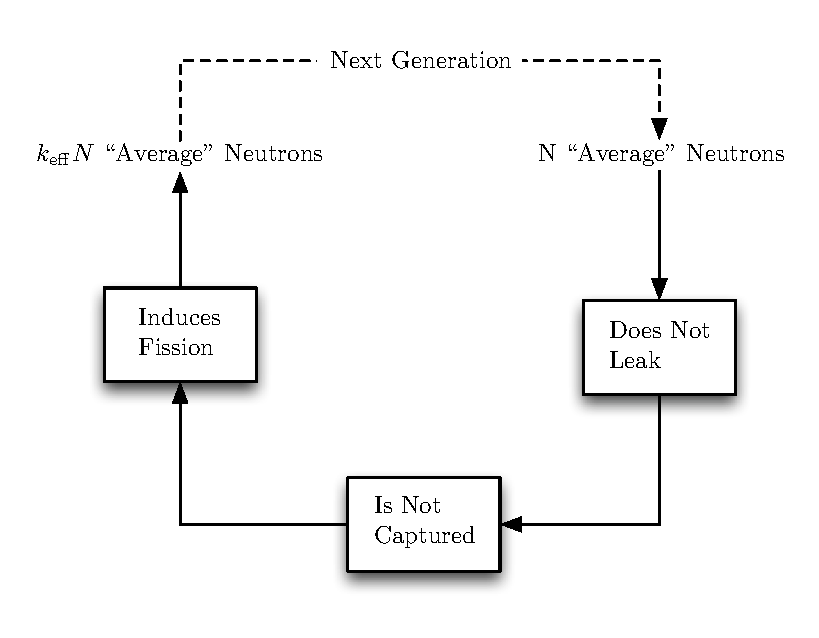
\includegraphics[width=0.8\textwidth]{graphics/k_chain.eps}
     \caption{The fission chain reaction and its relation to the multiplication factor. \label{k_chain}}
\end{figure}

The most common type of commercial reactor is an oxide-fueled light water reactor \cite{reactor_numbers}.   These reactors use ceramic fuel elements made of uranium oxide, UO$_2$, due to its high melting point.  They are also cooled and moderated with light water, which is water containing predominately $^1$H with trace amounts of $^2$H.  In the nuclear engineering lexicon, ``moderator'' means a material that reduces neutron energies to thermal levels \cite{duderstadt}.  The most effective moderators are light nuclei, like hydrogen, since they have a mass similar to that of a neutron and an elastic scattering reaction can transfer a large amount of the neutron's energy to the nucleus.  Light water reactors, or LWRs, are called ``thermal'' as well, since their mode of operation relies on the neutrons' energies being at thermal levels.  ``Fast'' rectors, on the other hand, operate with high energy neutrons, and want to avoid moderating them.  For this reason, oxide fuel and water are typically not used in fast reactors, since they include light nuclei \cite{duderstadt}.
%describe typical fuel compositions. done.

%I SUGGEST YOU WILL DESCRIBE ALL THE PHENOMENA THE FISSION-BORN NEUTRON CAN UNDERGO -- AS THE M.C. CODE NEEDS TO SIMULATE THEM ALL, BUT DO NOT DEFINE THE SIX FACTORS. IT MAY BE BEST (BUT NOT NECESSARY) TO DO SO FOR A FAST REACTOR, A THERMAL REACTOR, A SUBCRITICAL SYSTEM SUBJECTED TO AN EXTERNAL NEUTRON SOURCE  AND A NON-MULTIPLYING SYSTEM SUBJECTED TO AN EXTERNAL SOURCE. -- YOU ARE ADDRESSING ALL THESE SYSTEMS IN YOUR BENCHMARKS

%describe the need to model all reactions here, go into the dominant types for fast/thermal

Many factors influence the neutron population, and therefore must be incorporated into the solution method.  The neutron population has strong feedback mechanisms from the materials present in the core.  Each isotope in the may undergo several different interactions with neutrons, and these reaction probabilities may have very strong dependence on the incoming neutron energy.  Using the Monte Carlo method to approximate solutions to the neutron transport equation requires all of the neutron interactions to be explicitly modeled.  The core geometry also effects the neutron distribution, since it describes the spatial extent of the core materials.   The Monte Carlo method tracks neutrons as they move through the core materials, sampling the reactions they can undergo along the way.   These reactions dictate fission chain reaction and maintain the core's effective multiplication factor.  Tracking them allows the estimation of detailed reaction rates in the core, and allows engineers to better understand reactor behavior and design reactors to specifications.  Since a neutron's every interaction to be explicitly modeled, the next section will discuss all the possible reaction types a neutron can undergo when it collides with a nucleus and how interaction probabilities are classified and quantified.


%\subsection{Point Kinetics, Multiplication Factor}

%The most important parameter of a nuclear reactor is its effective multiplication factor, $k_\mathrm{eff}$, .  All of the work put into reactor analysis and solving the neutron transport equations can usually be condensed into the effective multiplication factor.    

%The effective multiplication factor can also describe the time rate of change of the neutron population if the average neutron lifetime is known.  If a reactor is treated as a point (which means it has no spatial \emph{dependence}, not that it has no spatial \emph{extent}), the rate of change of its neutron population can be described with the differential equation shown in \eqref{point_kin1}, where $N(t)$ is the neutron population at time $t$ and $l_p$ is the average neutron lifetime \cite{duderstadt}.  The expression on the left side is the neutron population after a mean neutron lifetime, which is equal to the multiplication factor multiplied by the initial neutron population.  The expression on the left hand side can be Taylor expanded to first order by the middle expression.  Rearranging this equation yields the ODE shown in  \eqref{point_kin2} \cite{duderstadt}.

%\begin{equation}
%\label{point_kin1}
%N(t+l_p) \simeq N(t)+l_p \frac{dN(t)}{dt} = k_\mathrm{eff} N(t) 
%\end{equation}
%
%\begin{equation}
%\label{point_kin2}
%\frac{dN(t)}{dt} \simeq \frac{k_\mathrm{eff} -1}{l_p}N(t)
%\end{equation}

%The solution to this equation is show in \eqref{reactor_period}, where $T$ is the reactor period and is defined as... \cite{duderstadt}.  The neutron lifetime is usually treated as constant since it largely depends on the materials present in the reactor, which change very slowly compared to the neutron population. Thus, the only parameter that influences the reaction period, $T$, is $k_\mathrm{eff}$.  This does not mean that the mean neutron lifetime is not important, but rather that the only readily-changeable value in the reactor period expression is the multiplication factor.  The mean neutron lifetime, however, affects how \emph{fast} changes occur in the neutron population, which is of huge consequence in reactor control \cite{duderstadt}.  

%When the multiplication factor is unity, the reactor period is infinity, implying that the neutron population is in a steady state.  When it is less than one, the period is negative, implying that the neutron population will decrease.  The converse it true when it is positive.  Then the period is positive and the neutron population increases with time.

%\begin{equation}
%\label{reactor_period}
%\begin{split}
%N(t) &= N_0 \exp \left( \frac{t}{T} \right) \\
%T &= \frac{l_p}{k_\mathrm{eff} -1}
%\end{split}
%\end{equation}
%
%\subsection{Six Factor Formula}

%The multiplication factor is the most important parameter in a nuclear reactor because it dictates the time rate of change of its power.  It is a global number, and a lot of physics is integrated into it.   The reaction cross sections, the naming of which is discussed in the next section, describe the probabilities of neutron reactions occurring as a function of energy.  There are many individual reactions, but from a high level and speaking in broad terms, there are six probabilities that can influence the multiplication factor \cite{duderstadt}: 
%\begin{itemize}
% \item the thermal reproduction factor, $\eta$, or the average number of neutrons produced per neutron absorbed in the fuel;
% \item the thermal utilization factor, $f$, or the probability that an absorbed thermal neutron was absorbed by a fissile nuclide;
% \item the resonance escape probability, $p$, or the probability that neutrons are not captured in resonances as they scatter down from high energy to low energy;
% \item the fast fission factor, $\epsilon$, or the ratio of total fission neutrons (including high-energy fissions) to those born from thermal fissions;
% \item the fast non-leakage probability, $P_\mathrm{FNL}$, or the probability that high-energy neutrons will not leak out of the system; and
% \item the thermal non-leakage probability, $P_\mathrm{TNL}$, or the probability that low-energy neutrons will not leak out of the system.	
%\end{itemize}

%Multiplying all these factors together yields the number of neutrons born from fission given a single entering neutron, i.e. the multiplication factor.  This formula, known as the ``six factor formula,'' is shown in \eqref{six_ff_eq} \cite{duderstadt}.  Many physics factors go into each of the formula's factors, like geometrical configuration, cross section energy dependence, material composition, and scattering kinematics, et cetera.  A graphical interpretation of the six factor formula is shown in Figure \ref{six_ff_chain}.

%\begin{equation}
%\label{six_ff_eq}
%k_\mathrm{eff}  = \eta f p  \epsilon P_\mathrm{FNL} P_\mathrm{TNL}
%\end{equation}
%
%
%\begin{figure}[h!]
%  \centering
%    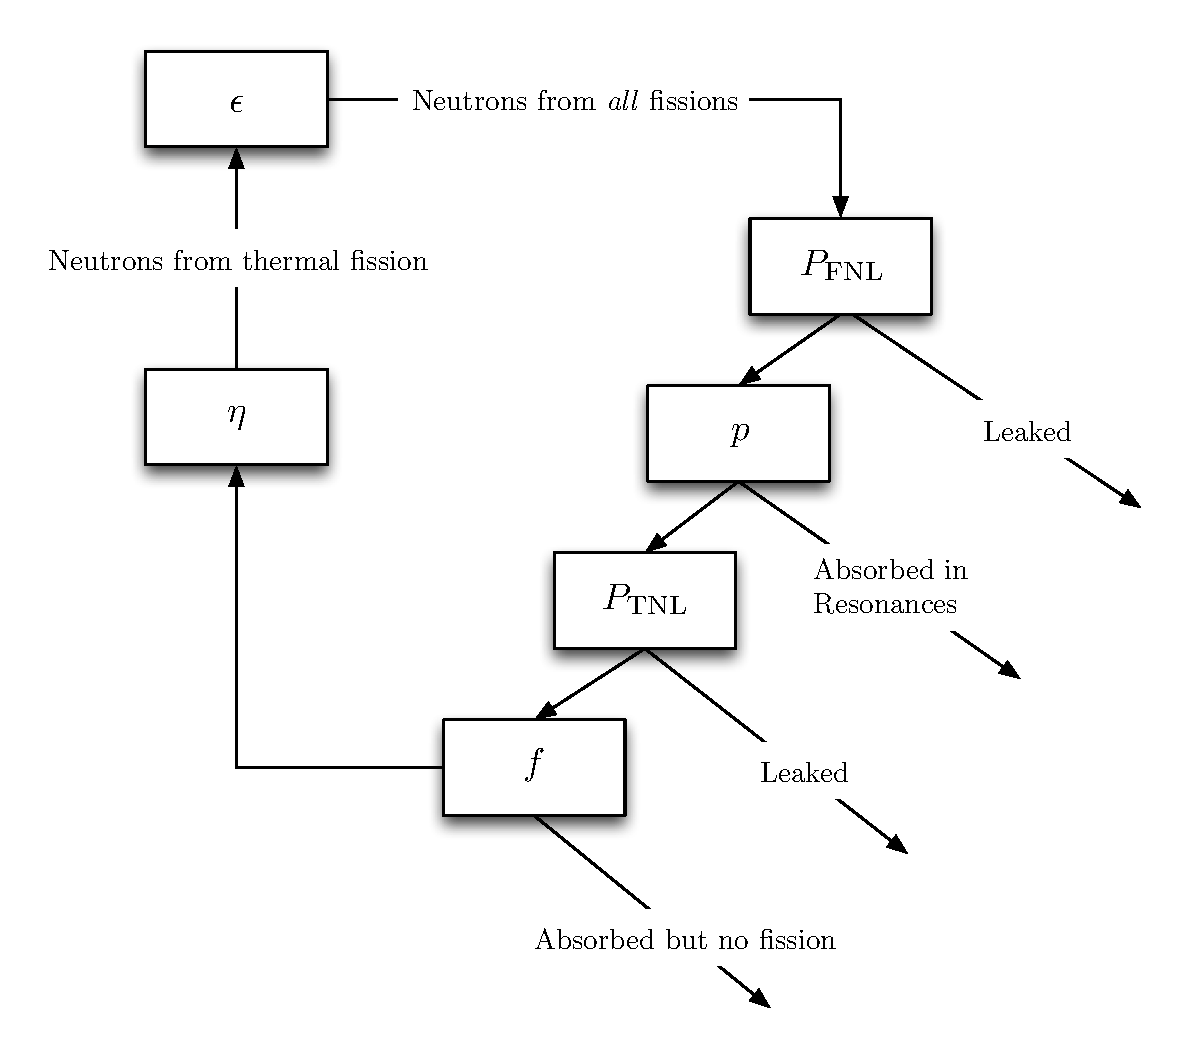
\includegraphics[width=0.8\textwidth]{graphics/six_ff.eps}
%     \caption{The reaction chain represented by probabilities in the six factor formula. \label{six_ff_chain}}
%\end{figure}
%
%The six factor formula describes what happens to the average neutron. An individual neutron history could be simulated by sampling the constant probabilities that the factors represent.  After a large group of these histories is simulated, they can be averaged to determine the multiplication factor.  This is the basic idea of Monte Carlo neutron transport.  The results are trivial in this case, since there is no dimensionally in the problem, the probabilities are constant, and the multiplication factor can be found analytically.  More broadly, though, the six factor formula is way to think about the process without complicating it with dimensionality.


%%%%%%%%%%%%%%%%%%%%%%%%%%%%%%
\section{Nuclear Interactions}
\label{subsec:interactions}

The core of a Monte Carlo simulation is explicitly modeling the individual interactions the neutron undergoes as it moves through matter.  At the highest level, these reactions can be broken down into two broad categories - scattering and absorption.  Scattering reactions are when a neutron ``bounces off'' a nucleus.  They change a neutron's direction and energy, but do not terminate its progression through materials.  Absorption reactions are when the neutron becomes part of the nucleus.  This state of a nucleus plus the incoming free neutron is called a ``compound nucleus.''  The neutron does not continue in a free state, and its progress through the material is ended.

Scattering reactions can be further broken down into elastic and inelastic types.  Elastic reactions are those where both momentum and kinetic energy are conserved, i.e. ones where any energy the neutron loses is given to the target nucleus.  Inelastic reactions are those that conserve momentum but do not conserve kinetic energy, i.e. ones where the kinetic energy of the particles can be converted to a vibrational mode of the target nucleus, etc.  In some cases, the inelastic scattering reactions form a compound nucleus for a short time.  A single neutron is emitted from the compound nucleus, resulting in the same particles that entered the reaction, but the nucleus is left at an excited state, making the reaction inelastic.  Inelastic scattering reactions are further divided by the energy given to the nucleus \cite{duderstadt}.  

There are many types of different absorption reactions, which are categorized by how the compound nucleus behaves, i.e. the number and type of secondary products it produces as it de-excites.  Some reactions do not produce any secondary particles, and the neutron is ``captured.''  Others produce secondary neutrons, like (n,2n) reactions where the neutron is absorbed, but the excited compound nucleus decays to a ground state by emitting two neutrons.  Fission is also classified as an absorption reaction since a compound nucleus is formed, but in this case the compound nucleus does not relax to another state, but splits instead \cite{duderstadt}. 

The probabilities for individual reactions occurring are expressed in terms of cross sections.  Cross sections are referred to in two ways - microscopically and macroscopically.  Microscopic cross sections, represented by Greek lowercase sigma ($\sigma$), have units of area and describe the individual nucleus interaction probabilities in terms of the apparent ``size'' of the reaction.  Macroscopic cross sections, represented by Greek capital sigma ($\Sigma$), take into account the density of nuclei, and describe the interaction probability per unit length along a neutron's direction of travel.  

Microscopic cross sections are like a geometric cross sections -- they represent the ``size'' of the target nucleus for a particular reaction.  The classical analogy is that if neutrons and nuclei are hard spheres, and neutrons are randomly shot through a material, more neutrons will hit the larger targets than the smaller ones.  Cross sections are also expressed in units of area, the ``barn,'' which is $10^{-24}$ cm$^2$.  This unit was coined by Baker and Holloway while performing scattering experiments with uranium since ``a cross section of $10^{-24}$ cm$^2$ for nuclear purposes was really as big as a barn''\cite{LAMS523}.  Of course, nuclear cross sections have no literal meaning in terms of the actual sizes of the nuclei, they only represent the likelihood of a particular reaction occurring.  

Working at the macroscopic scale, which is where measurements are taken, a macroscopic cross section is the probability of a reaction happening per unit distance a neutron travels.  With this parameter, an equation can be written that describes the survival probability of a group, or ensemble, of particles.  Describing a group is necessary since neutrons are discrete particles, but the dimension x is \emph{continuous}.  Given a particle packet containing N particles and $\Sigma$, their interaction probability per unit distance the neutrons travel, the change in the uninteracted population over the differential distance $d$x is the product of the population N and the interaction probability, as show in \eqref{pop_diff} \cite{duderstadt}.  $N$ is the number of neutrons that have not yet interacted and does not have dimensionality.  When number densities are discussed later, they will be represented by a lowercase $n$, which has units of inverse volume, typically $1/\mathrm{cm}^3$.  $N$ could also be a neutron current, or the number of neutrons crossing unit surface area perpendicular to x per unit time, which implies that the $N$ is at steady-state and has no time dependence.  Treating $N$ as a number of neutrons implies it is a transient neutron pulse traveling through the material and position and time are directly related by the neutrons' speed.

\begin{equation}
\frac{d N}{d x} = - \Sigma N
\label{pop_diff}
\end{equation}

Integrating \eqref{pop_diff} over an interval yields an expression for the number of \emph{non-interacting} particles left in a packet after crossing that interval.  Dividing the surviving number by the initial gives a dimensionless expression for the non-interaction probability, $P_\mathrm{NI}$, over the interval $x_1$ as shown in \eqref{pop_NI} \cite{duderstadt}.  The expressions for non-interaction probability will be important later when it is necessary to sample the distance to the next interaction for individual neutrons in the Monte Carlo method.

\begin{equation}
P_\mathrm{NI} = \frac{N}{N_0} = \exp \left(- \Sigma x_1 \right)
\label{pop_NI}
\end{equation}

\begin{equation}
\Sigma = \frac{ - \ln \left(    \mathrm{N} / \mathrm{N}_0  \right )  }  {x_1}
\label{pop_beam}
\end{equation}

Macroscopic cross sections are simply the microscopic cross section multiplied by the isotope's number density \cite{duderstadt}.  When a material is composed of multiple isotopes, the total macroscopic cross section for the material is the sum of the material's individual macroscopic cross sections.  Compositions are commonly given in terms of atomic fraction,$f_i$, of isotope $i$, and total material mass density, $\rho$.  It is then necessary to compute each isotope's number density from the average atomic mass of the isotopic combination, $M_\mathrm{avg}$.  The average atomic mass is computed from the individual isotopes' fractionally-weighted atomic masses, as shown in \eqref{mass_avg}.  Once this is computed, the average number density of the mixture can be calculated with \eqref{number_avg}.  Using this value, the material's macroscopic cross section can be calculated with \eqref{material_sum_xs}.  Compositions are also often given in weight percents, and the process of calculating macroscopic cross sections from them is very similar.

\begin{equation}
\sum_{i=1}^{N_\mathrm{isotopes}} f_i =1
\label{fraction_norm}
\end{equation}

\begin{equation}
M_\mathrm{avg} = \sum_{i=1}^{N_\mathrm{isotopes}} f_i M_i
\label{mass_avg}
\end{equation}

\begin{equation}
n_i = f_i n_\mathrm{avg} = f_i \frac{\rho}{M_\mathrm{avg}}
\label{number_avg}
\end{equation}

\begin{equation}
\Sigma_{\mathrm{material}} = \sum_{i=1}^{N_\mathrm{isotopes}} n_i \sigma_i = n_\mathrm{avg} \sum_{i=1}^{N_\mathrm{isotopes}} f_i \sigma_\mathrm{i} = \frac{\rho}{M_\mathrm{avg}} \sum_{i=1}^{n_\mathrm{isotopes}} f_i \sigma_i 
\label{material_sum_xs}
\end{equation}

The above expressions do not take any energy dependence into account. The quantum mechanical effects that are present in reality can cause cross sections to depend strongly on the energy (or velocity) of the neutron and the target nucleus.  Many nuclides have resonances where the interaction probability spikes to very large values.  This typically happens when the incoming neutron's energy in the CM frame is near an energy level of the resultant compound nucleus \cite{duderstadt}.   Figure \ref{xs_e_dependence_li} shows the energy dependence of various reaction types in $^6$Li and Figure \ref{xs_e_dependence_u} shows the dependence of some reactions in $^{235}$U.  

\begin{figure}[h!]
  \centering
    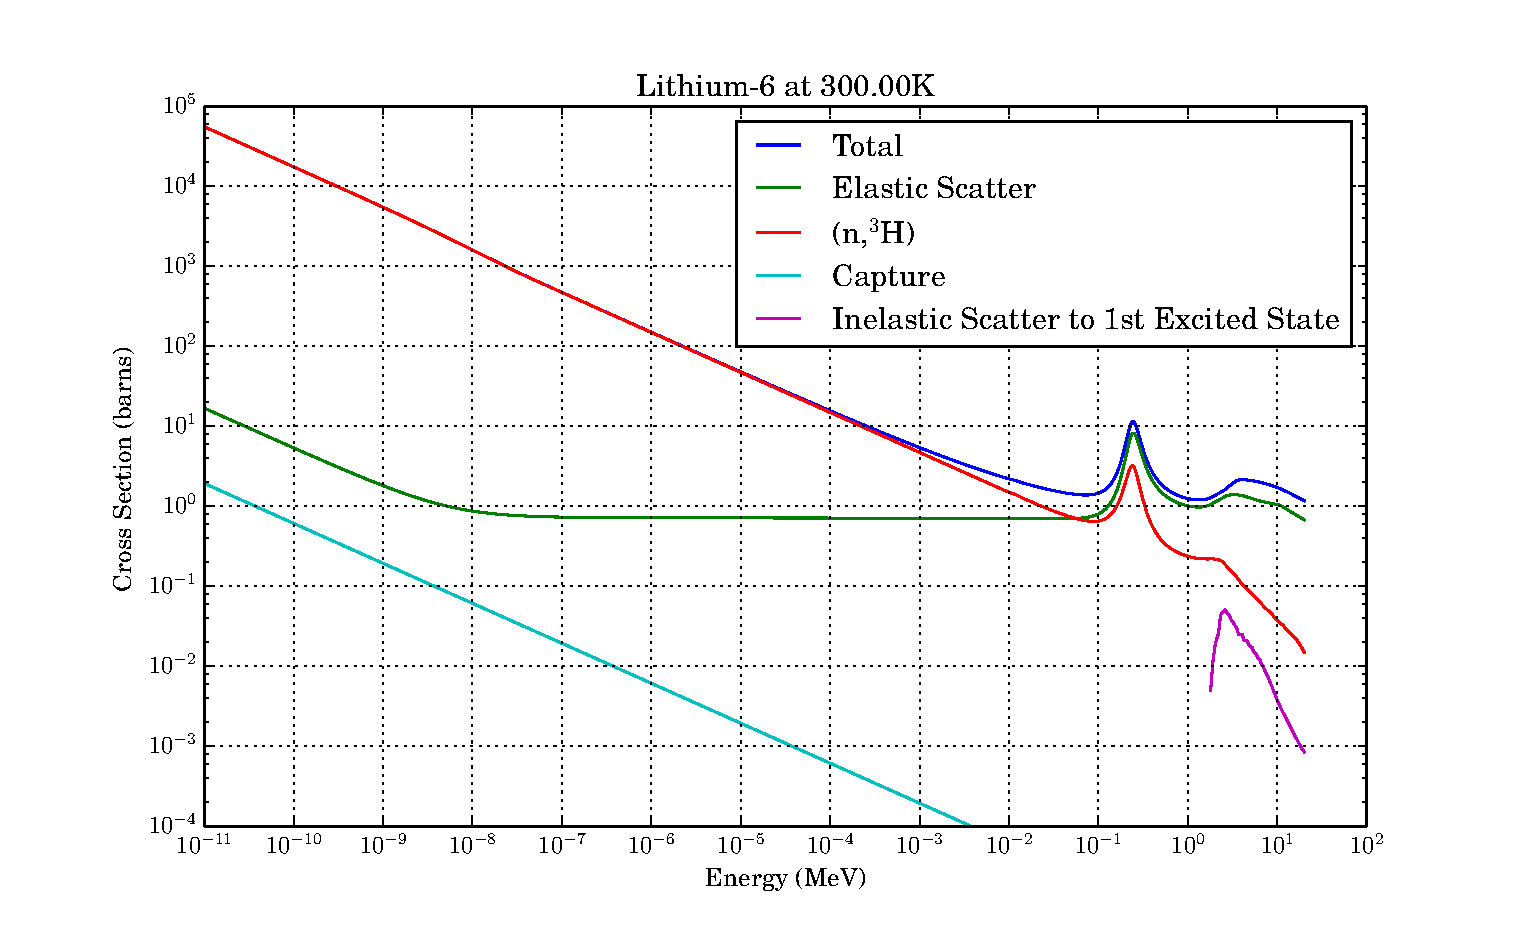
\includegraphics[width=0.8\textwidth]{graphics/xs_li6.eps}
     \caption{The energy dependence of some reactions in $^6$Li.\label{xs_e_dependence_li}}
\end{figure}

\begin{figure}[h!]
  \centering
    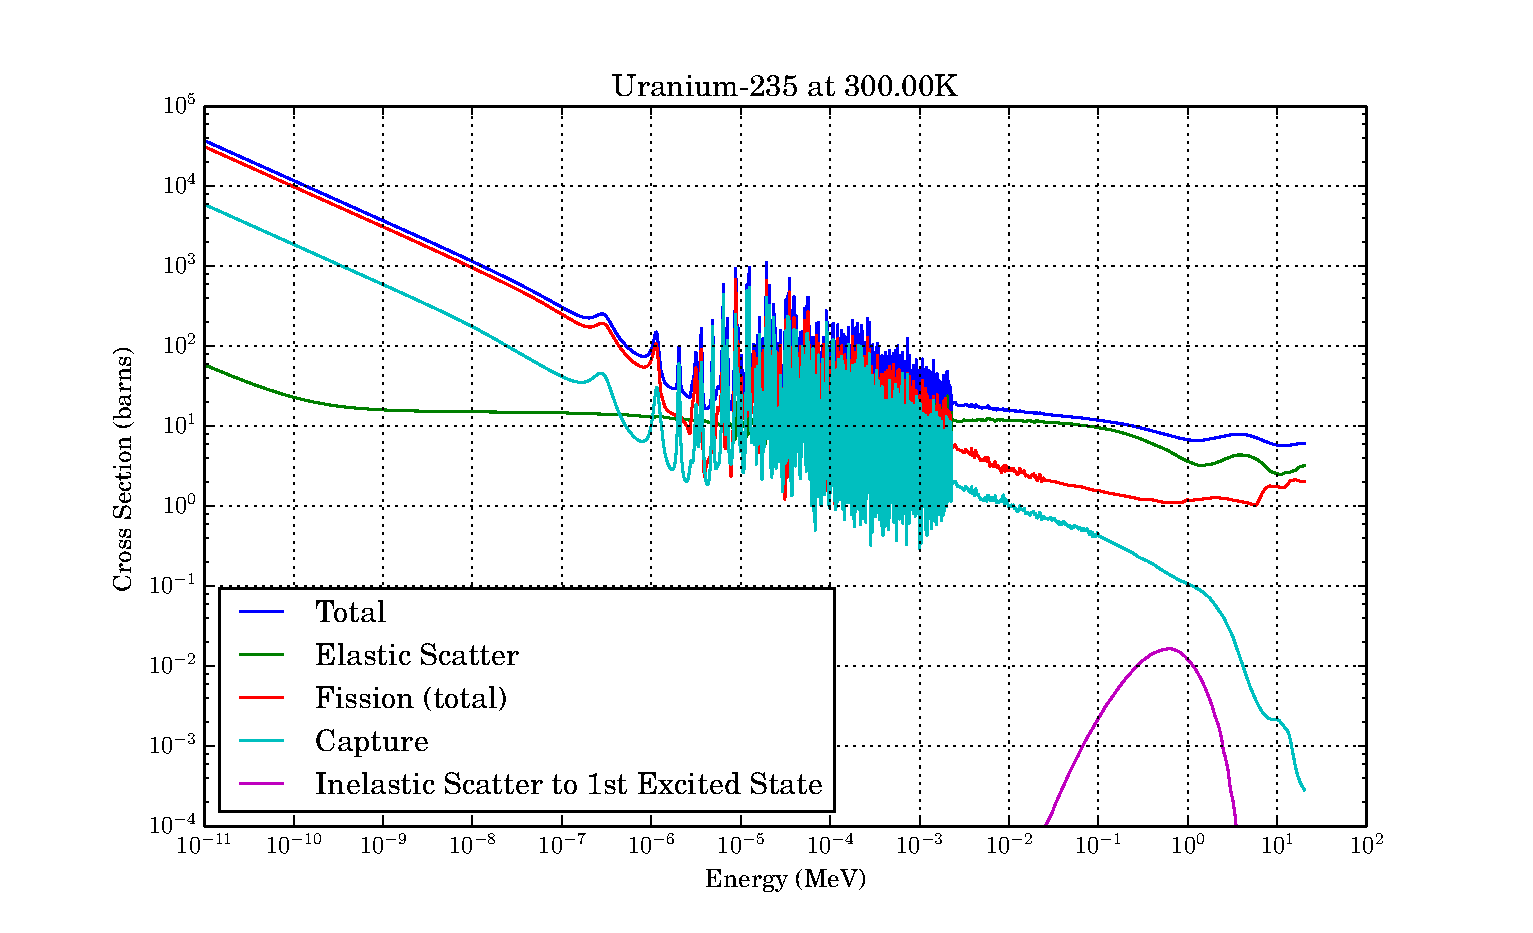
\includegraphics[width=0.8\textwidth]{graphics/xs_u235.eps}
    \caption{The energy dependence of some reactions in $^{235}$U.   \label{xs_e_dependence_u}}
\end{figure}

It is important to note the complexity shown in $^{235}$U in the 0.1 eV to 40 keV range.  This is referred to as the ``resonance region'' and adds much of the complexity in accurately modeling neutron transport.  There are no simple functional representations available for such cross sections, so they must be represented in a point-wise tabular format.  

%It is also important to note that at low energies, cross sections typically exhibit ``1/$v$'' scaling with regard to the incoming neutron energy.  This is due to the particle and the target having more time to interact with each other.  This phenomenon exists at energy levels similar the thermal energy of the target.  Since the neutron has an energy similar to the target, the target no longer appears stationary from the neutron's perspective.  If the neutron is slow enough, the target appears to be moving instead of the neutron, and more targets come into the neutron's sphere of interaction.  This is the qualitative reason for 1/$v$ scaling at low energies.  Because of their identical scaling, the ratios between the reaction types stays constant as velocity is decreased but the overall interaction probability with respect to distance increases \cite{duderstadt}.

\subsection{Elastic Scattering}

Elastic scattering conserves both the momentum and the kinetic energy of the reacting particles and occurs when the neutron does not enter the nucleus, but bounces off of its potential field.  Since there is only a single exiting particle, elastic scattering is a two-body interaction and the kinematics are constrained by conservation of momentum and energy.  The angle between the neutron's incoming and outgoing directions, or scattering angle, $\theta$, is often represented as its cosine, $\mu = \cos \theta$.  The scattering angle is the only unconstrained variable in the elastic scattering interaction, and the exiting neutron energy can be determined if the angle between the incoming and exiting particle is known.  

This problem is greatly simplified if the velocities of the interacting neutron and nucleus are transformed into the center-of-mass (CM) frame, where net momentum is zero. The velocity of the CM is defined in \eqref{vCM} where $m$ and $M$ are the neutron's and the target's respective masses, $v$ and $V$ are their respective velocity vectors, and $A$ is the ratio of the target's mass to the neutron's mass (also know as the ``atomic mass ratio'' or AMR).  The derivation from here follows closely with that in \cite{jaakko}.

\begin{equation}
A = \frac{M}{m}
\label{AWR}
\end{equation}

\begin{equation}
\boldsymbol{\vec{v}_{\mathrm{CM}}} = \frac{ m \boldsymbol{\vec{v}} + M \boldsymbol{\vec{V}} }    {m+M} = \frac{ \boldsymbol{\vec{v}} + A \boldsymbol{\vec{V}} }    {1+A}
\label{vCM}
\end{equation}

The CM velocities of the target and the neutron are then calculated by subtracting the CM velocity out of them, as shown in \eqref{CM}.  The ``$c$'' subscript will denote the CM-frame values from now on, whereas $v_{\mathrm{CM}}$ will denote the velocity of the CM frame relative to the Lab frame.

\begin{equation}
\begin{split}
 \boldsymbol{\vec{v}_{_\mathrm{c}}} &= \boldsymbol{\vec{v}} - \boldsymbol{\vec{v}_{\mathrm{CM}}} \\  
 \boldsymbol{\vec{V}_{\mathrm{c}}} &= \boldsymbol{\vec{V}} - \boldsymbol{\vec{v}_{\mathrm{CM}}}
 \end{split}
\label{CM}
\end{equation}

Once in the CM frame, the equation for conservation of momentum can be written as \eqref{consMomCM}, where the primed values are those after the collision.  Since the net momentum is zero, the neutron and the target must be traveling in exactly opposite directions, as shown in \eqref{rotationCM}.

\begin{equation}
\begin{split}
m \boldsymbol{\vec{v}_{_\mathrm{c}}} + M \boldsymbol{\vec{V}_{_\mathrm{c}}} &= m \boldsymbol{\vec{v}_{_\mathrm{c}}^\prime} + M \boldsymbol{\vec{V}_{_\mathrm{c}}^\prime} = 0\\
    \boldsymbol{\vec{v}_{_\mathrm{c}}} + A  \boldsymbol{\vec{V}_{_\mathrm{c}}} &=     \boldsymbol{\vec{v}_{_\mathrm{c}}^\prime} + A  \boldsymbol{\vec{V}_{_\mathrm{c}}^\prime} = 0
\end{split}
\label{consMomCM}
\end{equation}

\begin{equation}
\begin{split}
\boldsymbol{\vec{v}_{_\mathrm{c}}^\prime} &= - A  \boldsymbol{\vec{V}_{_\mathrm{c}}^\prime} \\
\boldsymbol{\vec{v}_{_\mathrm{c}}} &= -A  \boldsymbol{\vec{V}_{_\mathrm{c}}}
\end{split}
\label{rotationCM}
\end{equation}

The equation for conservation of energy is shown in \eqref{consECM}.  $Q$ is the amount of energy released by the reaction and is zero for elastic scattering.  It is convenient to include in this derivation for use later in inelastic collision kinematics where it is nonzero.

\begin{equation}
\begin{split}
m v_{_\mathrm{c}}^2 + M V_{_\mathrm{c}}^2 &= m v_{_\mathrm{c}}^{\prime2} + M V_{_\mathrm{c}}^{\prime2} + 2Q \\
    v_{_\mathrm{c}}^2 + A  V_{_\mathrm{c}}^2 &=     v_{_\mathrm{c}}^{\prime2} + A  V_{_\mathrm{c}}^{\prime2} + \frac{2Q}{m}
\end{split}
\label{consECM}
\end{equation}

There are now two unknowns (the primed values) and two equations, and the final velocities of the neutron and the target can be determined.  Substituting \eqref{rotationCM} into \eqref{consECM} and solving yields either equation in \eqref{finalvCM}, depending on how the substitution is done.  If $Q$ is zero, as it is in elastic scattering, the initial and final velocities are the same for both the neutron and the target, and the interaction only causes a rotation in the CM frame.

\begin{equation}
\begin{split}
v_{_\mathrm{c}}^{\prime} &=  \sqrt{ v_{_\mathrm{c}}^{2} + \frac{2AQ}{m(A+1)}  }  \\
V_{_\mathrm{c}}^{\prime} &= \sqrt{ V_{_\mathrm{c}}^{2} + \frac{2Q}{mA(A+1)}  } 
\end{split}
\label{finalvCM}
\end{equation}

At first glance, it seems like the interaction has been fully characterized, but \eqref{rotationCM} only relates the initial states of the neutron and the target to one another and the final states of neutron and the target to one another.  The initial state and final state of the neutron still need to be related.  It has been mentioned already that the interaction is only a rotation in the CM frame, so the initial and final state of the neutron's direction can be related by a three-dimensional rotation formula.  

An efficient algorithm is given by \eqref{vector_rot} \cite{openmc}.  In the formula, $\mu=\cos \theta$, and $\hat{{\Omega}}_x$, $\hat{\Omega}_y$, and $\hat{\Omega}_z$ are the cartesian projections of the velocity's unit vector.  It is ``efficient'' in the sense that to rotate a vector, a full 3x3 matrix does not need to be constructed and multiplied by the vector. In other words, matrix-vector operations are not needed and it can be carried out with three scalar operations.

\begin{equation}
\begin{split}
\hat{\Omega}_x^{\prime} &= \mu \hat{\Omega}_x + \frac{\sqrt{1-\mu^2} (\hat{\Omega}_x \hat{\Omega}_z \cos \phi - \hat{\Omega}_y \sin \phi)}{ \sqrt{1-\mu \hat{\Omega}_z^2}} \\
\hat{\Omega}_y^{\prime} &= \mu \hat{\Omega}_y + \frac{\sqrt{1-\mu^2} (\hat{\Omega}_y \hat{\Omega}_z \cos \phi + \hat{\Omega}_x \sin \phi)}{ \sqrt{1-\mu \hat{\Omega}_z^2}} \\
\hat{\Omega}_z^{\prime} &= \mu \hat{\Omega}_z - \sqrt{ (1-\mu^2) (1-\mu \hat{\Omega}_z^2) }  \cos \phi 
\end{split}
\label{vector_rot}
\end{equation}

If the polar and azimuthal rotation angles, $\theta$ and $\phi$, respectively, are determined, the initial neutron velocity vector can be rotated through these angles to its final value.  After the rotation is done, the final velocities are known in the CM frame and they can be transformed back to the Lab frame to give the final velocities there, as shown in \eqref{xformbackCM}.

\begin{equation}
\begin{split}
 \boldsymbol{\vec{v}^{\prime}}  &= \boldsymbol{\vec{v}_{\mathrm{c}}^{\prime}} + \boldsymbol{\vec{v}_{\mathrm{CM}}} \\  
 \boldsymbol{\vec{V}^{\prime}} &= \boldsymbol{\vec{V}_{\mathrm{c}}^{\prime}} + \boldsymbol{\vec{v}_{\mathrm{CM}}}
 \end{split}
\label{xformbackCM}
\end{equation}


\subsection{Inelastic Level Scattering}

\begin{figure}[h!]
  \centering
    \includegraphics[width=0.6\textwidth]{graphics/wiley_levels.pdf}
     \caption[The energy levels of $^{177}$Hf.]{The energy levels of $^{177}$Hf \cite{krane}. \label{Elevels}}
\end{figure}

Inelastic scattering is the other type of scattering a neutron can undergo, but in this case kinetic energy is no longer conserved.  Energy is transferred to or from an internal state of the target nucleus.  This amount of energy, $Q$, is typically defined to be positive for reactions where energy is given to the neutron and the target nucleus, i.e. $Q$ is positive when the sum of the particles' kinetic energies is greater after the reaction than before.  Therefore, $Q$ values for inelastic scattering are negative, since energy is always lost to an internal state of the nucleus.  In neutron-nucleus collisions, the target nucleus can be excited to a higher energy state than its ground state if the colliding neutron has a high enough energy to do so.  If the colliding neutron has enough energy and the collision excites the nucleus, a discrete amount of energy is lost to the reaction.  These excited states typically do not have long half lives, and a gamma ray is emitted when the nucleus relaxes to its ground state.  This type of reaction is called inelastic level scattering because an excited energy \emph{level} becomes occupied by the target nucleus.  

Since this reaction is still a two-body interaction, the kinematics of the reaction are identical to elastic scattering except the $Q$ value is nonzero and negative.  These reactions have a threshold energy below which their cross sections are zero since the neutron would not have enough energy to excite the target nucleus.   Figure \ref{Elevels} shows the energy levels in $^{177}$Hf, which is often used as a thermal neutron absorber due it its large thermal capture cross section, but it  could also be used as a fast neutron moderator because it has many low-lying energy levels and large inelastic scattering cross sections.


\subsection{Inelastic Continuum Scattering}

At energies above the distinct levels there lies a continuum in the nuclear energy states.  This isn't truly a ``continuum'' in a strict sense, but the energy levels become so close together they effectively form a domain where energy can take continuous values.  Unlike the discrete $Q$ values corresponding to a single excited state used in inelastic level scattering, the $Q$ value of the reaction now follows a distribution \cite{krane}.  

\subsection{Fission}

Fission literally means ``the splitting of something into two parts.''  This is exactly what nuclear fission is as well.  Nuclear fission is when a nucleus splits into two smaller nuclei, called \emph{fission fragments}.  When heavy nuclei undergo fission, they release energy and typically emit a few other particles, including neutrons.  That this reaction releases energy is the reason heavy fissile elements, like uranium, can be used as an energy source.  Fission fragments have higher binding energy per nucleon compared to the parent nucleus, and as a result the total mass of the fission products plus initiating neutron is less mass than the parent, meaning there is an energy release.  Figure \ref{binding_e_per_nuc} shows the average binding energy per nucleon for a wide range of nuclides.  Note that the peak of the curve is at iron-56, the most tightly bound nucleus, and that heavier nuclides are lower than it.  Fission splits the parent into two lighter nuclides, and since the fragments are more tightly bound, the excess binding energy from the parent is released.  

The released energy isn't deposited as heat directly, however.  It is released in a range of forms, many of which are converted to heat in the immediate vicinity of the fission event.   Table \ref{fission_dist} shows the fraction of this total energy that is given to each entity \cite{duderstadt}.  Note that a 5\% is given to neutrinos, which is essentially lost because materials have very small neutrino interaction cross sections.  The kinetic energy of the fission fragments has the majority of the energy, and since they are heavy and charged, their energy is deposited as heat very near to the fission site.  Other particles carry some of the fission energy further away from the fission site, but their energy is still almost all converted to heat.  
  
\begin{figure}[h!]
  \centering
    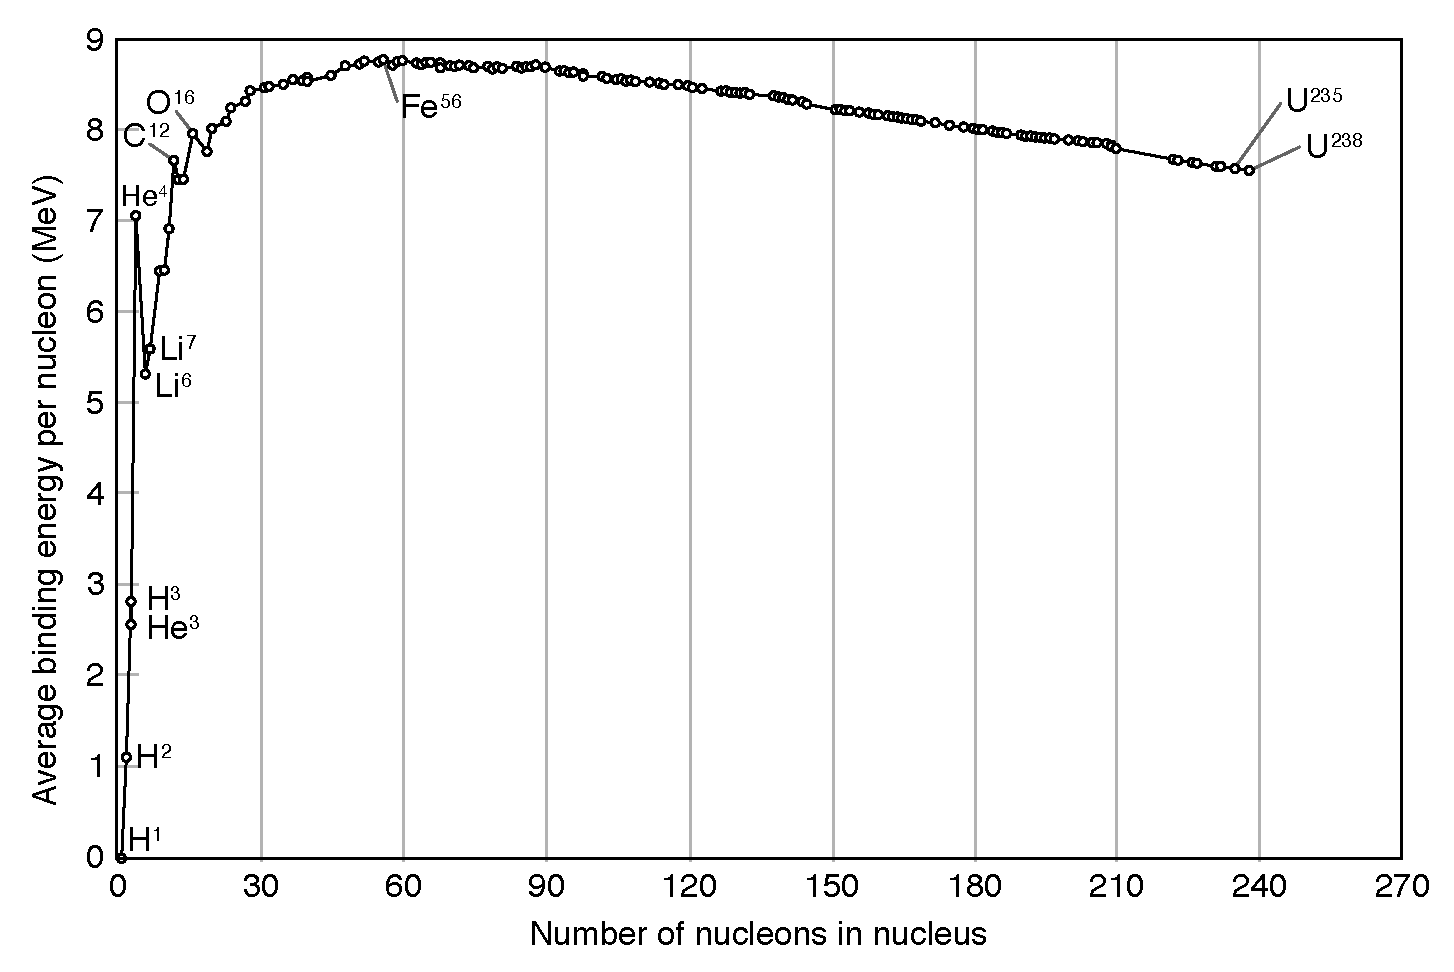
\includegraphics[width=0.8\textwidth]{graphics/binding_energy.pdf}
     \caption[Average binding energy per nucleon.]{Average binding energy per nucleon \cite{wikimedia_binding}.\label{binding_e_per_nuc}}
\end{figure}

\begin{table}[h]
\centering
\caption[Average distribution of fission energy.]{Average distribution of fission energy \cite{duderstadt}.\label{fission_dist}}
\begin{tabular}{| l | c | r | r |}
\hline
Particle & Energy (\%) & Range & Time \\
\hline
Fission fragment kinetic energy & 80 & $<$0.1cm & prompt \\
\hline
Prompt neutrons & 3 & 10-100cm & prompt \\
\hline
Photons & 4 & 100cm & prompt \\
\hline
Fission product $\beta$ decay & 4 & short & delayed \\
\hline
Neutrinos &  5 & extremely long & delayed \\
\hline
Nonfission reactions from n capture & 4 & 100cm & delayed \\
\hline
\end{tabular}
\end{table}

Fission is technically considered an absorption reaction since the fission-inducing neutron enters the nucleus and creates a compound nucleus.  Even though the neutron is absorbed, on average more than two new neutrons are released by each fission, enabling a fission chain reaction.  An important parameter of the fission chain reaction is $\nu_\mathrm{T}$, the average total number of neutrons emitted per fission.  This number is called ``total'' since includes prompt neutrons, which appear immediately after fission, and delayed neutrons, which appear later.  Delayed neutrons are mainly produced from fission product decay, but a small fraction also comes from photon-induced emission.  These neutrons are not ``prompt'' in that they are not emitted immediately from the fission itself.  The processes that create these ``delayed'' neutrons (decay and nuclear relaxation) take time to occur and these neutrons can therefore appear anywhere between 0.6 to 80 seconds after a fission event \cite{duderstadt}. 

The kinetics of a nuclear chain reaction depends heavily on the mean neutron lifetime, as was shown by the point kinetics equation in \ref{sec:analysis}.  If only prompt neutrons are considered, the mean neutron lifetime is approximately $10^{-4}$ seconds in light water (thermal spectrum) reactors fueled by $^{235}$U \cite{duderstadt}.  Having a reactor that is critical solely on prompt neutrons means that it's power can change on the order of the prompt neutron lifetime.  At this speed, it would be difficult for control systems to respond in time to suppress any power excursions before damage occurred.  This is where delayed neutrons come into play.  If a reactor is not critical with prompt neutrons, but is critical with the incorporation of the delayed neutrons, the long appearance time of delayed neutrons shifts the mean neutron lifetime to larger values; typically to around 0.1 seconds for light water reactors \cite{duderstadt}.  The reactor is much easier to control with this much slower mean neutron lifetime.

% for context, you should probably talk about prompt neutron lifetime of at least U235 fissions...
% wait, we usually bundle the generations together to get one effective neutron lifetime. this paragraph doesn't make sense b/c you start out talking about how we need delayed neutrons to slow down the generation time, and end with two different times.
% I have changed these paragraphs to be more clear, I hope.

\begin{figure}[h!]
  \centering
    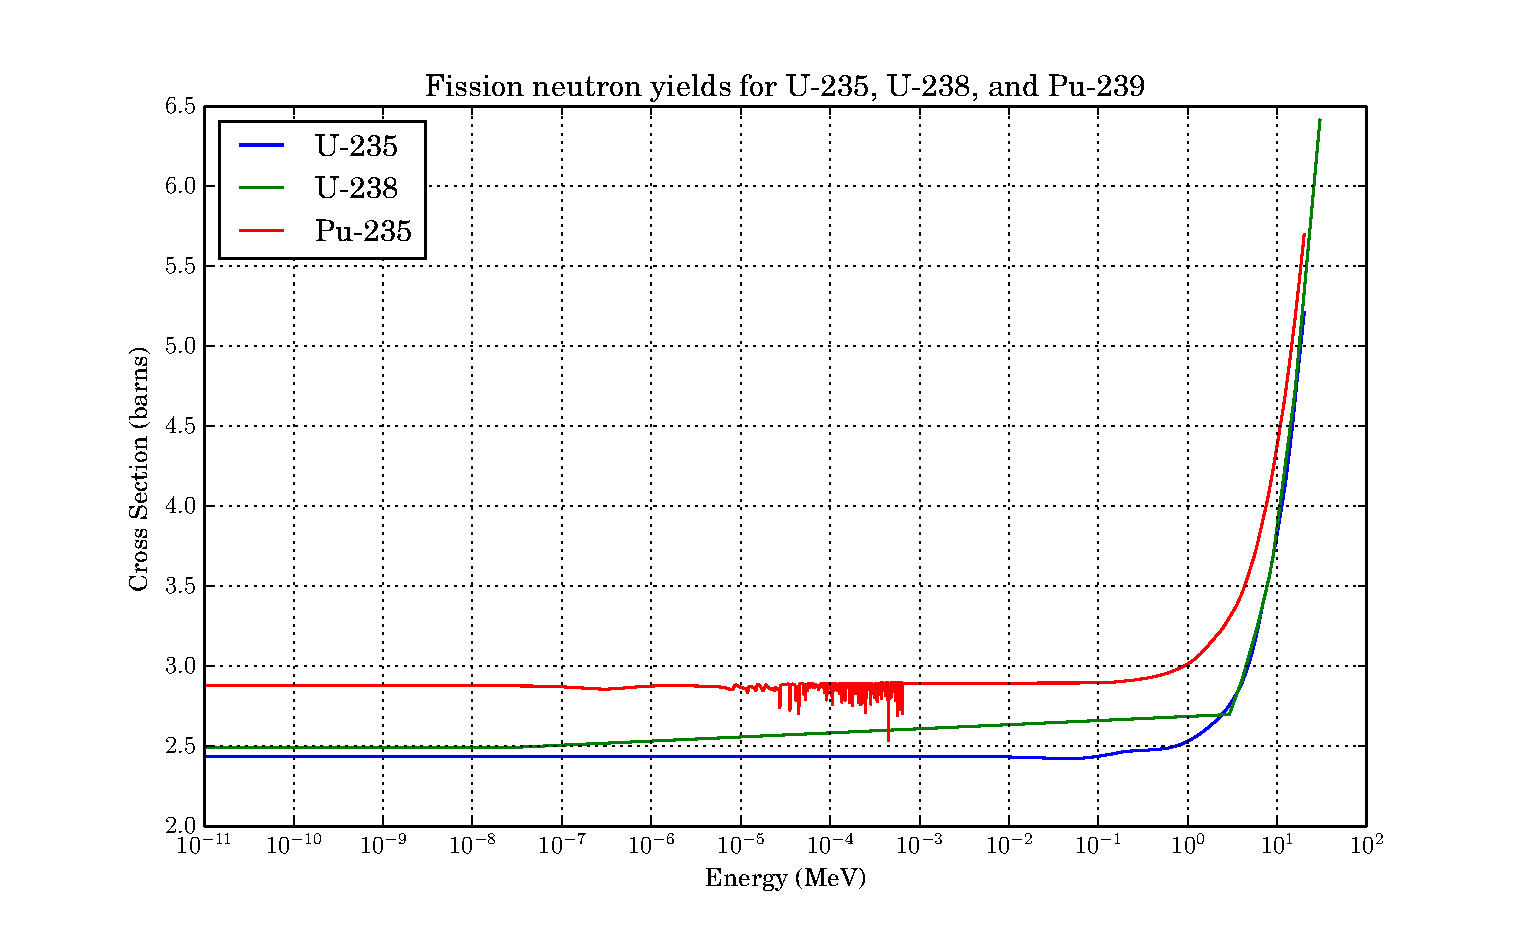
\includegraphics[width=0.8\textwidth]{graphics/nu_compare.eps}
     \caption{The average total number of neutrons per fission, $\nu_\mathrm{T}$, for $^{235}$U, $^{238}$U, and $^{239}$Pu. \label{nu_compare}}
\end{figure}

\begin{figure}[h!]
  \centering
    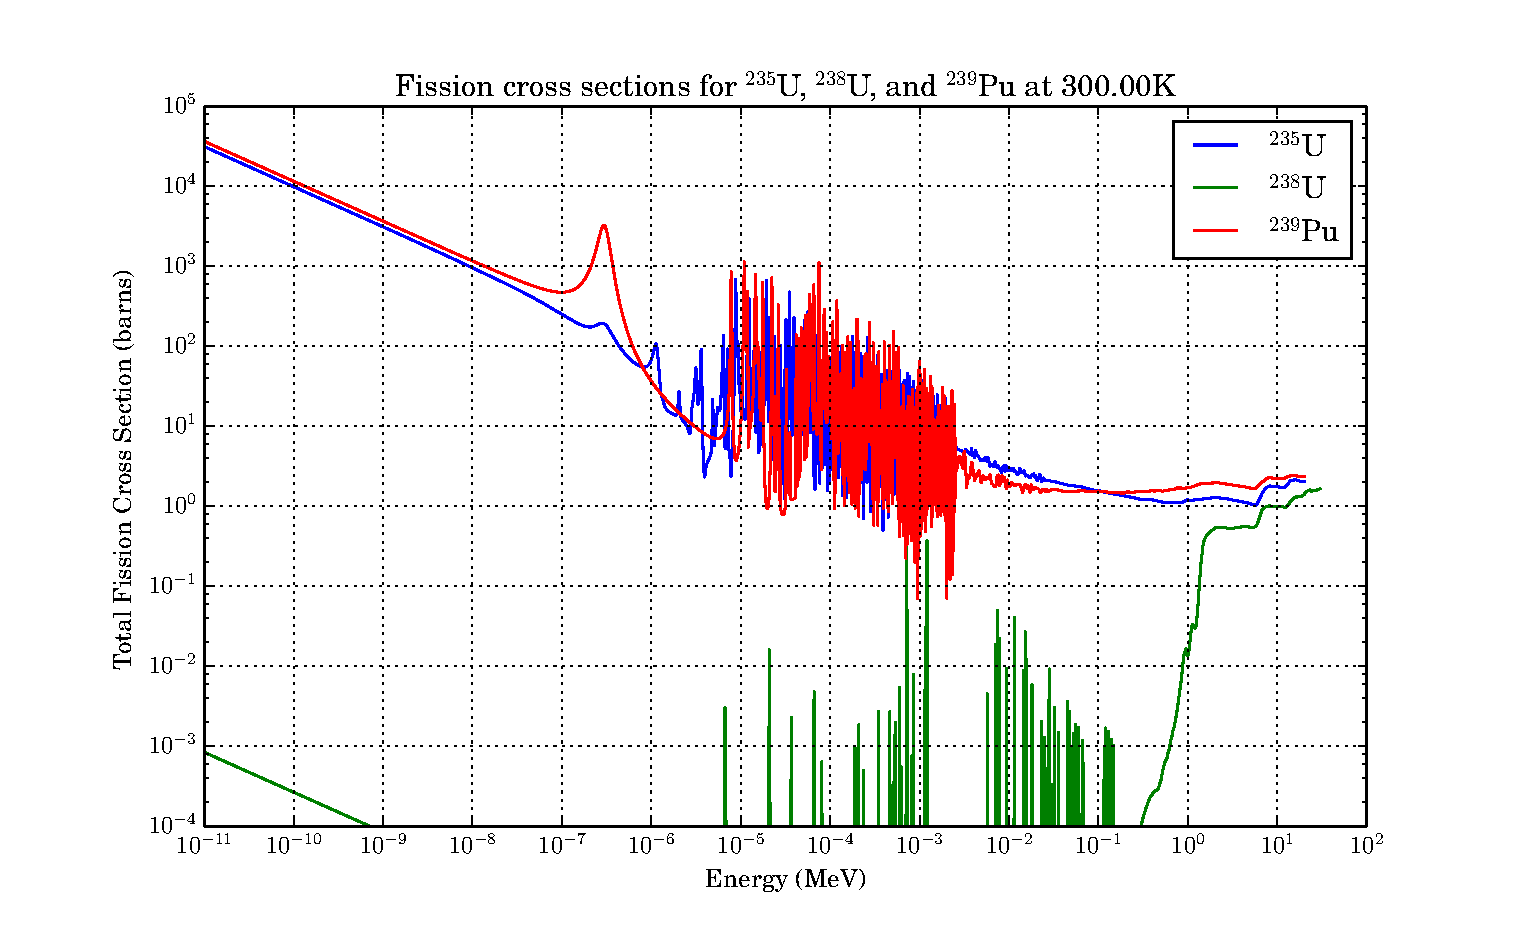
\includegraphics[width=0.8\textwidth]{graphics/xs_fissile.eps}
     \caption{Fission cross sections for $^{235}$U, $^{238}$U, and  $^{239}$Pu. \label{xs_fission_only}}
\end{figure}

Figure \ref{nu_compare} shows the energy dependence of the average total number of neutrons per fission, $\nu_\mathrm{T}$, for several fissionable isotopes.  $\nu_\mathrm{T}$ is shown at a single target material temperature since it has very weak temperature dependence for most incoming neutron energies.   For all three isotopes shown, $\nu_\mathrm{T}$ is nearly constant from low energies up to energies in the MeV range, where it increases sharply due to the energy the incident neutron provides being sufficient to eject additional bound neutrons.  

% Okay, I got to here and had thought \nu up above was total. what does \nu include then? I'm confused by your previous discussion now. I have relabeled it so I am always talking about nu_T
% In this discussion you should indicate which \nu_T you're talking about or talk about them collectively (the figure has 3 values)
%  I am speaking about nu_T in general.  I never once mention a specific value for it, I only am discussing what it means and the figure is for illustration

Figure \ref{xs_fission_only} shows the total fission cross sections for two fissile isotopes, $^{235}$U and $^{239}$Pu, and one fertile isotope, $^{238}$U.  The figure shows that  $^{238}$U has a fission cross section, but it isn't significant until above 1 MeV.  For $^{238}$U, fission is practically a threshold reaction.  Simply absorbing a neutron does not provide enough energy to split the nucleus.  Additional energy is required, which can be provided in the form of an incident neutron's kinetic energy.  $^{238}$U isn't fissile, but it can be a significant contributor of fission reactions in reactors where the neutron population is \emph{fast}, i.e.\ mainly high-energy.  As mentioned before, $^{238}$U is considered fertile because it is converted to the fissile isotope $^{239}$Pu \cite{duderstadt}.  
  
WARP uses $\nu_\mathrm{T}$ and fission neutron energy spectra that incorporate delayed neutron energies since is more physically accurate and produces the overall effective multiplication factor.  

\subsection{Capture Reactions}

Unlike scattering reactions, where the energy and direction of the neutron is changed but continues to transport, \emph{disappearance} reactions remove a free neutron.  Typically this \emph{capture} of a neutron leaves the daughter nucleus in an excited state, which them relaxes to ground state by emitting a gamma ray \cite{krane}.


\subsection{Other Secondary-Producing Absorption Reactions}

This category encompasses all the other reactions neutrons undergo.  There are two types: reactions that produce secondary neutrons in some amount and reactions that do not.  Those that do not may still produce other particles, like alpha particles, tritons, protons, et cetera.  Since these do not produce secondary neutrons, however, they are basically equivalent to capture reactions from a neutron transport standpoint.  Even though they aren't strictly capture reactions, they can contribute significantly to an isotope's absorption of neutrons.  Figure \ref{xs_e_dependence_li} shows that the (n,$\alpha$) in $^{10}$B is by far the main component of the total cross section, making $^{10}$B a very strong absorber of low energy neutrons.  $^10$B is widely used in safety and control systems in thermal-spectrum reactors.

Of the reactions that produce secondary neutrons, the (n,2n) reaction is most significant because it has the lowest threshold energy.  At higher incident neutron energies, (n,3n) and even (n,4n) can become possible.  Other particle combinations are possible as well, such as (n,n$\alpha$), and these reactions act like an inelastic scatter interaction where the relationship between scattering angle and energy no longer applies due to there being three bodies to distribute energy to instead of only two.

\subsection{Bound Nuclei and Unresolved Resonances}

Treating matter as a collection of free nuclei is a good approximation most of the time since the neutron energies are much larger then the thermal energies of the nuclei, and the recoil energies imparted on the targets is typically much larger than any cohesive forces between them \cite{jaakko}.  This assumption is not valid for many important moderator materials like water and graphite.  In these materials, the atoms are bonded to each other and provides another degree of freedom for energy transfer in scattering.  Since the bounds are of the same energy as a low energy neutron, when the neutron scatters off bound nuclei, a significant amount of energy can be lost to breaking these bonds.  This changes the scattering kinematics significantly and the reactions rates can be significantly effected from this change \cite{jaakko}.  The kinematics of thermal scattering are handles via the S($\alpha$,$\beta$) coupled energy-angle representation, which replaces the free gas treatment discussed in the following section \cite{mcnp}.  WARP does not included the S($\alpha$,$\beta$) treatment currently.  Adding it will be a point of future development.

There is also a special treatment for sampling reaction types in the unresolved resonance region that is not implemented in WARP.  The unresolved resonance region is the energy range above the resolved resonance region (e.g. 2.25 - 25 keV for $^{235}$U) where the resonances are so closely spaced together that the cross section appears to be smoothly-varying \cite{mcnp}.  Treating the cross sections as smooth in this region does not account for resonance self-shielding effects, and can produce inaccurate results in systems where the flux is large in this region.  Resonance self shielding is where the flux near a resonance becomes depressed due to strong absorption in the resonance, and this flux depression ``shields'' the nuclei from neutrons at this energy \cite{duderstadt}.  Probability tables are included in ENDF data to account for these resonances, but these tables are not loaded by WARP.  Adding the unresolved resonance treatment will be another point of future development for WARP.

%%%%%%%%%%%%%%%%%%%%%%%%%%%%%%
\section{Temperature Effects}
\label{sec:temp}

Thus far there has only been mention of the target nuclide's velocity by how it manifests itself in the 1/$v$ behavior of cross sections at low energy.  It is a good assumption that the thermal motion of the target nuclide is negligible when neutrons are at MeV-range energies.  However, when neutrons scatter and lose energy they can come near the thermal energy of the material, which is on the order of .01 eV.  When this happens, the target nuclide no longer appears stationary, and assuming that it has zero velocity in scattering calculations is inaccurate as discussed above. 

MCNP sets the threshold above which the target nuclide can be assumed stationary at 400 kT, which corresponds to about 10 eV for materials at room temperature \cite{mcnp}.  Below this threshold, it is important to model thermal effects.  If this wasn't done, a neutron could keep scattering off of zero-energy targets and its energy could approach zero, which is not physical.  Neutrons can only scatter down to a state where they are in thermal equilibrium with the material they are traveling through.  This creates a ``thermal peak'' at low energies where neutrons collect, especially in materials where the absorption-to-scattering cross section ratio is small and neutrons scatter many times before they are absorbed.

\subsection{Doppler Effect}

\begin{figure}[h!]
  \centering
    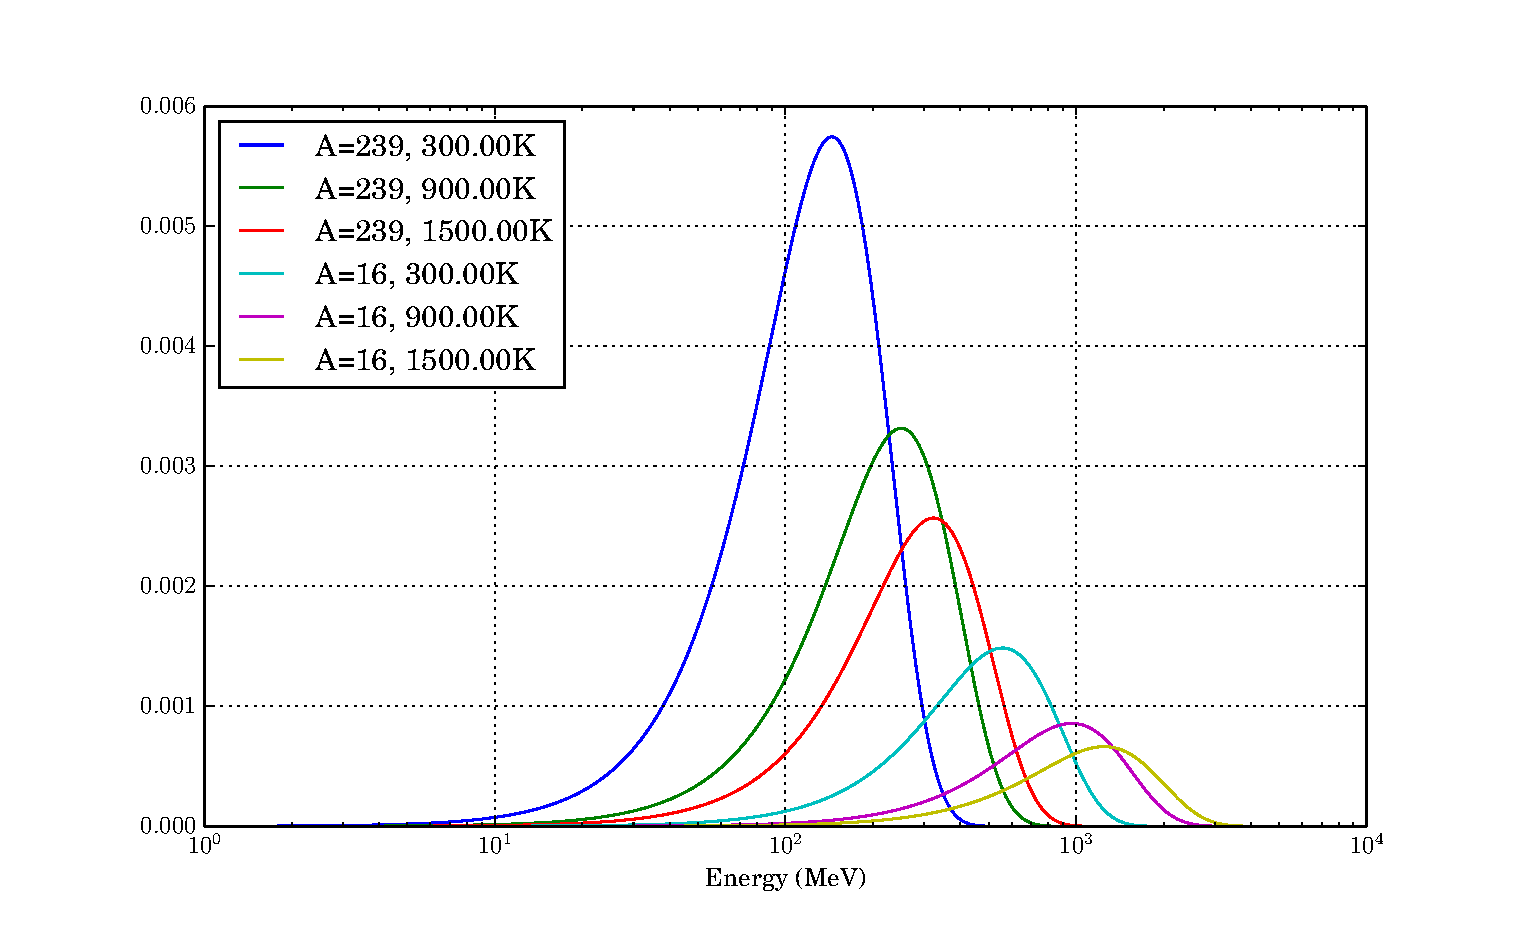
\includegraphics[width=0.8\textwidth]{graphics/MB_dist.eps}
     \caption{Maxwell-Boltzmann distribution for the speed of heavy and light nuclides at different temperatures.   \label{MB_dist}}
\end{figure}

The other effect that thermal motion has is the \emph{Doppler effect}.  The nuclei in a material are assumed to be in thermal equilibrium, and the velocities of the nuclei follow a Maxwell-Boltzmann distribution with a mean value corresponding to the material's temperature.  Cross section data is adjusted to preserved true reaction rates even though target nucleus is assumed to be at rest.  This adjustment basically involves convolving the cross sections with the thermal distribution of the target velocities.  When temperature rises, the thermal velocity distribution becomes wider, and this manifests itself in the cross sections by broadening resonance.  The effect is also known as \emph{Doppler broadening}, named after the Doppler effect, which describes how spectral lines are shifted based on the relative velocities of the emitter and the receiver.  Figure \ref{MB_dist} shows the Maxwell-Boltzmann distributions at various temperatures for a heavy nucleus and for a light nucleus.  This is the distribution of speeds particles in a ``gas'' have if they only interact by scattering off of one another.  Most solids can be modeled as a dense gas when there are no strong anisotropies in their structure, which is why modeling the target velocities in this way is called the ``free gas model.''  Note that the broadening effect is much more pronounced for light nuclei \cite{duderstadt}.  % you sort of describe this above as well (I think) in case you want to refer to that.  Hmmmm, I don't think I do.  I may have mentioned it, but no details, so I'd like to keep this

The widening of resonances affects reactors in significant ways.  The most notable is that absorption probability in resonances increases in the resonance region as neutrons scatter down to thermal energies.  Since the number of neutrons lost to capture increases, Doppler broadening reduces the overall multiplication factor.  It is important for reactor safety that this occurs since it produces a negative reactivity feedback for fuel temperature increase and helps prevent power excursions and meltdowns.  If the multiplication factor is above unity, the power starts to rise.  In the short term, the fuel temperature will rise more rapidly than any coolant mechanism can respond, so a increase in power corresponds directly to an increase in fuel temperature.
% I don't think you need the assumption because the temperature in the fuel will rise more rapidly than any coolant mechanism can respond, which is why the doppler effect always applies at least in an instantaneous sense.  DONE.
  When the temperature goes up, the increased captures causes the fission rate and thus temperature to decrease, stopping the power from increasing \cite{duderstadt}. There are many different types of reactivity feedback phenomena, but the fuel temperature feedback is generally negative because of Doppler broadening.  
  
Capture increases most in fission products since they often have strong absorption resonances and are lighter than fuel nuclides.  Very light nuclides typically do not have absorption resonances, so Doppler broadening has littler effect on their absorption rates.
% You don't ever tell us what fuel is made of, so we don't know what proportion is light. Actually, you don't ever tell us about what fission products are either (though without that this part still makes sense so long as you explain fuel).  added description in the beginning.
  This is why temperature feedback is least effective in fresh fuel where there are few fission products.  Figure \ref{xs_eu_broaden} shows the effect in  $^{155}$Eu, a fission product with a high capture cross section.

\begin{figure}[h!]
  \centering
    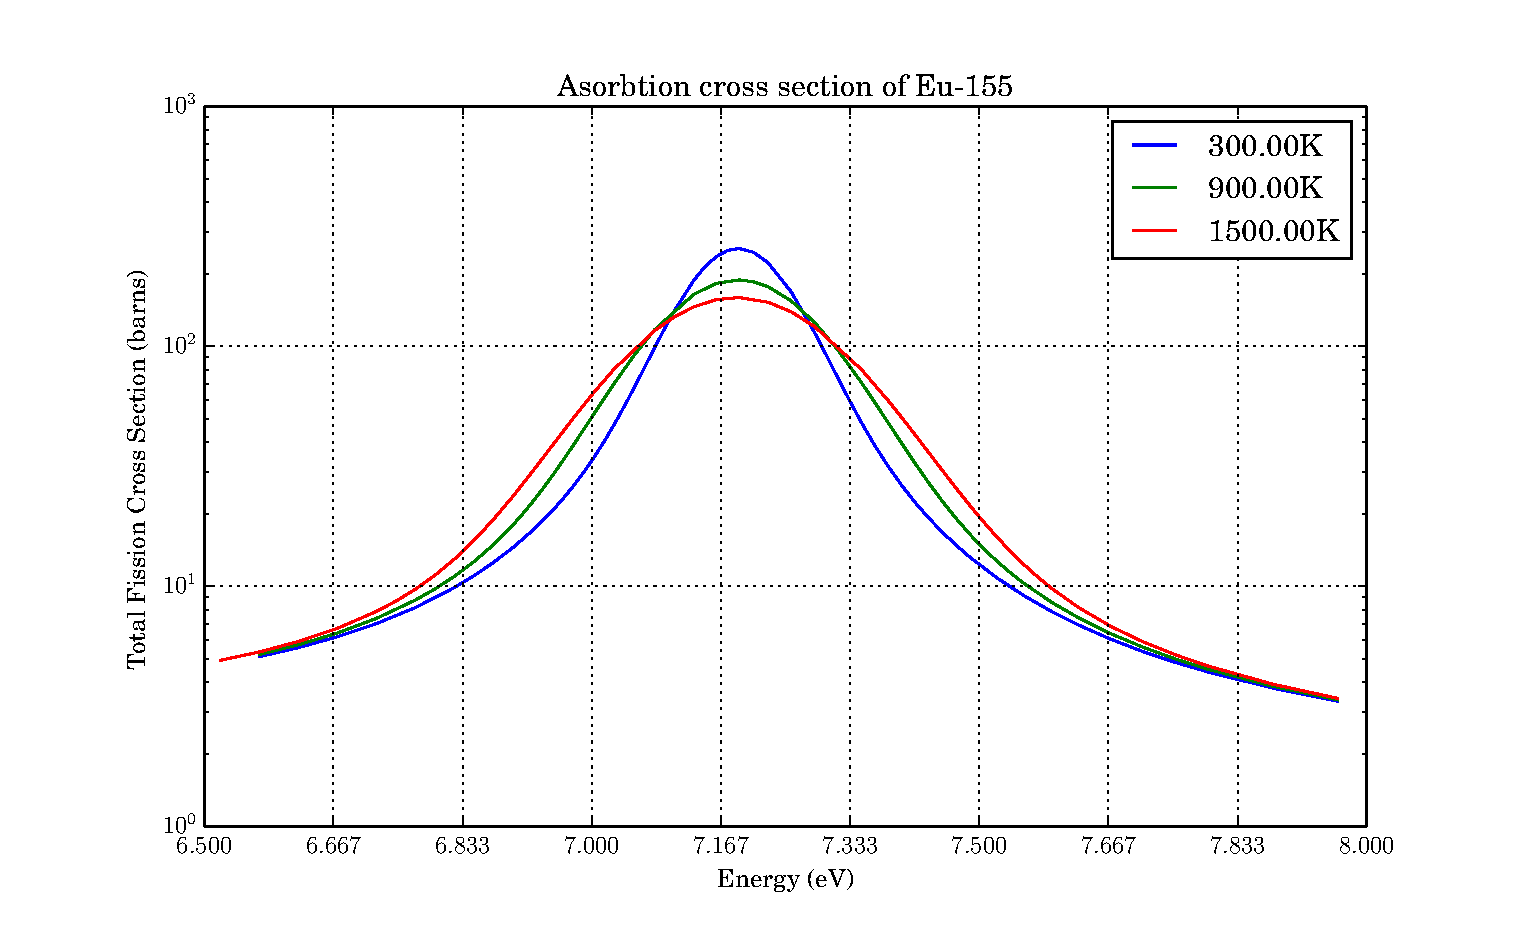
\includegraphics[width=0.8\textwidth]{graphics/xs_eu_broaden.eps}
     \caption{Doppler broadening of the 1 eV fission resonance in  $^{155}$Eu.  \label{xs_eu_broaden}}
\end{figure}

%At 0 K, resonances are very sharp and can be treated as delta functions \cite{duderstadt}. you need to connect this idea more clearly to the rest of the paragraph.
%Reaction rates depend on the relative velocity of the neutron and the target nuclide, and since the target nuclides have a spectrum of energies, the relative velocity does as well.  
The way cross sections are processed assumes that the target nucleus will be treated as being at rest.  This is not physically true, since the nuclei have velocities that follow a thermal distribution.  This distribution of target velocities gives relative velocity of a neutron and the nuclei the same distribution.  Since the cross section actually depends on the relative velocity, the total reaction rate of a neutron at a specific energy is the sum of the reaction rates across all the relative velocities present due to thermal motion of the targets.  The accurate total reaction rate can be preserved even if the target is assumed at rest if the thermal motion effect has already been incorporated into the cross section.  This temperature processed cross section is a called a \emph{thermally averaged} cross section, $\bar{\sigma}$. It can be used in simulations assuming a target at rest, and the simulation will produce the same results as one that explicitly models the target thermal motion.  The effects of thermal averaging are especially significant at resonances since slight movements in velocity can produce very large differences in cross section.  The overall effect is that sharp resonances are \emph{effectively} broadened since they start to contribute to reaction rates, and therefore thermally averaged cross sections, once the thermal distribution of relative velocities starts overlap them.  
% This whole paragraph is kinda confusing. I tried to make it a little more clear, but I'm not sure I was successful.  I hope its better now :/
 
The expression for thermally-averaged cross sections is shown in \eqref{broaden} \cite{openmc}, where $v_n$ and $\boldsymbol{v_n}$ are the speed and velocity of the neutron, respectively, $\boldsymbol{v_t}$ is the velocity of the target, $v_\mathrm{rel} = || \boldsymbol{v_n} -\boldsymbol{v_t}||$ is the velocity of the neutron relative to the target, and $M(v_t)$ is the thermal distribution of target speeds.  

\begin{equation}
\bar{\sigma} = \frac{1}{v_n} \int v_\mathrm{rel} \sigma(v_\mathrm{rel}) M(v_t) dv_t
\label{broaden}
\end{equation}

The fact that cross sections have been adjusted for a material temperature will be significant in Section \ref{sec:MC} when the target-at-rest assumption breaks down and it becomes necessary to preserve the correct reaction rates while still using the temperature-processed cross sections.

%%%%%%%%%%%%%%%%%%%%%%%%%%%%%%
\section{Nuclear Data}

Cross section data compiled by the United States is distributed by the Department of Energy in \emph{ENDF} files.  ENDF stands for ``evaluated nuclear data file,'' and can contain data for nuclear decay, photons, atomic relaxation, fission yields, thermal neutron scattering, and charged particle reactions as well as neutron reactions.  The data files are called ``evaluated'' because a group of experts decides, or evaluates, what data is included in them.  The data includes theoretical calculations of cross sections based on well developed models as well as experimental data.  They also decide how to represent regimes that haven't been measured yet by comparing simulation results to experiments.   The first data released was ENDF/B-I in 1968 and the latest set is ENDF/B-VII, which was released in 2006.  

The data is written in a standard format that dates back to when the data was stored on magnetic tapes, and data entries are sometimes referred to as ``tapes'' to this day.  The format is rather archaic and contains a lot of redundant information about record locations, which was useful when the tape head had to physically move between points in the tape \cite{endfnums}.  

\begin{figure}[h!]
  \centering
    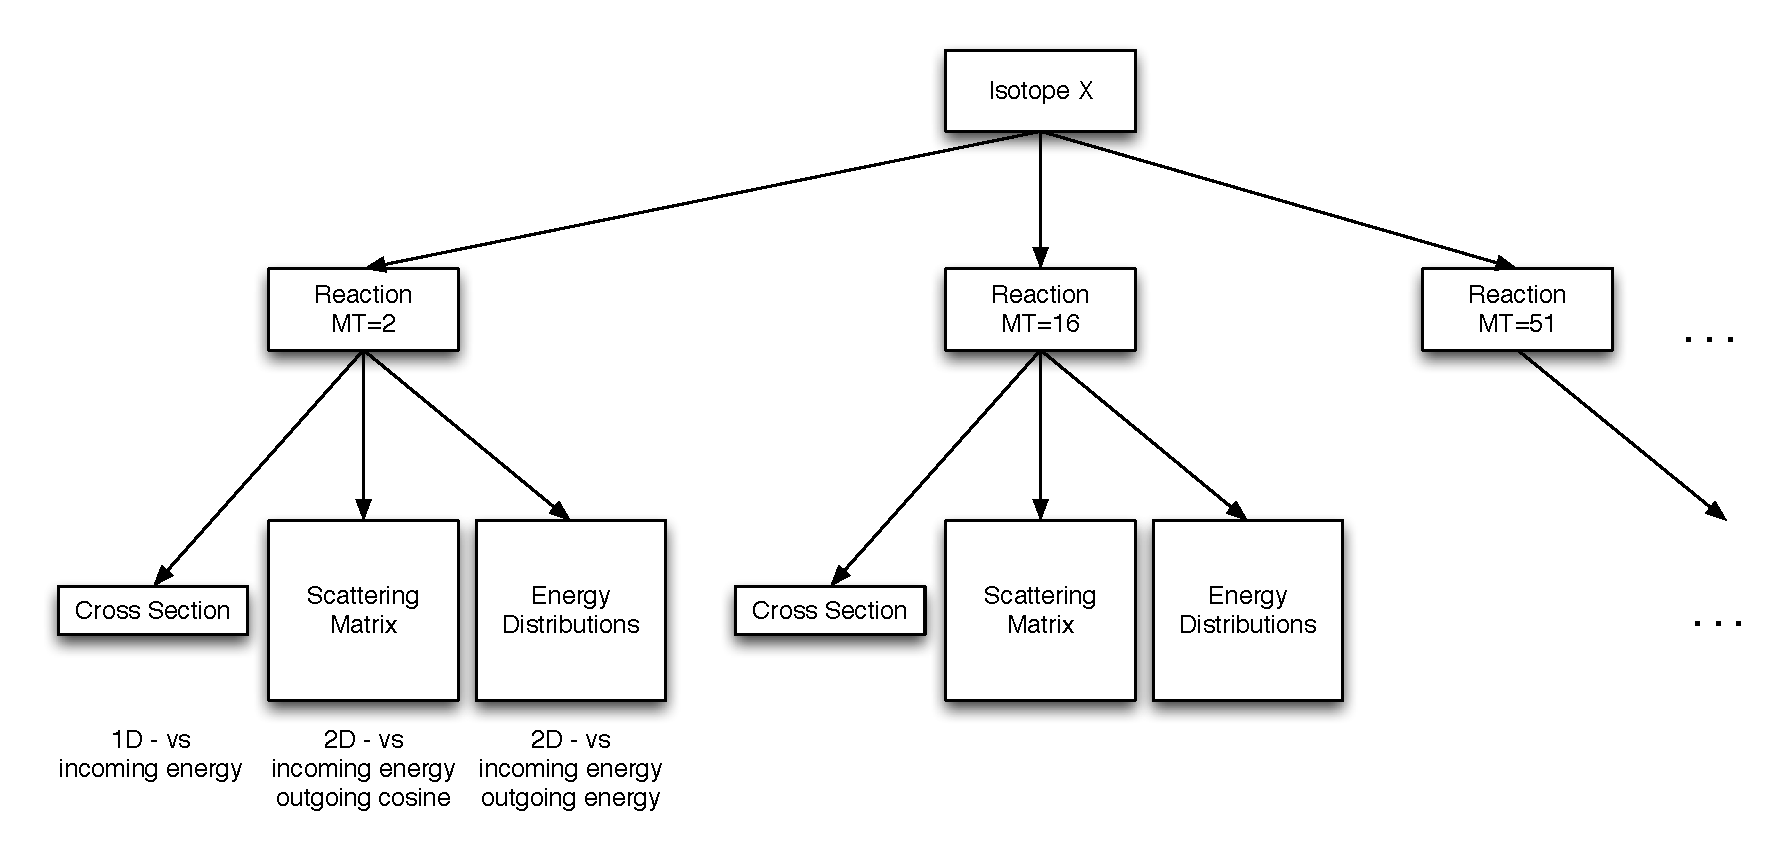
\includegraphics[width=0.8\textwidth]{graphics/data_levels.eps}
     \caption{Hierarchy in ACE formatted neutron data libraries.  \label{data_levels}}
\end{figure}

Many Monte Carlo codes read ACE-formatted data rather than the original ENDF file.  ENDF files contain a lot of data so the dataset preserves the original evaluation, but most transport codes need the data in tabular format.  This is why transport codes normally use ACE-formatted data files. \cite{jaakko}  ACE stands for ``a compact ENDF'' and strips out a lot of the extra information unnecessary for neutron transport.  ENDF tapes contain information that is valuable for charged particles and photons as well as neutrons, and this information is discarded for neutron transport. As Figure \ref{data_levels} shows, ACE files not only contain cross sections, but also angle and energy distributions used in scattering and fission.  ENDF assigns a number to each type of reaction called the \emph{MT} number.  Table \ref{MT_numbers} in Appendix B, taken from a LANL website, shows what these MT numbers mean \cite{endfnums}.  

It can clearly be seen that there are many reactions a neutron can undergo, most of which have very strong energy dependence.  Most of the complexity in modeling nuclear reactors comes from the fact that the data needed to model neutrons is very complicated.  Data may be the most important part of the simulation; it is what ties the calculations to reality.  

ACE data files typically come pre-processed at different temperatures.  This processing can done by a code called NJOY \cite{jaakko}, which Doppler broadens all the resonances in the cross sections and adjusts and unresolved resonance tables accordingly.  It can also thin the energy grid if requested by the user, though this reduces the accuracy of the cross sections \cite{jaakko}.  Thinning the energy grid is a computationally intensive task, and NJOY is not parallelized.  Most production codes come with their own pre-processed datasets at several temperature intervals in order to save the user the time and effort needed to process data from ENDF files.


%%%%%%%%%%%%%%%%%%%%%%%%%%%%%%
\section{Neutron Transport}

Now that the events that can happen to neutrons have been outlined, we will move to describing the neutron population itself.  Since the neutron population in reactor cores is large, on the order of $10^{8}/\mathrm{cm}^3$ \cite{duderstadt}, the neutrons themselves have very small radii, about $1.75\times10^{-17}$ cm \cite{krane}, and only the average behavior matters, their discrete distribution can be well-approximated by a continuous distribution function.  We will eventually derive the \emph{neutron transport equation}, which is a linearized version of the Boltzmann transport equation.  It is linear since it is assumed that neutrons do not interact with each other.  This is usually a good assumption in normal matter since the neutron density present in reactors is many orders of magnitude smaller than the material density and neutrons are much more likely to interact with the nuclei than each other \cite{duderstadt}.  
`
Other than eliminating neutron self-interaction, there are several assumptions that go into the equation that will hold true for the rest of the derivations.  The first is that neutrons are assumed to be points in space, so even at very high densities they still will not interact with each other and later, when we start to discretize space, neutrons cannot be in more than one unique volume by overlapping.  The next assumption is that any relativistic effects are negligible.  The energies of importance in reactor physics are below 10 MeV, far below the neutron rest mass, and any changes in neutron mass will be below 1\%.  Since neutrons are neutral, they are assumed to move in straight lines between collisions.  Materials are also assumed to be in thermal equilibrium and to have isotropic properties \cite{duderstadt}.  Some common reactor materials like graphite and water do not have isotropic properties when it comes to scattering, however.  As will be explained later, this can be corrected for by adjusting the scattering kernel.

\subsection{Neutron Balance Equation}

\begin{figure}[h!] 
  \centering
    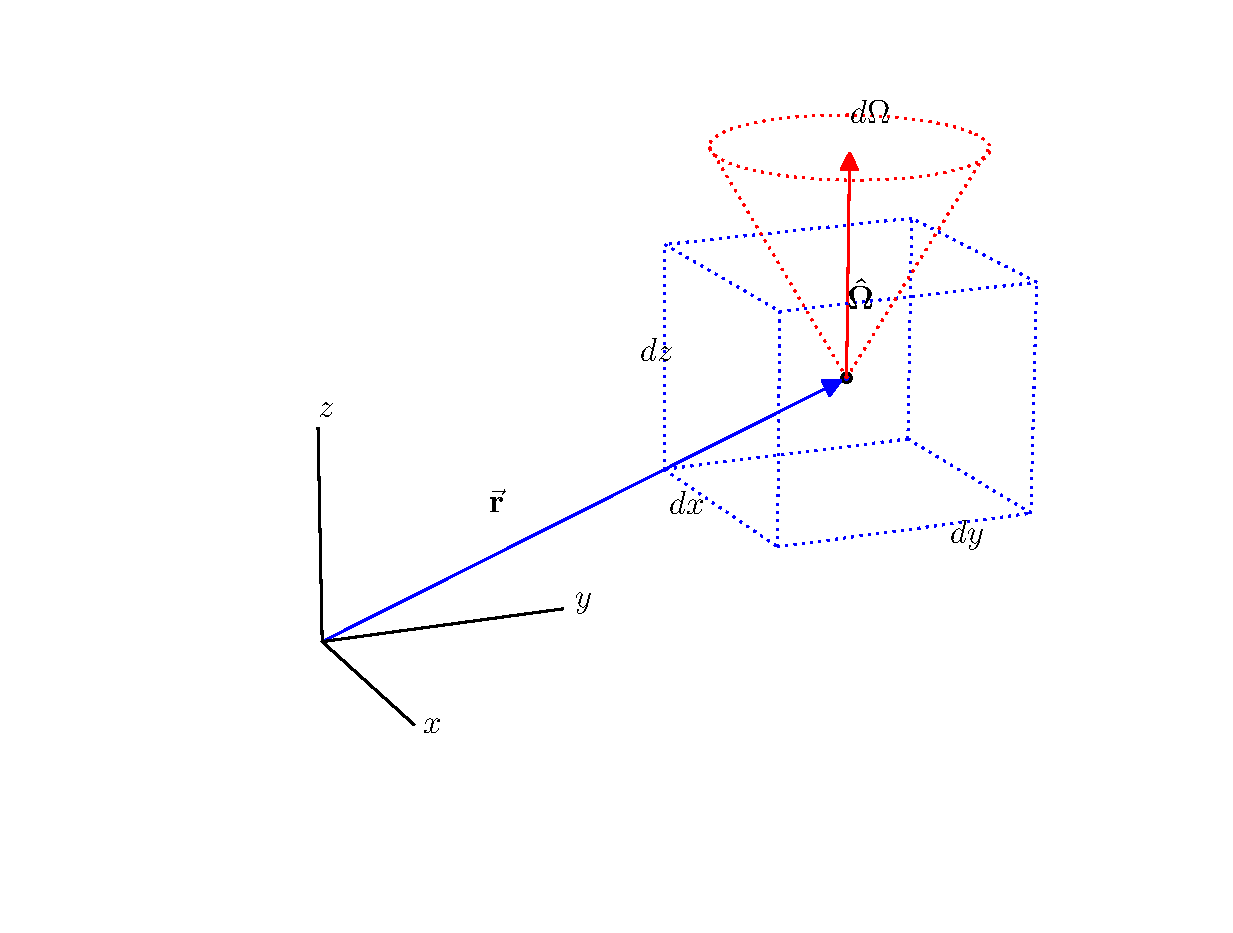
\includegraphics[width=0.8\textwidth,trim= 0cm 2.5cm 0cm 0cm]{graphics/diff_balance.eps} 
     \caption{The differential volume of the neutron balance equation. \label{diff_volume}}
\end{figure}

Before the transport equation is formulated, a neutron balance equation can be written for a differential volume.  This equation describes the amount of neutrons entering and exiting an infinitesimally-small volume, with the difference being equal to the rate of change of the neutrons within the volume.  The reactions that neutrons can undergo and how neutrons move within the material are known, so there is enough information to write such an equation.   The balance equation for the neutron density, $n$, is shown in \eqref{NBE}, and Figure \ref{diff_volume} shows an illustration of the differential volume.

\begin{equation}
\footnotesize
\begin{array}{c}
\mathrm{rate\:of\:change} = (\mathrm{production\:and\:neutrons\:in}) - (\mathrm{loss\:and\:neutrons\:out}) \\
\\
\frac{\partial n}{\partial t} = ( \mathrm{movement\:in} + \mathrm{source} + \mathrm{scatter\:in}) - ( \mathrm{movement\:out} + \mathrm{absorbtion} + \mathrm{scatter\:out})
\end{array}
\label{NBE}
\end{equation}


\subsection{Neutron Distribution Function}

The \emph{neutron distribution function}, $n(\boldsymbol{\vec{r}},\boldsymbol{\hat{\Omega}},E,t)$, 
%simply describes the number of neutrons present in each differential quantity it represents.  In the subsequent derivations, the spatial/position vector will be represented by $\boldsymbol{\vec{r}}$, the angular vector by $\boldsymbol{\hat{\Omega}}$, energy by $E$, and time by $t$.   The most detailed version of the neutron distribution function is shown in \eqref{NDF}, and is differential in space, angle, energy (or velocity), and time, and has units of the inverse of these dimensions.  In other words, it 
is the number of neutrons in volume $d\boldsymbol{\vec{r}}$ around point $\boldsymbol{\vec{r}}$, in $d \boldsymbol{\hat{\Omega}}$ around angle $\boldsymbol{\hat{\Omega}}$, $dE$ around energy $E$, and $dt$ around time $t$. 

\begin{equation}
\label{NDF}
n(\boldsymbol{\vec{r}},\boldsymbol{\hat{\Omega}},E,t) \:\: d\boldsymbol{\vec{r}} \: d \boldsymbol{\hat{\Omega}} \: dE \: dt
\end{equation}

The angle vector is a unit vector that specifies direction only, not magnitude.  It is easiest to express the directional vector as a unit vector in spherical coordinates $(\theta, \phi)$, the polar angle and the azimuthal angle, respectively.  Their Cartesian projections are given by \eqref{ang_cart} and shown in Figure \ref{ang_relations}.

\begin{equation}
\label{ang_cart}
\begin{split}
\Omega_x &= \sin \theta \sin \phi  \\
\Omega_y &= \sin \theta \cos \phi \\
\Omega_z &= \cos \theta = \mu
\end{split}
\end{equation}

\begin{figure}[h!] 
  \centering
    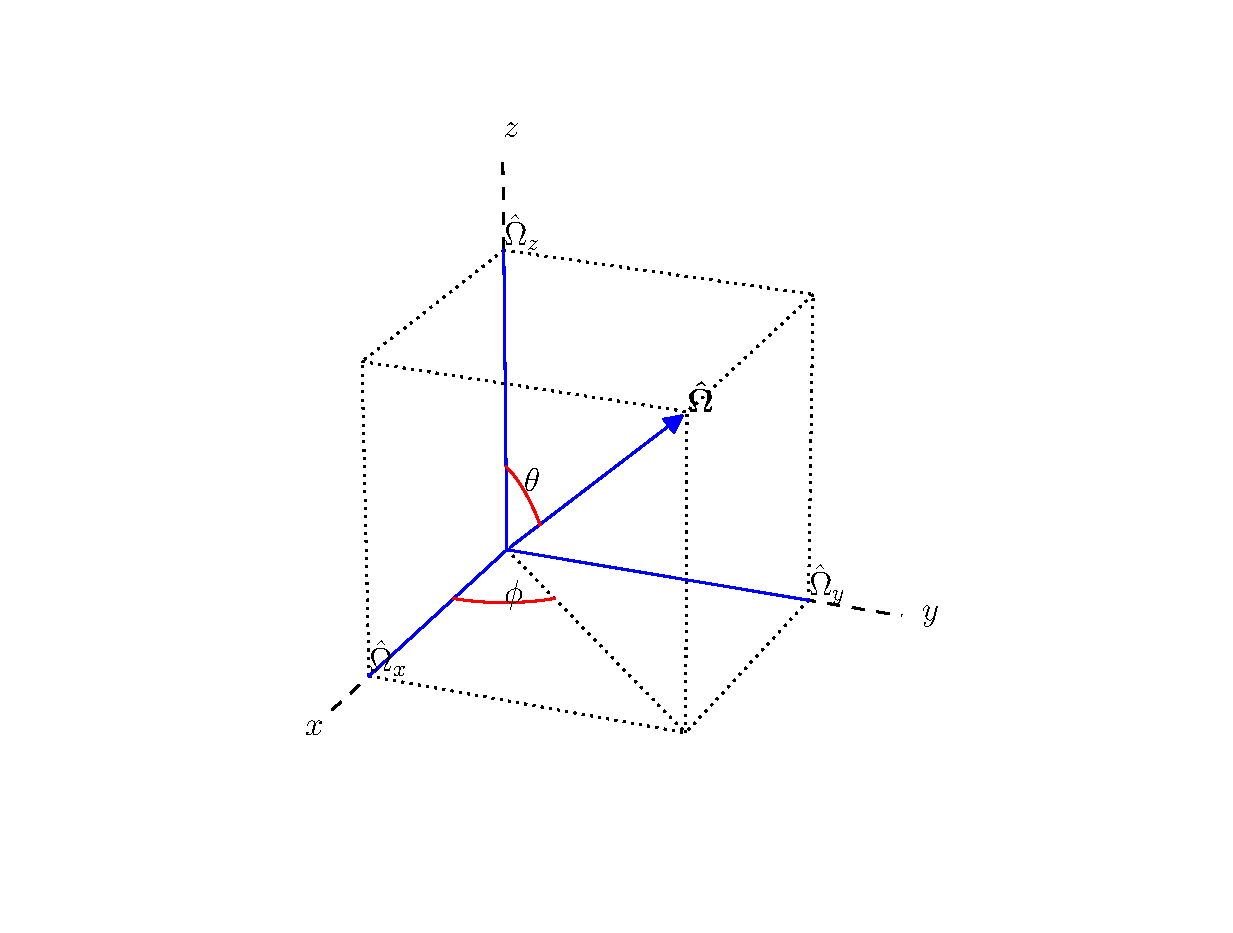
\includegraphics[width=0.8\textwidth , trim= 0cm 2.5cm 0cm 0cm]{graphics/ang_relation.eps} % trim = l b r t
     \caption{The Cartesian projections of the directional vector. \label{ang_relations}}
\end{figure}

Like any continuous distribution, it must be integrated to calculate scalar or integral quantities.  If we define the $i$th moment of the distribution according to \eqref{NDF_moments}, then the $0$th moment would be the population and the $1$st moment would be the mean if divided by the $0$th moment.

\begin{equation}
\label{NDF_moments}
M_i = \int_{-\infty}^{\infty} n(x)  x^{i} dx
\end{equation}

For example, if we are given a neutron distribution which has no time dependence, $n(\boldsymbol{\vec{r}},\boldsymbol{\hat{\Omega}},E)$, and wanted to calculate $N_V$, the total number of neutrons present in volume V, we would calculate this number by \eqref{NDF_sample}, whereas if we wanted to know the average energy, $\bar{E}$, we would do this by \eqref{NDF_avg}.

\begin{equation}
\label{NDF_sample}
N_V = \int_0^\infty dE \int_{\boldsymbol{\hat{\Omega}}} d\boldsymbol{\hat{\Omega}}  \int_{V} d\boldsymbol{\vec{r}} \: n(\boldsymbol{\vec{r}},\boldsymbol{\hat{\Omega}},E)  
\end{equation}

\begin{equation}
\label{NDF_avg}
\bar{E} = \frac{1}{N_V } \int_0^\infty dE \int_{\boldsymbol{\hat{\Omega}}} d\boldsymbol{\hat{\Omega}}  \int_{V} d\boldsymbol{\vec{r}} \: E n(\boldsymbol{\vec{r}},\boldsymbol{\hat{\Omega}},E) 
\end{equation}

\subsection{Reaction Rates}

A \emph{reaction rate} is the rate at which a certain reaction is happening in a volume \cite{duderstadt}.  If we consider a pulse-type scenario, we have $N$ particles that travel at speed $v$ in one direction.  If $\Sigma$ is the interaction probability per unit length, multiplying it by the speed gives the probability of interaction per second, or the \emph{collision rate}.  Since there are $N$ particles, multiplying the collision rate by $N$ gives the overall reaction rate, $N v \Sigma$, of the pulse in an infinite medium.  If $N$ is substituted for the neutron distribution function instead of a pulse, the expression becomes the reaction rate per distribution differential, or the \emph{reaction rate density}, $R(\boldsymbol{\vec{r}},\boldsymbol{\hat{\Omega}},E,t)$.  This expression is shown in \eqref{RR} and is the first building block of the explicit neutron balance equation.

\begin{equation}
\label{RR}
R(\boldsymbol{\vec{r}},\boldsymbol{\hat{\Omega}},E,t)  = v(E) n(\boldsymbol{\vec{r}},\boldsymbol{\hat{\Omega}},E,t) \Sigma(\boldsymbol{\vec{r}},E)
\end{equation}

If we assume there is only one energy, $E_0$ and one direction that the neutron distribution varies along, $\hat{x}$, and integrate over the other dimensions of this equation, as shown in \eqref{1d_diff}, we get an expression for the reaction rate in an infinitesimal slice, $dx$.  $A$ is the area perpendicular to the direction of motion where the neutron population is nonzero.


\begin{equation}
\label{1d_diff}
 \int_0^\infty dE \int_{\boldsymbol{\hat{\Omega}}} d\boldsymbol{\hat{\Omega}}  \int_{V} dx dy dz \:  v(E) n(\boldsymbol{\vec{r}},\boldsymbol{\hat{\Omega}},E,t) \Sigma(\boldsymbol{\vec{r}},E) \delta(E-E_0) \delta(\boldsymbol{\hat{\Omega}}-\hat{x})  = v(E_0) \Sigma(E_0) A n_{\hat{x}} (x) dx 
\end{equation}

This is effectively the loss term for a beam in the $\hat{x}$ direction, and if we set it as such, we recover the linear attenuation expression as shown in \eqref{recover_beam}, which is equivalent to \eqref{pop_diff}.  

\begin{equation}
\label{recover_beam}
dn(x) = - v \Sigma A n(x)dx  \qquad \Rightarrow \qquad  \frac{dN(x)}{dx}= - \Sigma N
\end{equation}


\subsection{Angular and Scalar Flux}

Since the reactions rate density is dependent on the cross section and the velocity multiplied by the neutron distribution, the product of just the velocity and the neutron distribution is defined as the \emph{angular flux density}, $\psi(\boldsymbol{\vec{r}},\boldsymbol{\hat{\Omega}},E,t)$,  as shown in \eqref{ang_flux}.  It is called a ``flux'' because it represents a rate at which particles are passing through a surface and ``angular'' because it is angle dependent.  Since the reaction rates depend on this quantity, the neutron transport problem is usually written in terms of the angular flux, which is then solved for instead of the neutron distribution.

\begin{equation}
\label{ang_flux}
\psi(\boldsymbol{\vec{r}},\boldsymbol{\hat{\Omega}},E,t) = v(E) n(\boldsymbol{\vec{r}},\boldsymbol{\hat{\Omega}},E,t)
\end{equation}

Scattering cross sections are differential in angle, but absorption cross sections are not, so absorption reactions can be written in terms of the \emph{scalar flux density} (or simply the \emph{flux}), which is angular flux that has been integrated over all angles.  The relation between the angular and scalar fluxes is show in \eqref{scalar_flux}.  The scalar flux is usually the most interesting quantity in reactor physics since the reactor power profile is directly proportional to it (power comes from fission, which is an absorption reaction).  The reaction rate for a reaction $i$ that has no angular dependence is shown in \eqref{scalar_flux_RR}.

\begin{equation}
\label{scalar_flux}
\phi(\boldsymbol{\vec{r}},E,t) = \int_{\boldsymbol{\hat{\Omega}}} d\boldsymbol{\hat{\Omega}} \psi(\boldsymbol{\vec{r}},\boldsymbol{\hat{\Omega}},E,t)
\end{equation}

\begin{align}
\label{scalar_flux_RR}
 R_i(\boldsymbol{\vec{r}},E,t) &= \int_{\boldsymbol{\hat{\Omega}}} d\boldsymbol{\hat{\Omega}} \: \Sigma_i(\boldsymbol{\vec{r}},E) \psi(\boldsymbol{\vec{r}},\boldsymbol{\hat{\Omega}},E,t) = \Sigma_i(\boldsymbol{\vec{r}},E) \int_{\boldsymbol{\hat{\Omega}}} d\boldsymbol{\hat{\Omega}} \: \psi(\boldsymbol{\vec{r}},\boldsymbol{\hat{\Omega}},E,t) \nonumber\\
 &= \Sigma_i(\boldsymbol{\vec{r}},E) \phi(\boldsymbol{\vec{r}},E,t)
 \end{align}
 
From \eqref{NBE} we can see that the time derivative is in terms of the neutron density, not the angular flux density.  Thus, the time dependent term must be transformed to angular flux density by multiplying and dividing it by the velocity as shown in \eqref{time_depedent_flux}.

\begin{equation}
\label{time_depedent_flux}
\frac{\partial }{\partial t}n(\boldsymbol{\vec{r}},\boldsymbol{\hat{\Omega}},E,t) = \frac{\partial }{\partial t}  \frac{v(E)}{v(E)} n(\boldsymbol{\vec{r}},\boldsymbol{\hat{\Omega}},E,t) =  \frac{\partial }{\partial t}  \frac{\psi(\boldsymbol{\vec{r}},\boldsymbol{\hat{\Omega}},E,t)}{v(E)} = \frac{1}{v(E)} \frac{\partial }{\partial t}\psi(\boldsymbol{\vec{r}},\boldsymbol{\hat{\Omega}},E,t)
\end{equation}

\subsection{Scattering}

Scattering is highly dependent on angle in addition to energy and requires a more detailed cross section expression than absorption reactions.  Elastic scattering has a fixed relation between incoming and outgoing energy and angle, but inelastic scattering does not. To be completely general in order to describe either type of scattering, all scattering cross sections are assumed to depend not only on incoming energy like all non-scattering cross sections, but also on outgoing energy, incoming angle, and outgoing angle.  Since two quantities are being related before and after the scattering event, the scattering cross section is considered \emph{doubly differential} and is sometimes called the \emph{scattering kernel}, whereas the integrated value, which only depends on incoming energy, is called the scattering cross section.   An expression for the scattering kernel is shown in \eqref{scattering_DD_xs} with the incoming values primed.
% this equality doesn't make sense to me - i think i understand what you're trying to say, but I don't understand this equation.

\begin{equation}
\label{scattering_DD_xs}
\Sigma_s = \int_{\boldsymbol{\hat{\Omega}}} d\boldsymbol{\hat{\Omega}}^\prime \int_0^\infty dE^\prime \: \: \Sigma_s(E^\prime \rightarrow E,\boldsymbol{\hat{\Omega}}^\prime \rightarrow \boldsymbol{\hat{\Omega}})
 \end{equation}

There is a practical reason for separating scattering into a cross
%use of total here is confusing
 section that describes the likelihood of a neutron entering the reaction, and a kernel that describes how it exits.  In a Monte Carlo simulation, the cross section is used to determine \emph{whether} scattering happens rather than \emph{how} it happens.  The scattering kernel is used to determine exit energy and angle only if a neutron has already been determined to scatter.  
 
This separation is also useful in expressions for scattering in a differential volume.  The cross section is used as the removal of a neutron from a particular energy and/or angle, whereas the kernel is used to determine which other energies and angles a neutron contribute to scattering \emph{into} a particular energy and/or angle.  This can be seen in \eqref{scattering_DD_xs}.  If the outgoing energy and angle are held constant, the quantity is the probability for which other angles and energies scatter into it.

Using these two quantities, in-scattering and out-scattering terms can be written for the differential volume.  The expression for loss uses the integrated cross section, shown in \eqref{scattering_loss}, and the kernel is used in what is often called the \emph{scattering source} term, shown in \eqref{scattering_source}.  The source term need to be integrated over all other energies, $E^\prime$, and angles, $\boldsymbol{\hat{\Omega}}^\prime$ from which neutrons can scatter into energy $E$ and angle $\boldsymbol{\hat{\Omega}}$.

\begin{equation}
\label{scattering_loss}
R_{s, \mathrm{out}}( \boldsymbol{\vec{r}},\boldsymbol{\hat{\Omega}},E,t ) = \Sigma_s (\boldsymbol{\vec{r}},E) \psi(\boldsymbol{\vec{r}},\boldsymbol{\hat{\Omega}},E,t)
 \end{equation}
 
 \begin{equation}
\label{scattering_source}
R_{s, \mathrm{in}}(\boldsymbol{\vec{r}},\boldsymbol{\hat{\Omega}},E,t) = \int_0^\infty dE^\prime \int_{\boldsymbol{\hat{\Omega}}} d\boldsymbol{\hat{\Omega}}^\prime \: \Sigma_s(E^\prime \rightarrow E,\boldsymbol{\hat{\Omega}}^\prime \rightarrow \boldsymbol{\hat{\Omega}}) \psi(\boldsymbol{\vec{r}},\boldsymbol{\hat{\Omega}}^\prime,E^\prime,t)  
 \end{equation}
 
 \subsection{Fission Source}

The nuclear chain reaction is sustained by fission reactions producing neutrons, so it is essential to model it in any material that has fissionable isotopes.  There are three determining factors for the fission source.  The first is the fission reaction rate, which is represented by the flux multiplied by the fission cross section.  

The second is the fission spectrum, which is represented by $\chi$.  Neutrons born from fission are not emitted at a single energy, and the fission spectrum describes the probability for a neutron to be emitted at a certain energy.  The energy spectrum is weakly dependent of the incoming neutron energy, with higher incoming energies producing more higher energy neutrons.  This dependence only starts making a significant difference in spectrum shape at energies above 10 MeV, higher than energies usually seen in a reactor.  This is why the fission spectrum is usually treated as being independent of incoming neutron energy. The spectra of $^{235}$U and $^{239}$Pu for fission induced by a 0.5 MeV neutron are shown in Figure \ref{fiss_spec}, and it can be seen that $^{239}$Pu produces more high energy neutrons.  

The last parameter is the average number of neutrons emitted in a fission event, represented by $\nu$, and is relatively flat until about 1 MeV, as was shown in Figure \ref{nu_compare}.  Since 1 MeV is within the typical energy range present in nuclear reactions, it is treated as a function of energy.

\begin{figure}[h!] 
  \centering
    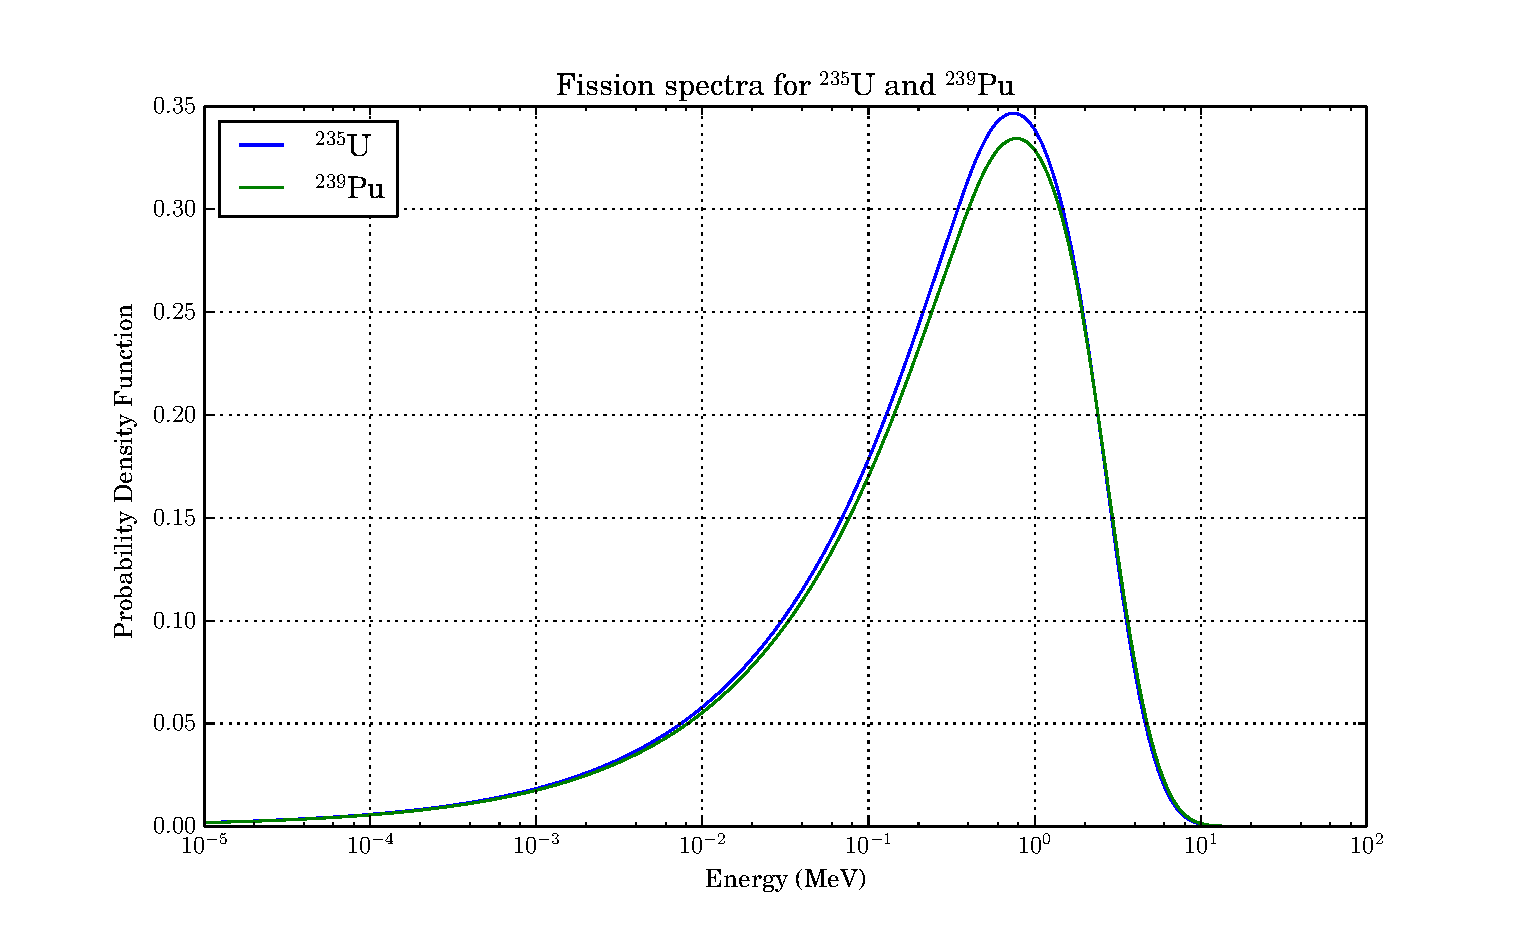
\includegraphics[width=0.8\textwidth ]{graphics/fiss_spec.eps} 
     \caption{Prompt fission neutron spectra for $^{235}$U and $^{239}$Pu. \label{fiss_spec}}
\end{figure}

The fission source term describes the number of neutrons that are born in $dE$ around energy $E$ and angle $d\boldsymbol{\hat{\Omega}}$ around $\boldsymbol{\hat{\Omega}}$ from fissions occurring from any other energy, so like the in-scattering source, the fission reaction rate must be integrated over all other energies, $E^\prime$, and angles, $\boldsymbol{\hat{\Omega}}^\prime$.  Using the general differential cross section notation and integrating the fission reaction rate over all other energies and angles yields the fission source, shown in \eqref{fiss_source1}. Multiplying by the average number of neutrons emitted in fission, $\nu$, scales the source to the proper strength.  

\begin{equation}
\label{fiss_source1}
R_f(\boldsymbol{\vec{r}},\boldsymbol{\hat{\Omega}},E,t) =  \int_0^\infty dE^\prime \int_{\boldsymbol{\hat{\Omega}}} d\boldsymbol{\hat{\Omega}}^\prime \: \nu(E^\prime) \Sigma_f(E^\prime \rightarrow E,\boldsymbol{\hat{\Omega}}^\prime \rightarrow \boldsymbol{\hat{\Omega}}) \psi(\boldsymbol{\vec{r}},\boldsymbol{\hat{\Omega}}^\prime,E^\prime,t)  
 \end{equation}
 
 Fission neutrons are born isotropically, the cross section has no incoming angular dependence, and the emission energy is very weakly dependent on incoming energy.  The angular dependence is constant and can be extracted from the differential cross section and moved outside the integral.  To keep quantities unbiased, the extracted angular distribution must integrate to one, and is therefore $1/4\pi$.  Since the emission energy does not depend on incoming energy, the fission spectrum can be extracted from the differential cross section and removed from the integral as well.  The other two fission quantities do not depend on angle, so the angular integral over angular flux density can be be replaced with the scalar flux.  The final fission source expression is shown in \eqref{fiss_source2}.

\begin{equation}
\label{fiss_source2}
\begin{split}
R_f(\boldsymbol{\vec{r}},\boldsymbol{\hat{\Omega}},E,t) & = \frac{\chi(E)}{4\pi} \int_0^\infty  \int_{\boldsymbol{\hat{\Omega}}}   \nu(E^\prime) \Sigma_f(\boldsymbol{\vec{r}},E^\prime) \psi(\boldsymbol{\vec{r}},\boldsymbol{\hat{\Omega}}^\prime,E^\prime,t) d\boldsymbol{\Omega}^\prime  dE^\prime \\
&= \frac{\chi(E)}{4\pi} \int_0^\infty   \nu(E^\prime) \Sigma_f(\boldsymbol{\vec{r}},E^\prime) \phi(\boldsymbol{\vec{r}},E^\prime,t)  dE^\prime
\end{split}
 \end{equation}
% you switched from angle integration limits of omega to 4pi. just an fyi.  oops, FIXED!


\subsection{Streaming}

So far all that has been touched on is how neutrons interact within a volume and change in angle and energy.  Now we will go over how they move in space, and to do this we consider a surface $S$ around our differential volume.  We want to find an expression for the net number of neutrons passing through this surface, and this will be our net leakage term (incoming minus outgoing).  The angular neutron flux describes the number of neutrons crossing a differential surface at angle $\boldsymbol{\hat{\Omega}}$, but in order to perform any vector operations on it, we must multiply it by the unit vector.  This new quantity is called the \emph{current density}, $\vec{\boldsymbol{J}}$, and is shown in \eqref{current}.

\begin{equation}
\label{current}
\vec{\boldsymbol{J}}(\boldsymbol{\vec{r}},\boldsymbol{\hat{\Omega}},E,t) =  \boldsymbol{\hat{\Omega}} \psi(\boldsymbol{\vec{r}},\boldsymbol{\hat{\Omega}},E,t)
\end{equation}

We can then write an expression for the leakage by performing a surface integral over the current and surface normal's dot product, shown in \eqref{leakage_surface}.

\begin{equation}
\label{leakage_surface}
\mathrm{Leakage} = \int_S ds \cdot  \vec{\boldsymbol{J}}(\boldsymbol{\vec{r}},\boldsymbol{\hat{\Omega}},E,t) = \int_S ds \cdot  \boldsymbol{\hat{\Omega}} \psi(\boldsymbol{\vec{r}},\boldsymbol{\hat{\Omega}},E,t)
\end{equation}
 
 We can turn this into a volume integral by applying the divergence theorem, shown in \eqref{div_theorem}.  If the volume of interest is shrunk to an infinitesimal volume and we switch the order of the dot product, we come to an expression that can be used in the balance equation.  This expression, shown in \eqref{streaming}, is often called the \emph{streaming} term, since it describes the net movement of neutrons into the differential volume due to their physical movement.
 
\begin{equation}
\label{div_theorem}
\int_S ds \cdot \boldsymbol{\hat{\Omega}} \psi(\boldsymbol{\vec{r}},\boldsymbol{\hat{\Omega}},E,t) = \int_V dV \nabla \cdot \boldsymbol{\hat{\Omega}}  \psi(\boldsymbol{\vec{r}},\boldsymbol{\hat{\Omega}},E,t)
\end{equation}

\begin{equation}
\label{streaming}
 \lim_{V\to dV} \int_V dV \nabla \cdot \boldsymbol{\hat{\Omega}}  \psi(\boldsymbol{\vec{r}},\boldsymbol{\hat{\Omega}},E,t) =  \boldsymbol{\hat{\Omega}}  \cdot \nabla\psi(\boldsymbol{\vec{r}},\boldsymbol{\hat{\Omega}},E,t) 
 \end{equation}
 

\subsection{Neutron Transport Equation}

Now all the terms of \eqref{NBE} have been explicitly defined.  Substituting them all in yields \eqref{NTE}, the \emph{neutron transport equation}, written here with the neutron sinks on the left side and the neutron sources on the right side.  An additional external source term, $S_{\mathrm{external}}$, has been added to account for any neutron sources not induced by the neutron flux itself, i.e.\ external sources.  This form of the equation also includes delayed neutrons.  For delayed neutron precursor group $j$, $C_j$ is the concentration, $\chi_{d,j}$ is the energy spectrum ($d$ only signifies ``delayed''), and $\lambda_j$ is the decay constant \cite{jasmina_book}.  As was stated previously, delayed neutrons are important for reactor control.  WARP is concerned with time-independent solutions, and the spectral and fission yield effects of delayed neutrons are incorporated into the data WARP uses.

\begin{equation}
\label{NTE}
\begin{split}
\frac{1}{v(E)} \frac{\partial }{\partial t}\psi(\boldsymbol{\vec{r}},\boldsymbol{\hat{\Omega}},E,t) &+  \\
\boldsymbol{\hat{\Omega}}  \cdot \nabla \psi(\boldsymbol{\vec{r}},\boldsymbol{\hat{\Omega}},E,t) &+ \\
\Sigma_t(\boldsymbol{\vec{r}},E) \psi(\boldsymbol{\vec{r}},\boldsymbol{\hat{\Omega}},E,t) & \\
& =  \\
& \quad \int_0^\infty dE^\prime \int_{\boldsymbol{\hat{\Omega}}} d\boldsymbol{\Omega}^\prime \:\: \Sigma_s(E^\prime \rightarrow E,\boldsymbol{\hat{\Omega}}^\prime \rightarrow \boldsymbol{\hat{\Omega}}) \psi(\boldsymbol{\vec{r}},\boldsymbol{\hat{\Omega}}^\prime,E^\prime,t)    \\
&+ \frac{\chi(E)}{4\pi} \int_0^\infty dE^\prime  \int_{\boldsymbol{\hat{\Omega}}} d\boldsymbol{\Omega}^\prime \:\:  \nu(E^\prime) \Sigma_f(\boldsymbol{\vec{r}},E^\prime) \psi(\boldsymbol{\vec{r}},\boldsymbol{\hat{\Omega}}^\prime,E^\prime,t)  \\
& + \sum_{j=1}^{6}\frac{\chi_{d,j}(E)}{4\pi} \lambda_j C_j(r,t)     \\
& + S_{\mathrm{external}}
\end{split}
 \end{equation}
% add delayed neutrons here
% add expression for keff here.
 
 The neutron transport equation in this form is an integro-differential equation since it has both derivates and integrals in it.  Its spatial and temporal parts are differential, whereas its angular and energy parts are integral.  It is linear and relatively easy to solve for simple geometries and reaction parameters, but in order to capture all the relevant physics for real-world problems, complex geometries and energy-dependent reaction parameters must be used.  Despite it's linearity, the neutron transport can be difficult to solve because of the large, heterogeneous domains over which it must be solved and the complex energy dependence of the cross sections.  
% the juxtaposition of the two previous sentences doesn't match. they should have the same form.  fixed??
 The energy range of interest can span more then 12 orders of magnitude, from $1\times 10 ^{-11}$ to $1\times 10 ^{1}$ MeV and above, and the geometries involved can include millions of individual material regions containing many different mixtures of materials. 
 
 \subsection{Time Independent Neutron Transport Equation}

% no longer  driven, becomes an eigenvalue problem, inf solutions, 
%From the Mats point of view, our criticality equations have infinite number of solutions, i.e. the pair of solutions: the eigenfunctions (fluxes) and corresponding eigenvalues. We are searching for the fundamental mode which corresponds to the smallest system eigenvalue (which is the largest k-eigenvalues, or our multiplication coefficient). See my slides for NE-150 on that topic (slide 32, for example).
In most situations, the equilibrium state of the neutron population is of interest.  By setting all time derivates and external sources to zero, \eqref{NTE} becomes the time-independent neutron transport equation shown in \eqref{time_ind_NTE}.  The equation is no longer driven by an independent source term, and the transport equation becomes homogenous, turning its solution into a eigenvalue problem.  There are infinitely many eigenfunction solutions to \eqref{time_ind_NTE}, and each has an associated eigenvalue.  The fundamental mode of the eigenfunction set corresponds to the longest-lived state, which is typically of greatest interested \cite{duderstadt}.  This eigenvalue is equal to the multiplication factor, which is why criticality calculations are often called ``eigenvalue'' calculations. 

In \eqref{time_ind_NTE} another parameter has been introduced, the effective multiplication factor, $k_\mathrm{eff}$, which was described earlier.  It is introduced here since, by forcing the time derivates to be zero, it is implied that the multiplication factor must be equal to one.  The physical properties of a problem may say otherwise, however, and failing to divide the fission source by the effective multiplication factor could make the time-independent equation inconsistent.  Of course there will be no inequality if the source and sink terms are actually balanced and $k_\mathrm{eff}$ calculated from \eqref{NTE} is one.  

\begin{equation}
\label{time_ind_NTE}
\begin{split}
\boldsymbol{\hat{\Omega}}  \cdot \nabla \psi(\boldsymbol{\vec{r}},\boldsymbol{\hat{\Omega}},E) &+ \\
\Sigma_t(\boldsymbol{\vec{r}},E) \psi(\boldsymbol{\vec{r}},\boldsymbol{\hat{\Omega}},E,t) & \\
& =  \\
& \quad \int_0^\infty dE^\prime   \int_{\boldsymbol{\hat{\Omega}}} d\boldsymbol{\Omega}^\prime \:\: \Sigma_s(E^\prime \rightarrow E,\boldsymbol{\hat{\Omega}}^\prime \rightarrow \boldsymbol{\hat{\Omega}}) \psi(\boldsymbol{\vec{r}},\boldsymbol{\hat{\Omega}}^\prime,E^\prime)  \\
&+ \frac{1}{k_{\mathrm{eff}}}\frac{\chi(E)}{4\pi} \int_0^\infty dE^\prime  \int_{\boldsymbol{\hat{\Omega}}}  d\boldsymbol{\Omega}^\prime \:\:  \nu(E^\prime) \Sigma_f(\boldsymbol{\vec{r}},E^\prime) \psi(\boldsymbol{\vec{r}},\boldsymbol{\hat{\Omega}}^\prime,E^\prime)  \\
\end{split}
 \end{equation}
 

%\section{Discrete Methods}

% the confluence of determinisitic and discrete methods seems a little weird to me. Frankly, I think you can just leave the whole thing out. Why mention them?
%A common strategy for solving continuous differential and integral equations on a computer is to discretize the domain over which it they are solved.  This strategy can be applied to the neutron transport equation.  Energy can be discretized by create an energy grid with set boundaries, integrating over those boundaries, and treating the reaction parameters as constant within them.  The same method can be applied to the angular dependence using an angular quadrature scheme.   The simplest way of discretizing the geometry is to voxelize the domain, laying down a  grid in each dimension and treating the material within each voxel as uniform.  The approximations introduced in each of these discretizations can cause large errors. %Discrete geometry representation is an area where irreducible error can occur since it is three dimensional and scales can range from millimeters to hundred of meters. 
% it depends on how you discretize space - I don't think you can say anything this specific. 

%Although discrete methods are readily mapped to computer hardware, often execute efficiently, and typically converge more quickly than Monte Carlo methods, there are drawbacks and limitations in using them.  The biggest drawback is that their accuracy greatly depends and the discretization methods used. For example, discretizing geometry is frequently not straight-forward. Many discrete codes use Cartesian meshes that cannot adequately capture curved surfaces. Those that use more advanced meshing strategies are plagued by the complications introduced by non-Cartesian meshes. In Monte Carlo, a sphere can be represented exactly using only its radius and the location of its center.  This matters because the amount of memory required to store the geometry and the solution can become quite large if complex geometries must be meshed finely in these discrete codes.
% I still feel a little weak about this section, but it's just my need to be super specific about discrete methods; this is fine. 

\section{Monte Carlo}
\label{sec:MC}

Deterministic methods solve the neutron transport equation directly.  They treat the neutron population as a continuous distribution and discretize the spatial, angular, energy, and temporal dimensions that the distribution depends on and solve the transport equation at these discrete points.  The Monte Carlo Method takes a different approach in mapping the transport problem to a computer.  It attempts to directly simulate what happens in reality.  Instead of the neutron population being continuous and the spatial, angular, and energy dimensions being discretized, it leaves the dimensions continuous and discretizes the neutron population.  This is how the neutrons actually exist.  They can be very well approximated by a continuous distribution, but it is still an approximation.  Quantities of interest are then determined by integrating over the neutron population.   

This way of integrating the neutron transport equation can be thought of as integrating ``sideways.''  In the Monte Carlo method, the discretized neutrons ``shoot through'' the transport equation many times, sweeping out the entire phase space, effectively integrating it when a sum is done over the individual neutron realizations, or \emph{histories}.  It is important to note that the Monte Carlo Method does not actually solve the transport equation, per se, but rather is able to \emph{estimate} the solution very well.

The Monte Carlo approach makes a physically analogous ``experiment'' on a computer.  A computer thread ``sits on top'' of a neutron as it makes a \emph{random walk} through the geometry.  The computer thread uses pseudo-random numbers to sample probability distributions that describe the interactions the neutron makes as it travels.  All the assumptions that went into deriving the neutron transport equation still hold, most importantly that neutrons travel in straight lines between interactions, that neutrons are points, and that they do not interact with each other.  The other assumption is that interactions happen instantaneously and at a point, i.e.\ they do occur over a distance.  

How surface crossing is detected in the simulation is very important since this is what changes the material data that specify the probability distributions.  WARP, in its current state, uses the traditional form of surface detection and material updates: ray tracing, the details of which will be discussed in Section \ref{sec:prelim}.  When a neutron is sampled to cross a surface, it is placed on the boundary, the material data is updated, and the interaction distance is sampled again with the neutron traveling in the same direction.  Figure \ref{random_walk} shows a cartoon of a random walk of a neutron born in the center of a cube.  The line colors represent a neutron sampling a specific material, the red ``X'' represents an absorption (walk termination), and the green ``X'' represents a surface crossing.

\begin{figure}[h!] 
  \centering
    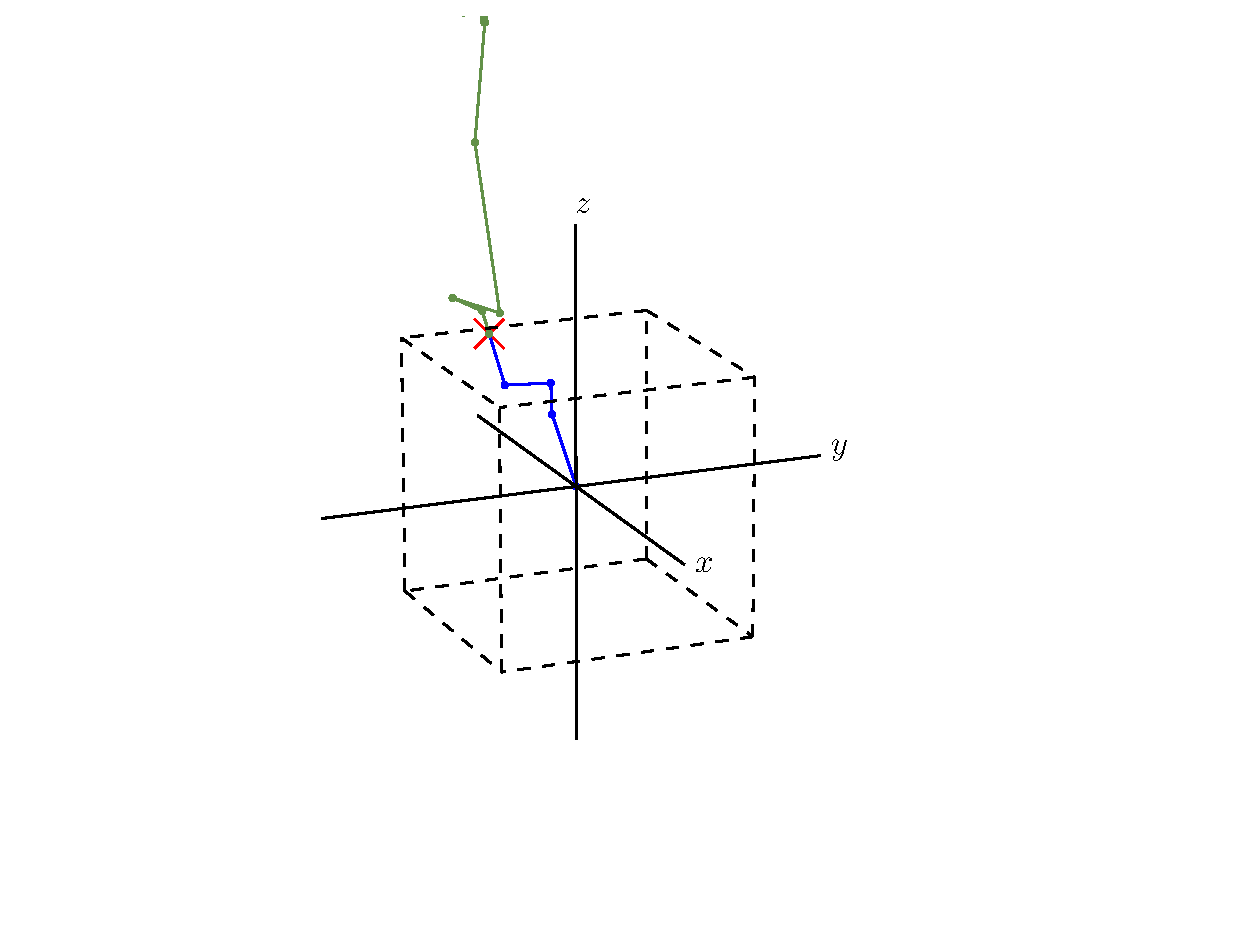
\includegraphics[width=0.8\textwidth,trim= 0cm 2.5cm 0cm 0cm]{graphics/random_walk_accepted.eps}
     \caption{The Monte Carlo random walk process. \label{random_walk}}
\end{figure}

There are advantages in using the Monte Carlo method for neutron transport, some of which have been mentioned.  The first and foremost is that very few assumptions must be made regarding the physics and the geometry of the problem. Paraphrasing Forrest Brown, the only reason people use Monte Carlo methods is that they are able to produce physically accurate results and are trusted to do so.  Anyone developing Monte Carlo code should not abuse this trust and must put accuracy first and foremost in their implementations \cite{fb_snamc}.

There are considerable drawbacks to using Monte Carlo as well; primarily convergence rates and silent inaccuracies.  Since it is a statistical calculation, it is bound by statistical laws that dictate that the error in Monte Carlo calculations reduces as $1/\sqrt{N}$, discussed in more detail in the next section, where $N$ is the number of histories performed.  The slow convergence rate can be combated by using parallel computing, however.  Requiring that neutrons do not interact with each other was an assumption that went into deriving the neutron transport equation, and can be exploited in Monte Carlo simulations.  Since each neutron history is completely independent, histories can be run completely in parallel without communication until the results are combined at the end of the simulation.  This leads to very good scaling of parallel calculations, which can be used to reduced run times of large problems to acceptable values.

A hazard associated with the statistical requirements is that very small but very influential volumes within large geometries can be missed by the neutron random walk if the number of histories is not large enough.  The estimated statistical error may be low at $N$ histories, but there is a chance the entire phase space has not yet been sufficiently sampled to produce accurate results.  
%Deterministic methods would not have this problem since there will be a discretized point in this small volume, and it will contribute to the overall calculation. % remove this sentence if you take out determ...

\subsection{Statistics}
\label{sec:stat}

To understand how the Monte Carlo Method estimates the solution to the neutron transport equation, the basics of distribution functions and statistics must be outlined.  Given a continuous random variable, $x$, that follows the probability distribution, $P(x)$, the mean value can be calculated by taking the first moment as was shown in \eqref{NDF_moments} and is reproduced in \eqref{int_mean}.  However, we are interested in determining the mean from a set samples rather than directly from the underlying distribution.  If we have $N$ independent measurements of quantity $x$, this is simply taking the arithmetic mean, as shown in \eqref{arith_mean}.  This value, computed from a finite set of measurements, $X$, is called the \emph{sample mean}, $\bar{X}$, since it is based on samples from the underlying probability distribution $P(x)$.  The \emph{true mean} is $\mu$, which is computed directly from $P(x)$.

\begin{equation}
\label{int_mean}
\mu = \int_{-\infty}^{\infty} x P(x) dx
\end{equation}

\begin{equation}
\label{arith_mean}
\bar{X} = \frac{1}{N} \sum_i^N x_i
\end{equation}

The law of large number states that the sample mean converges to the true mean in the limit where $N\rightarrow\infty$.  

\begin{equation}
\label{LLN}
Pr\left(\lim_{N\rightarrow\infty} \bar{X}_N = \mu \right) = 1
\end{equation}

The shape of the distribution of samples about the mean is important as well since it quantifies the uncertainty.  The variance can be computed by performing the central second moment on $P$, shown in \eqref{variance}. 

\begin{equation}
\label{variance}
\sigma^2 = \int_{-\infty}^{\infty} x^2 P(x) dx- \mu^2 
\end{equation}

\begin{equation}
\label{varience_est}
\mathrm{Var}(X)  =  \frac{1}{N-1} \sum_i^N (x_i-\bar{X})^2 =  \frac{1}{N-1} \left( \sum_i^N x_i^2-N\bar{X}^2 \right)
\end{equation}

Again, we are interested in determining the variance from a set samples rather than directly from the underlying distribution.  The discrete equation for computing the variance of a set of independent measurements, $X$, is shown in \eqref{varience_est}.  Dividing by $N-1$ instead of $N$ is called Bessel's Correction \cite{openmc}.  It is useful that the sample mean can be removed from the sum of the sample squares since this means that only the sample sum and the sum of sample squares need be stored.  The entire sample set does not need to be stored and used to compute the variance at the end when the sample mean is known.

The rate at which the sample mean converges to the true mean, i.e. how the uncertainty scales with the number of samples, comes from the central limit theorem.  Shown in \eqref{CLT}, the theorem states that the distribution of the means taken from a large set of independent random variables will be normally distributed \cite{openmc}.  

\begin{equation}
\label{CLT}
\sqrt{N}\left(\left(\frac{1}{N} \sum_i^N x_i \right)-\mu\right) \xrightarrow[]	{d} \mathcal{N}(0,\sigma^2)
\end{equation}

We would like to know how close the mean of such an independent set of measurements will be to the true mean.  In other words, the variance of the mean is desired.  Luckily, this can be estimated with only one measurement for the mean instead of directly computing the variance of the mean with many measurements of the mean.  The Bienaym\'e formula, shown in \eqref{bien}, states that the variance of a sum of uncorrelated random variables is equal to the sum of the variances of the variables.

\begin{equation}
\label{bien}
Var\left(\sum_{i=0}^N x_i \right) = \sum_{i=0}^N Var(x_i)
\end{equation}      

Applying the Bienaym\'e formula and the variance relation shown in \eqref{basic_var_scaling} to the sample mean results in an expression for the variance of the mean, $Var(\bar{X}_N)$, in terms of the variance of the sample, $\sigma_N^2$.  This expression is shown in \eqref{sum_var}.  

\begin{equation}
\label{basic_var_scaling}
Var\left(a X \right) = a^2 Var\left( X \right)
\end{equation}

\begin{equation}
\label{sum_var_1}
Var(\bar{X}_i) = Var\left(\frac{1}{N}\sum_{i=0}^N x_i \right) = \frac{1}{N^2} \sum_{i=0}^N Var(x_i) = \frac{N\sigma_N^2}{N^2} =  \frac{\sigma_N^2}{N} 
\end{equation}

\begin{equation}
\label{sum_var}
 \frac{\sigma_N^2}{N} = \frac{1}{N(N-1)} \left( \sum_i^N x_i^2- N\bar{X}_N^2 \right) = \frac{1}{(N-1)} \left( \frac{1}{N} \sum_i^N x_i^2 - \left(   \frac{1}{N} \sum_i^N x_i \right)   \right)
\end{equation}

It should be noted that \eqref{sum_var_1} implies that the standard deviation of the mean always scales as $1/\sqrt{N}$.  This is a blessing and a burden in that it means any calculation's variance of the mean will go to zero, i.e. the sample mean will converge to the true mean, as long it is run long enough and enough samples are collected, but that it will converge as $1/\sqrt{N}$, which is slow \cite{openmc}.

Since the central limit theorem states that the sample mean is normally distributed, we can make use of the well-know properties of the normal distribution, namely the confidence interval.  The normal distribution has well-defined confidence intervals: 68\% of the population will lie within a single standard deviation, $\sigma$, and 95.5\% will lie within $2\sigma$ \cite{jaakko}.  From this knowledge, an expression for the relative error can be written.  The expression for the relative error shown in \eqref{rel_err} is for the 68\% confidence level, and simply needs to be doubled for the 95\% level \cite{mcnp}.

\begin{equation}
\label{rel_err}
\mathrm{Rel. Err.} = \frac{\sigma}{\bar{X}_N} = \frac{1}{\bar{X}_N}\sqrt{\frac{1}{(N-1)} \left( \frac{1}{N}\sum_i^N x_i^2-\bar{X}_N^2 \right)}
\end{equation}

\subsection{Sampling Schemes}

In order to actually transport a neutron across the geometry in a Monte Carlo simulation, the probability distributions of the reaction types must be sampled to reproduce accurate distributions when the histories are aggregated.  Two methods that are commonly used are the direct inversion method and the rejection method.  

The \emph{direct inversion} method relies on being able to analytically integrate the probability distribution function (PDF) to create a cumulative distribution function (CDF) and then being able to invert that CDF.  The first step is to integrate the PDF to find the CDF, as shown in \eqref{CDF}.

\begin{equation}
\label{CDF}
CDF(x) = \int_{x_1}^{x_2} PDF(x^\prime) dx^\prime
\end{equation}
%define x_1 and x_2, done.

The bounds of integration are $x_1$ and $x_2$, which should span the entire domain of the PDF, i.e. that CDF$(x_2) - $CDF$(x_1) = 1$. Since a PDF must be positive and normalized by definition, the CDF must range from 0 to 1 and increase monotonically.  Setting the CDF equal to a uniformly distributed random number, $\xi$, and solving for the value to be sampled yields the sampling scheme.  

Figure \ref{direct_samp} shows this graphically.  The CDF describes the probability that a value of a random number, $xi$, obeying the PDF will be less than or equal to the value $x$.  Taking an integral gives the probability that $x$ will be in the interval, as shown in \eqref{CDF_property1}.  Since the width of the CDF is directly proportional to the PDF at the same value of $x$, as shown in \eqref{CDF_property2}, and if $\xi$ is uniformly distributed on [0,1), the interval $\Delta \xi$ will contain a fraction of samples on [0,1) equal to $P( x_1 < x_i < x_2)$.  As the interval width is reduced to 0, $P(x_i)= PDF(x)dx = d\xi$ (again, since $\xi$ is uniformly distributed on [0,1)), leading to the sampling scheme shown in \eqref{CDF_inversion}.  This method is only useful if the CDF is simple enough to be inverted analytically.

\begin{equation}
\label{CDF_property1}
CDF(x_2) - CDF(x_1) = P( x_1 < x_i < x_2) = \int_{x_1}^{x_2} PDF(x) dx
\end{equation}

\begin{equation}
\label{CDF_property2}
CDF(x_2) - CDF(x_1) = \Delta \xi =  \int_{x_1}^{x_2} PDF(x) dx
\end{equation}

\begin{equation}
\label{CDF_inversion}
 x_i = CDF^{-1}(\xi_i)
\end{equation}

\begin{figure}[h!] 
  \centering
    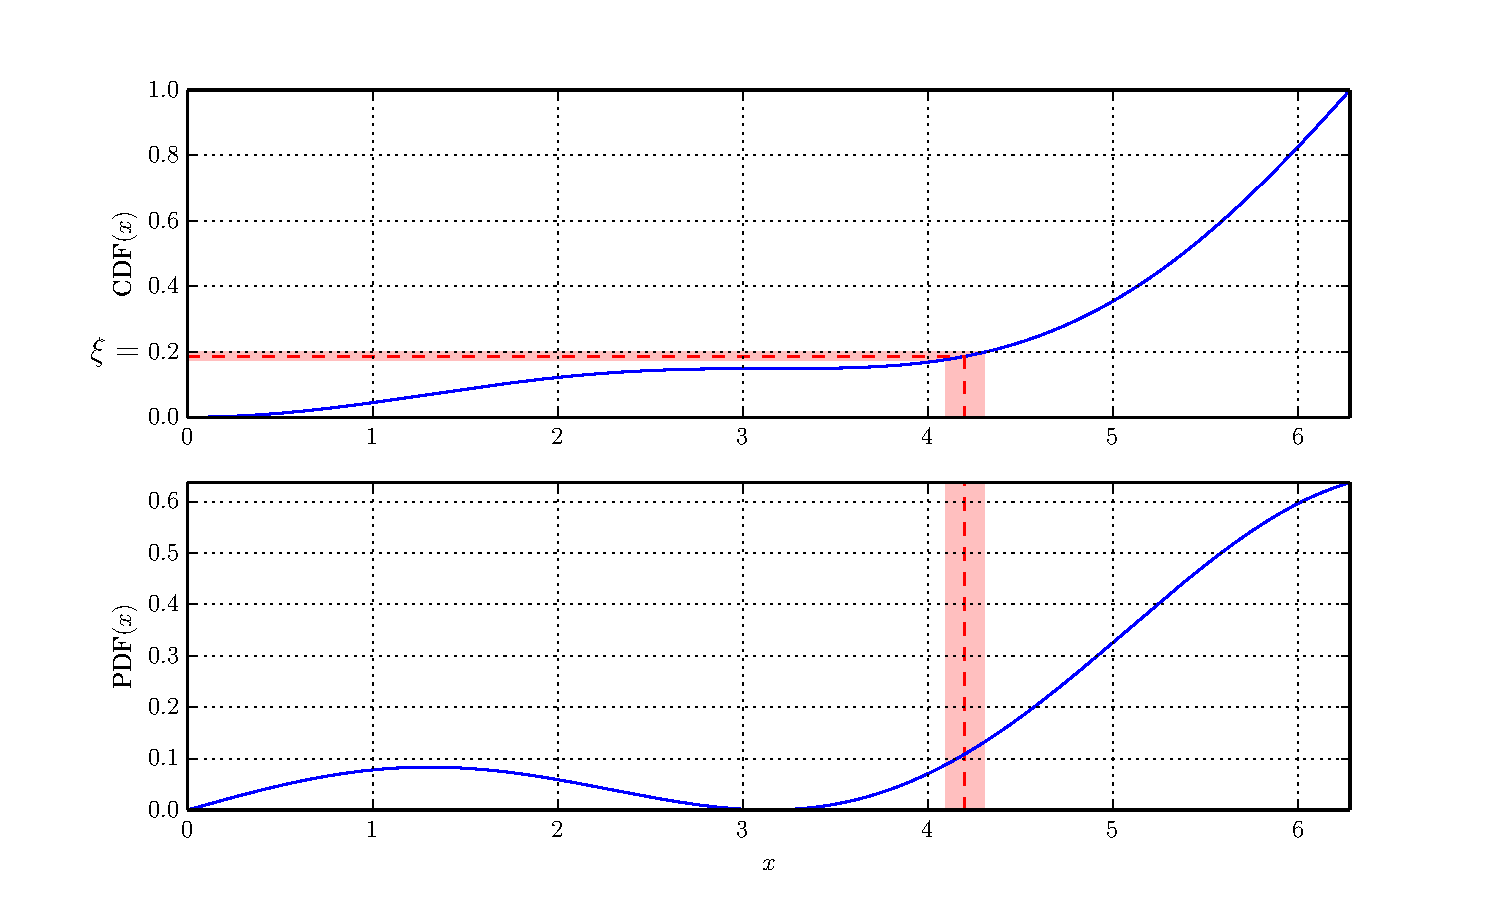
\includegraphics[width=0.8\textwidth]{graphics/direct_samp.pdf}
     \caption{Sampling $PDF(x)=\frac{1}{2\pi^2}(x \cos x - x)$ by the direct inversion method on the domain $(0,2\pi)$. \label{direct_samp}}
\end{figure}

When the CDF is not invertible, the \emph{rejection sampling} method can be used.  It uses a secondary PDF, $f(x)$, that is greater at all points in the primary PDF, $g(x)$ to be sampled from and whose CDF is easily inverted.  Since the primary PDF is normalized, $f(x)$ now corresponds to probabilities greater than one.  This is simply a scaling problem, and the random numbers used to directly sample from it must be uniform on $[0,\int_\mathrm{domain}f(x))$ instead of $[0,1)$.   Then, two random numbers are generated.  The first, $\xi_1$ is sampled from a $f(x)$ using a scaled random number as mentioned, and the second, $\xi_2$ is uniformly distributed on $[0,f(\xi_1))$.  If $\xi_2 < g(\xi_1)$, the sampled value $(\xi_1)$, is added to the population, else it is \emph{rejected}, or discarded from the population.  The set of accepted values of ${\xi_2}$ will then follow $g(x)$.  Figure \ref{rejection_samp} shows an illustration of rejection sampling. The red shaded area is the space between the primary and auxiliary PDFs where samples are rejected (red dots), and the blue shaded area is where they are accepted (blue dots).  In this illustration, the main benefit of choosing a line as the auxiliary function instead of a constant is that a line produces less red shaded area and more samples will be accepted.
%  I think I modified this to be clearer?
% explain the colors and what this means.   done.

\begin{figure}[h!] 
  \centering
    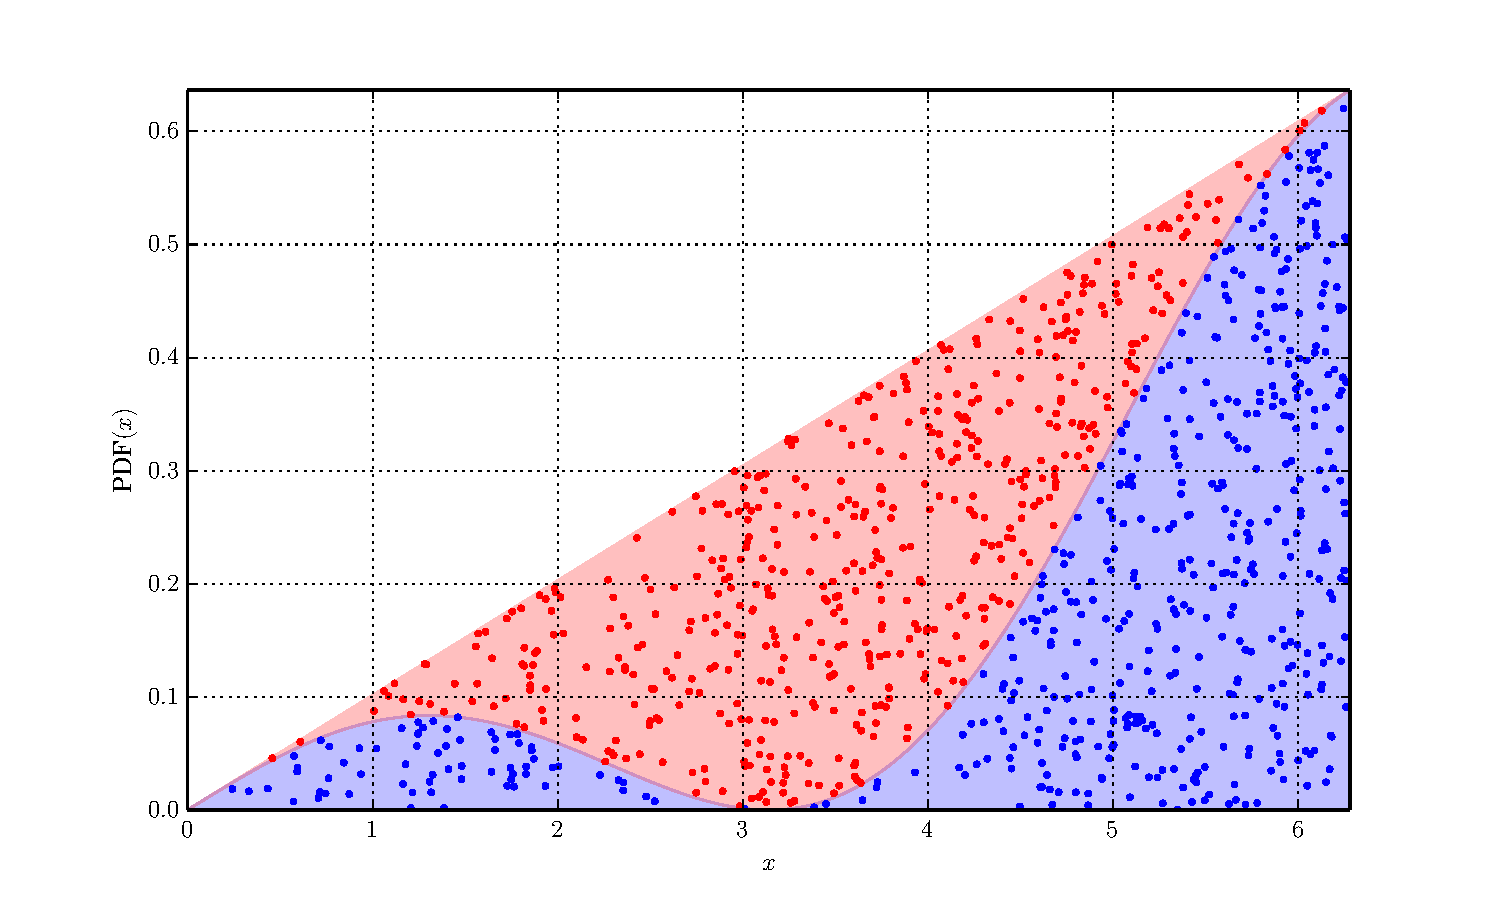
\includegraphics[width=0.8\textwidth]{graphics/rejection_samp.pdf}
     \caption{Sampling $PDF(x)=\frac{1}{2\pi^2}(x \cos x - x)$ by the rejection method on the domain $(0,2\pi)$.  The auxiliary function is $f(x)=x/\pi$ and the random number used to sample from it is uniformly distributed on $[0,2\pi)$ instead of $[0,1)$. \label{rejection_samp}}
\end{figure}

Using these two methods of sampling from probability distributions, expressions can be found for every reaction type and transport phenomenon that a neutron undergoes in its random walk through matter.  The specific schemes are described in the following subsections.

\subsubsection{Cross Section Interpolation}

When a Monte Carlo simulation is referred to as ``Continuous Energy,'' it means that the cross sections are evaluated on the fly at the exact energy the neutron is currently at instead of using a fixed value for a range of energies.  The cross section data is finite, however, and only includes data at discrete points in energy.  Therefore, interpolation must be performed between the data points to get values for any specific energy.  This is done by linear interpolation.  This assumes that the cross section is a straight line between the surrounding energy points, $E_i$ and $E_{i+1}$, and the interpolated value is calculated using the slope of the line via \eqref{xs_interp}.

 \begin{equation}
\label{xs_interp}
\begin{gathered}
E_i < E < E_{i+1} \\
\sigma(E) = \frac{E-E_i}{E_{i+1}-E_i}(\sigma(E_{i+1})-\sigma(E_i)) + \sigma(E_i)
\end{gathered}
\end{equation}



\subsubsection{Distance To Interaction}

The first step in stochastically transporting a neutron through matter is finding the distance to the next interaction.  The expression for the probability of non-interaction was shown in \eqref{pop_NI}.  The probability of interaction in $dx$ around $x$ is $\Sigma_t dx$.  Therefore the probability of not interacting from 0 to x and then interacting at $dx$ around $x$ is simply the product of these two probabilities.  The resulting expression, shown in \eqref{first_col}, is commonly referred to as the \emph{first collision probability}.
%
\begin{equation}
\label{first_col}
P(x) = \Sigma_t e^{- \Sigma_t  x}
\end{equation}
%
This expression is simple and can be inverted for direct sampling as seen in \eqref{first_col_cdf}.  The sampling scheme is shown in \eqref{first_col_samp}.  The expression $1-\xi$ can be replaced with $\xi$ since it is identically distributed.
%
\begin{equation}
\label{first_col_cdf}
CDF(x) = \int_0^x \Sigma_t e^{- \Sigma_t  x^\prime} dx^\prime = 1- e^{- \Sigma_t  x} = \xi
\end{equation}

\begin{equation}
\label{first_col_samp}
x_i=CDF^{-1}(\xi) \qquad \Rightarrow \qquad x_i=\frac{-\ln(1-\xi) }{\Sigma_t}=\frac{-\ln(\xi) }{\Sigma_t}
\end{equation}

%The total cross section $\Sigma_t$ is the total macroscopic cross section of the material the neutron is traveling through, i.e. it is the sum of the total macroscopic cross sections of its constituent isotopes as was shown in \eqref{material_sum_xs}.
% unnecessary at this point

\subsubsection{Isotope and Reaction Selection}

Once a neutron has been determined to interact, the isotope with which it interacts must be decided.  The discrete PDF of this process is shown in \eqref{isotope_selection}, where there are $i$ isotopes in the material each having a total macroscopic cross section $\Sigma_{t,i}$.  The distribution is sampled by generating a uniform random number, $\xi_1$, on $[0,1)$ and performing a running sum over the individual isotope's total macroscopic cross sections.  When $CDF_i > \xi_1$, the neutron collision is sampled to happen in isotope $i$.

\begin{equation}
\label{isotope_selection}
PDF_i = \frac{\Sigma_{t,i}}{\Sigma_t} \qquad \Rightarrow \qquad CDF_i = \frac{1}{\Sigma_t } \sum_{n=1}^i \Sigma_{t,n}
\end{equation}

Determining the reaction type is done in a similar fashion, except the number density of the material is no longer a concern since the isotope has already been selected.  Therefore, the running sum of the CDF is done over isotope $i$'s microscopic cross sections.  Another random number is generated, and when $CDF_k > \xi_2$, the neutron is sampled to undergo reaction $k$ in isotope $i$.

\begin{equation}
\label{reaction_selection}
PDF_k = \frac{\sigma_k}{\sigma_t} \qquad \Rightarrow \qquad CDF_k = \frac{1}{\sigma_{t} } \sum_{n=1}^k \sigma_{n}
\end{equation}


\subsubsection{Tabular Distribution Interpolation}

For reactions that have exiting neutrons, like scattering and fission, there are probability tables containing CDFs that specify at what probability neutrons will be emitted with certain angles and energies.  To sample from these tabular CDFs, a random number, $\xi$, is generated.  Again, since the data is discrete, some type of interpolation must be performed to generate a value between the data points.  

There are two interpolation methods specified in the ENDF format.  The first is histogram interpolation, which is similar to the linear cross section in the previous section.  Histogram interpolation assumes the CDF is a line between the data points, and the interpolated value is calculated to lie on this line.  Since the CDF is the integral of the PDF, assuming the CDF is a line is the same as assuming the PDF is a constant, i.e. the PDF is a histogram.  The data for the histogram could be obtained from using a tabulated PDF that is typically provided to compute the CDF.  Using the PDF data is unnecessary, however, since these values can be computed from the CDF and this approach reduces the global memory access of a GPU kernel. 
% I think what I wrote makes sense? fix it if it's not. what you had before was confusing...

An example of using histogram interpolation to determine outgoing cosine, $\mu^\prime$, is shown in \eqref{histo_interp}, where $C_{i}$ is the value of the CDF at point $i$ and $P_i$ is the value of the PDF at point $i$.  $\mu^\prime_i$ represents the corresponding value of $\mu^\prime$ in the table at point $i$ \cite{openmc}.
  While this example is for $\mu^\prime$, this method can be used to sampled a CDF of any quantity.

 \begin{equation}
\label{histo_interp}
\begin{gathered}
C_i < \xi < C_{i+1} \\
 \mu^\prime(\xi) = \frac{\xi-C_i}{C_{i+1}-C_i}(\mu^\prime_{i+1}-\mu^\prime_i) + \mu^\prime_i
\end{gathered}
\end{equation}

The second method is called linear-linear interpolation.  Instead of assuming the PDF is constant between the tabular points (and CDF is linear), it assumes the first derivative (the PDF) is linear over the interval $C_i < \xi < C_{i+1}$.  The linear expression for the PDF as in \eqref{lin_pdf} is substituted into \eqref{CDF_property1} and integrated to $\mu^\prime$.  Again this derivation is shown for $\mu^\prime$, but is valid for any CDF \cite{openmc}.
% adding these to make this all one paragraph.
\begin{equation}
\label{lin_pdf}
\begin{gathered}
C_i < \xi < C_{i+1} \\
P(\mu^\prime) = \frac{P_{i+1}-P_i}{\mu^\prime_{i+1}-\mu^\prime_i}(\mu^\prime - \mu^\prime_i) + P_i = a \mu^\prime + b
\end{gathered}
\end{equation}
%
Integration of \eqref{lin_pdf} to $\mu^\prime$ yields \eqref{lin_pdf_int}.  This expression for $CDF(\mu^\prime)$ is set equal to the random number $\xi$ and solved for $\mu^\prime$ to give the interpolation function.
%
\begin{equation}
\label{lin_pdf_int}
C(\mu^\prime) = C_i  + \int_i^{\mu^\prime} P(\mu^{\prime\prime}) d\mu^{\prime\prime}  =  C_i  + \int_i^{\mu^\prime} \left( a \mu^{\prime\prime} + b \right) d\mu^{\prime\prime} = C_i  + \frac{a}{2}(\mu^{\prime 2}-\mu^{\prime 2}_i) + b(\mu^\prime-\mu^\prime_i) = \xi 
\end{equation}
% What does the lower bound of i mean, and why does \mu_i get integrated as well? I thought that was a fixed value? 
\eqref{lin_pdf_int} can be solved for $\mu^\prime$, yielding \eqref{lin_lin}, the final form of the linear-linear sampling scheme \cite{openmc}.
%
\begin{equation}
\label{lin_lin}
\begin{gathered}
a = \frac{P_{i+1}-P_i}{\mu^\prime_{i+1}-\mu^\prime_i} \qquad , \qquad b = P_i - a \mu^\prime_i \\
\mu^\prime = \mu_i + \frac{1}{a}\left( \sqrt{P^2_i + 2a(\xi -C_i)} -P_i \right)
\end{gathered}
\end{equation}
% I don't quite understand the equation progression here. I'd write the definition of a and b as part of lin_pdf since you establish this relationship already and it will make the leap from lin_pdf_int to lin_lin clearer. I also don't understand lin_pdf_int result.

Each tabular distribution in the ACE data file specifies if the histogram or linear-linear method should be used to perform interpolation on it.  It is not up to the user to decide what scheme to use if results consistent with Serpent or MCNP are desired.  The CDFs are tabulated with the specified interpolation method in mind, and using the incorrect scheme will produce incorrect results.  The interpolation scheme must be checked for each distribution on a case-by-case basis. 
% what does this mean? is it because of what data is available? what you're trying to do? what's most accurate? 

\subsubsection{Free Gas Treatment}

As stated previously, the data in the cross section libraries are Doppler broadened for a certain material temperature.  This is done to account for the effect the target nuclei's thermal motion has on the apparent width of resonances when the target nuclides are modeled as stationary. As a result, Doppler broadening produces accurate reaction rates in the resonance region when target nuclides are modeled to be stationary, and modeling the targets as stationary is a good approximation when the neutron velocities in the resonance region. 

However, a stationary target model would incorrectly allow a neutron to scatter down to absolute zero.  In reality, they scatter until they come into thermal equilibrium with the target nuclides.  Once they are in equilibrium, on average they lose the same amount of energy as they gain from scattering events and their population becomes stationary in energy.  To preserve this collection phenomena, or \emph{thermal peak}, in Monte Carlo simulations, the velocity of the target nuclide must be explicitly modeled.  

%Elastic scattering is the only interaction that has a neutron at thermal energies in the exit channel, and therefore is the only reaction that needs to consider target velocity.  Fission produces secondary neutrons in distributions uncorrelated with incoming neutron energy or target velocity at thermal energies, so the target motion can be disregarded.  Since the Doppler-broadened cross sections produce accurate reaction rates when the targets are modeled to be stationary, this quantity must be preserved when giving the targets a nonzero velocity.  
% you might not need this paragraph anymore

The targets follow a Maxwell-Boltzmann speed distribution, but this cannot be sampled directly for simulation purposes because of the Doppler broadening preprocessing done to the cross section data.  Near resonances, portions of the thermal distribution within the resonance contribute much more to the overall reaction rate than the portions outside of it.  Directly sampling a target velocity from the thermal distribution would produce incorrect exiting neutron energies.  Rather, the distribution of target velocities that contributed to the reaction rate (and therefore the thermally averaged cross section) must be calculated and sampled from.

Elastic scattering is the only interaction that has a neutron at thermal energies in the exit channel, and therefore the only use for the target velocity is in scattering kinematics to reproduce an accurate thermal peak while maintaining reaction rates.  For the sake of completeness, the following derivation is included and closely follows that in \cite{openmc} and \cite{gelbard}.  The reaction rate in terms of the target and neutron velocities is shown in \eqref{RR_vel} and is equivalent to \eqref{broaden} in Section \ref{sec:temp}.

\begin{equation}
\label{RR_vel}
R (\boldsymbol{v_t}) = ||\boldsymbol{v_n}-\boldsymbol{v_t}|| \sigma(||\boldsymbol{v_n}-\boldsymbol{v_t}||) M(v_t)
\end{equation}

Since elastic scattering is the only reaction of interest, $\sigma(v_\mathrm{rel})$ can be assumed to be constant.  This assumption is good for most nuclides since the elastic cross sections are in fact relatively constant at low energies.  If there is a low-energy scattering resonance, this approximation may produce results that skew the distribution towards lower energies \cite{openmc}, but it is good for most nuclides.  

Substituting the Maxwell-Boltzmann speed distribution for $M(v_t)$, the simplified PDF for target velocities can be written as \eqref{RR_vel_simp} where $C$ is the normalization constant calculated from \eqref{RR_vel} and $m$ is the mass of the target nucleus.
% there's no $C$ in \eqref{RR_vel} ?    added to eq.
%
\begin{equation}
\label{RR_vel_simp}
\begin{gathered}
C = \int_0^\infty d\boldsymbol{v_t} \:\: R(\boldsymbol{v_t}) \\
\beta = \sqrt{\frac{m}{2kT}} \\
PDF(\boldsymbol{v_t}) = C v_\mathrm{rel} \sigma \left[   \frac{4}{\sqrt{\pi}} \beta^3 v_T^2  \exp (- \beta^2  v_T^2 )      \right]
\end{gathered}
\end{equation}
% define m. done.
Applying the law of cosines to $v_\mathrm{rel} = ||\boldsymbol{v_n}-\boldsymbol{v_t}||$ yields \eqref{RR_vel_expanded}, which has changed from a vector equation to a scalar one.   The new PDF has two unknowns, the target velocity $v_T$ and the angle between it and the neutron velocity, $\mu$.

\begin{equation}
\label{RR_vel_expanded}
\begin{gathered}
\beta = \sqrt{\frac{m}{2kT}} \\
PDF(v_t) = C \sigma  \sqrt{v_n^2+v_t^2-2 v_n v_t \mu} \left[   \frac{4}{\sqrt{\pi}} \beta^3 v_T^2  \exp ( -\beta^2  v_T^2 )      \right]
\end{gathered}
\end{equation}

Note that there is a restriction on $\mu$.  There cannot be cases where sampled values of $\mu$ and $v_T$ produce a negative $v_\mathrm{rel}$, which corresponds to the target neutron ``running away'' from the incident neutron.  Such a case is non-physical since it would imply that the reaction never happened.  This is the first reason why rejection sampling is needed to determine an appropriate target velocity.  The PDF in \eqref{RR_vel_expanded} is sampled and the velocity is rejected if it violates the restriction on $\mu$. % does this translate into math that you use? If so, add it. If not, you probably don't need this paragraph?  Yes, this is the reason rejections sampling is needed, otherwise it could be directly inverted.

The second reason rejection sampling is used is that the PDF in \eqref{RR_vel_expanded} cannot be directly inverted.  However, it can be split into two PDFs, $f_1(v_T)$ and $f_2(v_T)$ as seen in \eqref{RR_vel_split}, which can be inverted.  Sampling from the product of two invertible functions is possible by rejection.  The sampling scheme for this is to normalize $f_2(v_T)$ (so its integral is one) and sample from it directly.  The sample from $f_2(v_T)$ is accepted based on the probability in \eqref{RR_vel_split_samp} \cite{openmc}.
% these last two sentences are not so clear.
The multiplication and division by $v_n^2+v_t^2$ seen in \eqref{RR_vel_split} guarantees that $f_1$ is bounded between 0 and 1.  This is necessary since $v_\mathrm{rel}$ is not bounded in any way.  The normalization using $f_2$ to make ``$CDF(v_T)$" is expanded and simplified in \eqref{RR_vel_split_norm}, where $y=\beta v_n$ and $x=\beta v_t$.  The acceptance probability of the sample is shown in \eqref{RR_vel_split_accept}

\begin{equation}
\label{RR_vel_split}
\begin{gathered}
f_1(v_T,\mu) = C \sigma  \frac{\sqrt{v_n^2+v_t^2-2 v_n v_t \mu}}{v_n^2+v_t^2}\\
f_2(v_T) =  \frac{4}{\sqrt{\pi}} (v_n^2+v_t^2) \beta^3 v_T^2  \exp ( -\beta^2  v_T^2 )
\end{gathered}
\end{equation}

\begin{equation}
\label{RR_vel_split_samp}
``CDF(v_T)" = \frac{f_2(v_T)}{\int f_2(v_T)} \qquad \Rightarrow \qquad v_T^\prime 
\end{equation}

\begin{equation}
\label{RR_vel_split_accept}
p_\mathrm{accept} = \frac{f_1(v_T^\prime,\mu)}{ f_1(v_T^\prime,\mu=0)}
\end{equation}
% I'd put the cdf terms all together and make the acceptance probability separate.

\begin{equation}
\label{RR_vel_split_norm}
\begin{split}
``CDF(v_T)" &=  \frac{f_2(v_T)}{\int f_2(v_T)} = \frac{  (v_n^2+v_t^2) \beta^3 v_T^2  \exp ( -\beta^2  v_T^2 ) }{ \frac{1}{4\beta} \sqrt{\pi} \beta v_n +2 } \\
&= \left( \frac{4}{\sqrt{\pi}}  \frac{\sqrt{\pi}y}{\sqrt{\pi}y+2} \right) x^2 \exp(-x^2)  + \left( 2  \frac{2}{\sqrt{\pi}y+2} \right) x^3 \exp(-x^2) \\
\end{split}
\end{equation}

Since this CDF is the weighted sum of two independent distributions, the combined PDF can be sampled by sampling the second term with a probability of $2/(\sqrt{\pi}y+2)$ and the first term otherwise.  % explain this more clearly. Are the two distributions independent? Why are we sampling them separately? don't you need both terms to get the CDF?  Is this better?
While both distributions appear complicated, each can be directly sampled via the schemes C49 and C61 provided in the Third Monte Carlo Sampler manual \cite{3rdsampler}.  Sampling scheme C49, shown in \eqref{C49}, is for sampling distributions of the form $\nu^{2n-1}e^{-\nu^2}$ where $n$ is an integer $\ge 1$ and $\nu$ is a continuous random variable, i.e.\ for Gaussians multiplied by variables of odd powers.  This is scheme is appropriate for sampling a value of $x^\prime$ from the second term in \eqref{RR_vel_split_norm} when $n=2$, and is shown in \eqref{C49_x}.

\begin{equation}
\label{C49}
\nu = \sqrt{- \ln \left( \prod_{i=1}^n \xi_i \right) } 
\end{equation}

\begin{equation}
\label{C49_x}
 x^\prime = \sqrt{- \ln \left( \xi_1 \xi_2 \right)}
\end{equation}

% what are \nu and x'? how are they used? You don't need to re-tell us that n=2  done.

Sampling scheme C61, shown in \eqref{C61}, is for expressions of the for $\nu^{2n-1}e^{-\nu^2}$ where $n$ is a half integer $\ge 1/2$, i.e.\ for Gaussians multiplied by variables of even powers.  When $n=3/2$, this is a sampling scheme for the first term in \eqref{RR_vel_split_norm}, and is shown in \eqref{C61_x}.

\begin{equation}
\label{C61}
\begin{gathered}
h = n-1/2 \\
\nu = \sqrt{- \ln \left( \prod_{i=1}^h \xi_i  \right)+ \tau^2} \\ 
\tau^2 = -\ln(\xi_1) \cos^2(\frac{\pi}{2}\xi_2)\\
\end{gathered}
\end{equation}

\begin{equation}
\label{C61_x}
x^\prime =   \sqrt{- \ln( \xi_1) - \ln(\xi_2) \cos^2(\frac{\pi}{2}\xi_3)}
\end{equation}

% same questions about what this is.  Better?

After the first or second term of \eqref{RR_vel_split_norm} is sampled (RHS sampled with probability $2/(\sqrt{\pi}y+2)$) to give $x^\prime$, it can be transformed to $v_T^\prime$ via $v_T^\prime=x^\prime/\beta$.  Once a value for $v_T^\prime$ is determined, it must be accepted or rejected based on the angular constraint imposed by the rejection criterion \eqref{RR_vel_split_accept}.  The rejection criterion requires a value for $\mu^\prime$, however.  Since this is for a thermal distribution, $\mu$ is sampled isotropically as shown in \eqref{mu_samp}.  Once $\mu$ is sampled, $f_1(v_T,\mu)$ can be calculated, and the sampled values of $v_T^\prime$ and $\mu$ are accepted with the probability $p_\mathrm{accept}$ as shown in \eqref{prob_accept}, i.e.\ the values are accepted if random number $\xi$ satisfies $\xi<p_\mathrm{accept}$.  If the sample is rejected, the whole process is repeated until a pair of $v_T^\prime$ and $\mu$ are accepted.  
% make sure the above is clear, is it now?


\begin{equation}
\label{mu_samp}
\mu = 2\xi - 1 
\end{equation}

\begin{equation}
\label{prob_accept}
p_\mathrm{accept} = \frac{\sqrt{v_n^2+v_t^2-2 v_n v_t \mu}}{v_n^2+v_t^2}
\end{equation}

Even though this is a rejection method, it is fairly efficient, with samples being accepted 68\% up to 100\% of the time as the neutron velocity either goes from zero to values much greater than the target velocity \cite{mcnp}.

\subsubsection{Stochastic Mixing}

The ENDF data tables have probability distributions for reactions at discrete energy points, but this is not physically accurate.  The reactions do not abruptly transition from one PDF to another at a single energy, they smoothly transition.  This is why \emph{stochastic mixing} is prescribed in the ENDF tables.  If the neutron energy, $E$, falls between the ENDF data energy grid values $i$ and $i+1$, the neutron will use data from table $i+1$ with probability $f$, defined in \eqref{mixing_prob} \cite{openmc}.
%
\begin{equation}
\label{mixing_prob}
\begin{gathered}
E_i < E < E_{i+1} \\
f = \frac{E-E_i}{E_{i+1}-E_i}
\end{gathered}
\end{equation}
%
As $E$ approaches $E_{i+1}$, the probability it will sample from the $i+1$ distribution goes to 1 linearly.  This ensures smooth transitions between reaction data tables.

\subsubsection{Elastic Scattering}

The kinematics of elastic scattering were outlined in Section \ref{subsec:interactions}, and even though it seems only the velocities and masses of the target and neutron are needed, data tables still need to be queried to carry out the interaction.  At energies below the MeV range, elastic scattering is isotropic in the CM frame, but at these energies and above, it becomes significantly anisotropic.  Figure \ref{scattering_anisotropy} shows this in $^{16}$O.  At high energies, the scattering is both forward- and backward-peaked.  

\begin{figure}[h!] 
  \centering
    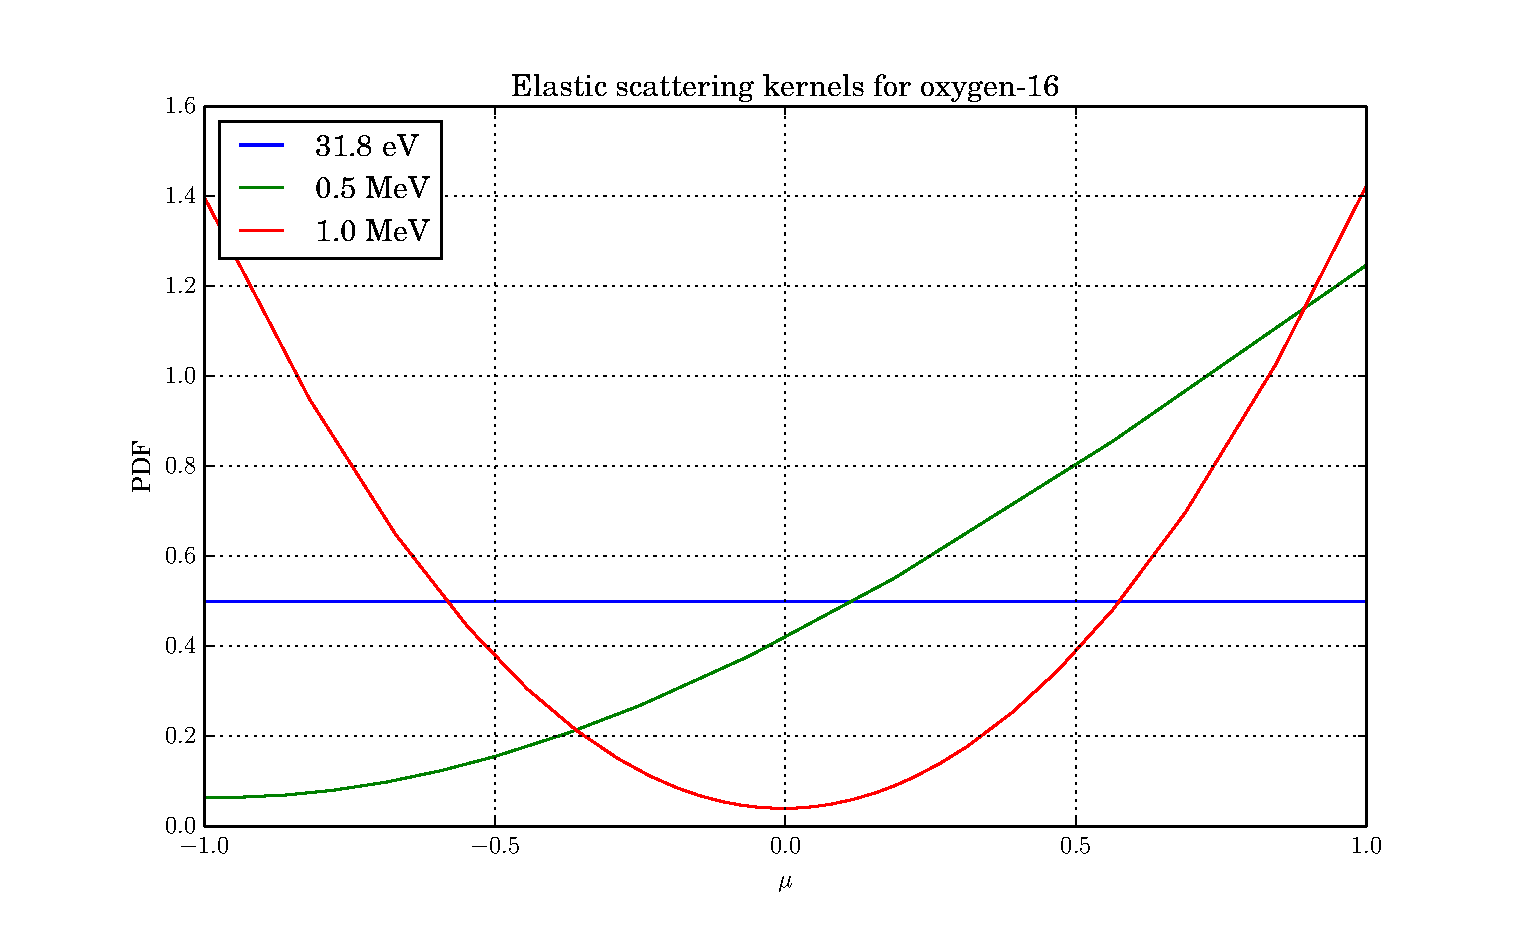
\includegraphics[width=0.8\textwidth]{graphics/scattering_anisotropy.eps}
     \caption{Elastic scattering anisotropy at high energies in $^{16}$O.  \label{scattering_anisotropy}}
\end{figure}

It is essential to model this phenomena accurately since the scattering angle factors heavily into the energy exchange between the particles.  Figure \ref{scattering_error} shows what can happen when elastic scattering is treated as isotropic for all energies.  The figure shows the normalized flux per unit lethargy in a one meter cube of water with a 2 MeV point source at its center as calculated by WARP (red) and by Serpent (blue).  The neutron flux spectra at scattering resonances (which are apparent at 0.32, 1.0, and 1.2 MeV from the sharp dips in the flux) is too small, and the flux immediately after the resonances is too large.   

\begin{figure}[h!] 
  \centering
    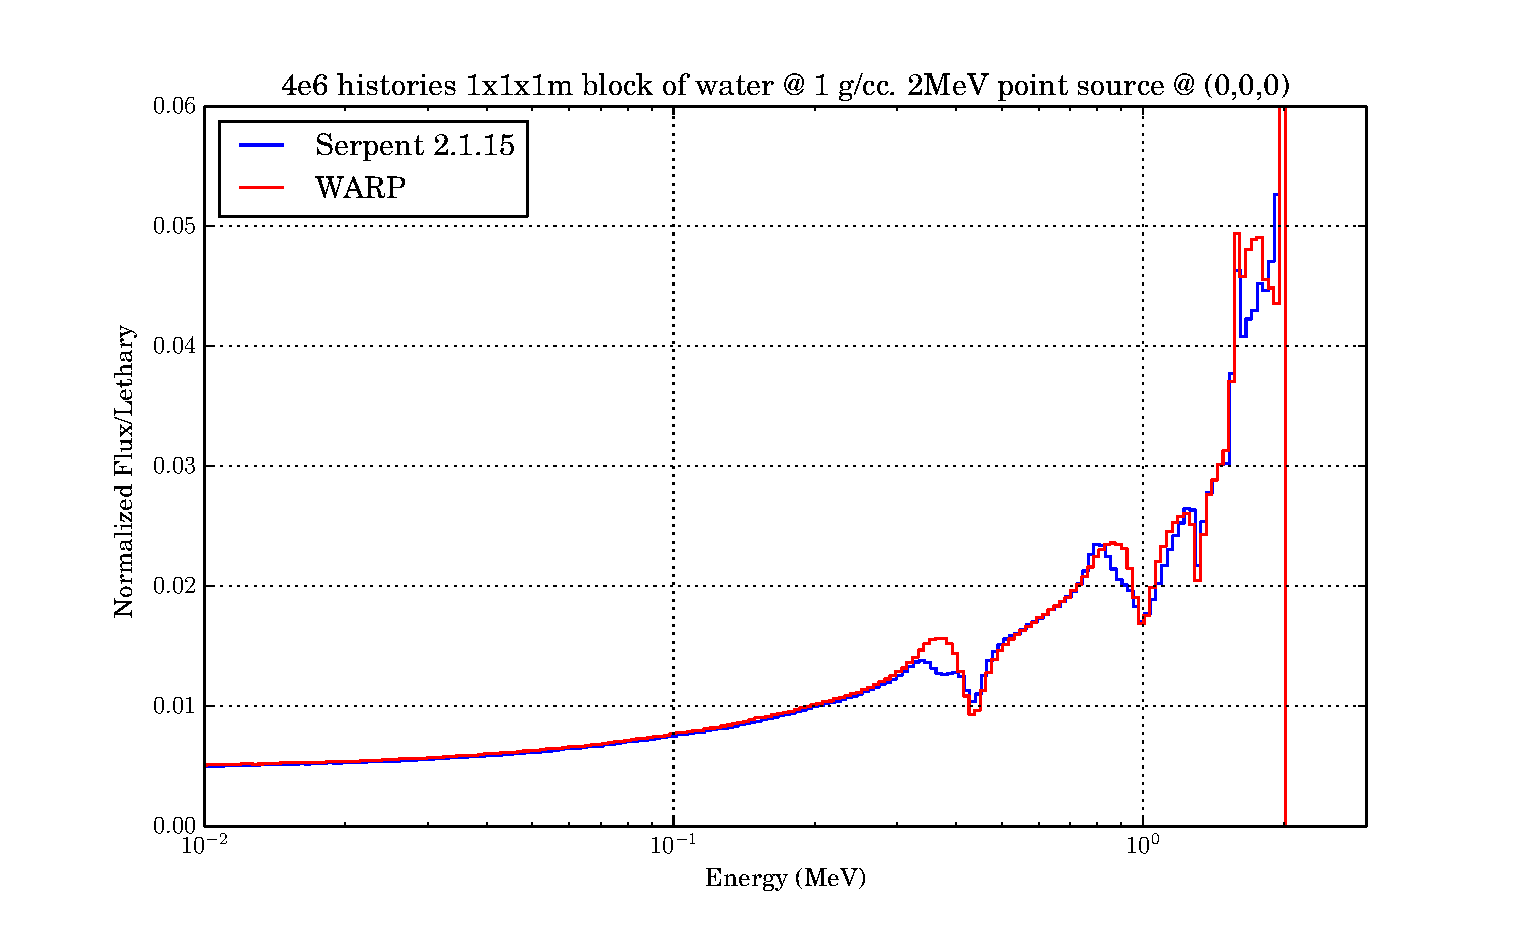
\includegraphics[width=0.8\textwidth]{graphics/scattering_error.eps}
     \caption{An inaccurate flux spectrum produced by WARP compared to a correct one from Serpent highlighting the errors caused by treating elastic scattering as isotropic for all energies.\label{scattering_error}}
\end{figure}
% This isn't a plot of error, it's a plot of flux.  FIXED.

The anisotropy shown in \ref{scattering_anisotropy} at the 1 MeV resonance indicates that a neutron should either lose a little (forward-peaked elastic scattering) or a large (backward-peaked elastic scattering) amount of energy in the elastic scattering event.  It should not lose an intermediate amount.  The minimum fraction of energy than can be lost to $^{16}$O is zero and the maximum is $1-((16+1)/(16-1))^2=0.22$ \cite{duderstadt}.  The errors shown in Figure \ref{scattering_error} typically span 2 octaves in the logarithmic flux plots, which is consistent with the maximum factional energy loss.  In the completely isotropic flux, the higher flux at intermediate energies indicates that neutrons are being scattered to these energies at a higher rate than Serpent.  It is low immediately on the resonance because neutrons are leaving the energy bin faster than they should be and are not scattering multiple times within the bin (as they would if they lost no energy in the elastic scattering event).  

The point of highlighting this phenomenon is that sampling angular dependence of the scattering kernels is very important for obtaining correct results, especially for elastic scattering where the energy exchange are completely defined by the scattering angle and the target momentum.  The energy dependencies cannot be ignored and the distributions specified in the nuclear data must be sampled as specified in the data tables.  Elastic scattering is very common (and often dominant) reaction and modeling it accurately is essential to obtaining correct results.
% how do you know that? do you have a reference? how are you deciding what is wrong? we also don't know where the resonances are...
% okay, how does this relate to the previous sentence? and the point you're making here?
% does it make more sense now?   I need to make a point here unless i just want to say refer to section 2.2
WARP used the tabular CDF format to sample the outgoing CM angle of the neutron in elastic scattering, which normally uses histogram interpolation.  The process is as follows:    
\begin{enumerate}
 \item The neutron energy and direction are converted to velocity.
 \item The target velocity is sampled as described in the previous subsection.
 \item The center of mass velocity is calculated and the neutron and target velocities are transformed to the CM frame.
 \item The polar scattering angle is sampled from the appropriate angular distribution for incoming neutron energy and the target isotope.
 \item The azimuthal scattering angle is sampled isotropically in $2\pi$.
 \item The neutron velocity is rotated from its initial CM direction through the sampled polar and azimuthal angles according to \eqref{vector_rot}.
 \item The neutron velocity is transformed by to the Lab frame and its new energy and direction are calculated.
\end{enumerate}
%which one? there were many. Maybe just slightly more explanation.  Added more explanation.

\subsubsection{Inelastic Reactions}

Inelastic level scattering is treated identically to elastic scattering except that the $Q$ value in \eqref{finalvCM} is now nonzero.  This value is reaction-specific and must be obtained from the data tables.  

Inelastic continuum scattering is treated differently, however.  Instead of having a well-defined kinematic formula relating the scattering angle to the final neutron energy, continuum reactions are defined by correlated scattering and energy tables.  They follow ENDF ``law'' number 44, the Kalbach-Mann correlated energy-angle scattering law \cite{mcnp} \cite{openmc}.  In this sampling scheme, a CDF is histogram or linear-linear interpolated and sampled from just like other reactions, except the sampled value is now a set of ``precompound factors,'' $R$, and ``angular slopes,'' $A$, instead of $\mu$ directly.  These values correspond to a secondary PDF, shown in \eqref{law44}, which is again sampled from to find $\mu$.

\begin{equation}
\label{law44}
PDF = \frac{A}{2 \sinh (A)} ( \cosh(A\mu)+R \sinh (A\mu))
\end{equation}

The sampling scheme for this probability distribution shown in \eqref{law44samp}, where $\xi_1$ and $\xi_2$ are two random numbers.  Since this is a correlated angle-energy distribution, there is an energy value along with the factors $A$ and $R$ that corresponds to a CDF bin.  This sampled energy value is scaled via \eqref{energy_scaling} just like those from a tabular energy distribution, which is the topic of the next subsection \cite{3rdsampler}\cite{openmc}.

\begin{equation}
\label{law44samp}
\begin{split}
\mathrm{if} \: \xi_1 > R:  \quad T&=(2\xi_2-1)\sinh(A)\\
\mu &= \frac{\ln(T+\sqrt{T^2+1})}{A}\\
\mathrm{else: }  \qquad & \\
\mu &= \frac{ \ln(\xi_2 \exp(A) + (1-\xi_2)\exp(-A))}{A}
\end{split}
\end{equation}

\subsubsection{Tabular Energy Distributions}

Continuous, independent energy distributions, like those specified for fission spectra, have different CDFs for various incoming neutron energies.  Stochastic mixing probability, $f$, shown in \eqref{mixing_prob}, is used to select if the lower-bounding or upper-bounding distribution will be sampled from for $E_i < E < E_{i+1}$.  After the distribution is selected, the CDF is sampled with histogram or linear-linear interpolation, whichever is specified in the library.  Once the sampled energy, $E_\mathrm{sampled}$, is calculated, it must be scaled to the bounding incoming energy bins to preserve any thresholds.  This is done via \eqref{energy_scaling} where $E_{i,\mathrm{first}}$ and $E_{i,\mathrm{last}}$ are the first and last energy values of the CDF in $E_i$; and $E_{i+1,\mathrm{first}}$ and $E_{i+1,\mathrm{last}}$ are the first and last energy values of the CDF in $E_{i+1}$ \cite{mcnp}.

\begin{equation}
\label{energy_scaling}
\begin{split}
E_a &= E_{i,\mathrm{first}} +  f( E_{i+1,\mathrm{first}} - E_{i,\mathrm{first}} ) \\
E_b &= E_{i,\mathrm{last}} +  f( E_{i+1,\mathrm{last}} - E_{i,\mathrm{last}} ) \\
\mathrm{if\:i+1\:sampled:} \quad \mathrm{diff} &= E_{i+1,\mathrm{last}}  - E_{i+1,\mathrm{first}}  \qquad E_\mathrm{start}= E_{i+1,\mathrm{first}}  \\
\mathrm{else:}          \qquad \quad       \mathrm{diff} &= E_{i,\mathrm{last}}  - E_{i,\mathrm{first}}  \qquad \qquad E_\mathrm{start}= E_{i,\mathrm{first}}  \\
E^\prime &=  E_a  +  ( E_\mathrm{sampled} - E_\mathrm{start})  \frac{ E_b - E_a}{ \mathrm{diff} }  
\end{split}
\end{equation}%what's E1?  Oops, it is Ea


\subsection{Flux Estimation and Tallies}


%Reactions that happen within a volume can be scored or tallied.  %This is just like what a detector would do - integrate the physical response across energy and space.  
% this seems random and not applicable to all tallies.
MCNP uses the word ``tally'' and Serpent uses the word ``detector'' for the same measurement \cite{serpent,mcnp}.  Evidently, ``tally'' does not translate into Finnish, which is why ``detector'' is used.  ``Tally'' will be used here for consistency with the majority of neutron transport code syntax.  

Other than determining the multiplication factor, one of the main purposes of simulation reactors is determining the reactions rates in the core.  The reaction rates and, therefore, power of the reactor are proportional to the flux, making the flux another very important quantity in determining how a rector will behave.  Since reactions are explicitly simulated with the  Monte Carlo method, a collision estimator can be used to estimate the neutron flux.  A collision estimator does not directly calculate the flux, but relies on the fact that the total collision rate is the flux multiplied by the total macroscopic cross section, as was shown in \eqref{RR}.  If every collision within a volume is counted in a Monte Carlo simulation, this corresponds directly to the total reaction rate density integrated over the volume and can be used to estimate the volume-averaged flux in that volume per \eqref{scalar_flux_RR}.  Once the reaction rate is know, the flux can be written in terms of it and the material's total macroscopic cross section as shown in \eqref{flux_from_RR}.
%
\begin{equation}
\label{flux_from_RR}
\phi(\boldsymbol{\vec{r}},E) = \frac{ R_t(\boldsymbol{\vec{r}},E) }{  \Sigma_t(\boldsymbol{\vec{r}},E) }
\end{equation}
%
The reaction rates is simple the number of collisions at energy $E$, and this can be rewritten as a sum over all the collisions that happen at energy $E$, as shown in \eqref{flux_recast_to_sum}.
%
\begin{equation}
\label{flux_recast_to_sum}
\begin{gathered}
\phi(\boldsymbol{\vec{r}},E) = \sum_{i}^{R_t(\boldsymbol{\vec{r}},E)} \frac{ 1 }{  \Sigma_t(\boldsymbol{\vec{r}},E) }
\end{gathered}
\end{equation}
%
To calculate the flux a computer, a discrete set of energy bins, $E_1 \rightarrow E_g$, must be specified.  The average flux in group $g$, such that $E_g < E < E_{g+1}$, and in volume $j$ is shown in \eqref{flux_discrete}.
%
\begin{equation}
\label{flux_discrete}
\bar{\phi}_{g,j} = \frac{1}{V_j} \int_{V_j} dV \int_{E_g}^{E_{g+1}} dE \: \phi(\boldsymbol{\vec{r}},E) = \frac{1}{V_j} \int_{V_j} dV \int_{E_g}^{E_{g+1}} dE \: \sum_{i}^{R_t(\boldsymbol{\vec{r}},E)} \frac{ 1 }{  \Sigma_t(\boldsymbol{\vec{r}},E) }
\end{equation}
%
The integrals in \eqref{flux_discrete} are carried out over $R_t(\boldsymbol{\vec{r}},E)$ as shown in \eqref{RR_coll}, and the reaction rate is relabeled for clarity as $N_{g,j}$, the number of collisions in the energy group $g$ and volume $j$. 
%
\begin{equation}
\label{RR_coll}
\int_{V_j} dV \int_{E_g}^{E_{g+1}} dE \: R_t(\boldsymbol{\vec{r}},E) = R_{g,j} = N_{g,j}
\end{equation}
%
The average flux estimator can now be written as \eqref{flux_tally}, where $\Sigma_{t,j}(E)$ is the total macroscopic cross section of the material in volume $j$ at energy $E_g < E < E_{g+1}$.
%
\begin{equation}
\label{flux_tally}
\begin{gathered}
E_g < E < E_{g+1} \\
\bar{\phi}_{g,j} =  \frac{1}{V_j} \sum_{i=1}^{N_{g,j}} \frac{1}{\Sigma_{t,j}(E)} 
\end{gathered}
\end{equation}
%
The expression shown in \eqref{flux_tally} is a collision estimator, but it is also technically an \emph{analog estimator} of the average flux.  It is analog in the sense that the reactions are counted directly.  Since every collision is proportional to the flux, counting every collision gives an estimate of the flux itself.  Using an analog estimator for specific reactions, however, means they are only scored when the reaction is sampled to happen.  If a reaction has a very small cross section, the reaction will not happen very often and its estimated reaction rate will have a high statistical uncertainly even though the flux may be well resolved.  In an extreme case, the reaction may never happen and an analog estimate of its reaction rate would be impossible to make.  

A collision estimator can be used for estimating specific reaction rates as well as the flux.  For specific reaction rates, ``collision'' means they are scored for every collision, not just ones where the reaction is sampled to happen.  This total score is simply weighted by the interaction probability for a particular reaction as shown in \eqref{collision_tally} \cite{jaakko}, where $P_{k,m}(E_i)$ is the fractional interaction probability for reaction $k$ in isotope $m$ in the volume $j$ and the energy group $g$.

\begin{equation}
\label{collision_tally}
\begin{gathered}
E_g < E < E_{g+1} \\
P_{k,m}(E)= \frac{\Sigma_{k,m}(E)}{\Sigma_t(E)} \\
R_{g,j,k,m} =  \frac{1}{V_j} \sum_{i=1}^{N_{g,j}} \frac{P_{k,m}(E)}{\Sigma_t(E)}
\end{gathered}
\end{equation}



%The flux averaged cross section is useful in determining the physics of a system since it weights reactions by the flux present at a certain spatial region and/or energy bin.  This way, the reaction channels that neutrons undergo can be compared on a one-to-one basis in terms of their fraction of the total number of reactions instead of having to worry about the energy spectrum and the isotope's number density as well as the normal cross section.% I think the incorporation of eq{flux_average_xs} and a bit more explanation is needed. Right now I don't completely see how this follows. 
%  Of course, all tallies are subject to the statistical laws mentioned in the previous statistics subsection. %? okay, why tell us this now?


\subsection{Neutron Sources}

So far, all that has been mentioned is how to handle the different reactions in a Monte Carlo neutron transport simulation.  This is important since reactions describe what happens to neutrons and where they go during their random walk, but how to handle \emph{where} neutrons come from still needs to be defined.  The source terms on the right hand side of the neutron transport equation, other than the scattering source, have not been defined yet.  In this subsection, the other two source terms, the external source and the criticality source, are discussed.

\subsubsection{External Source}

An external, or fixed, source is simply a source that does not depend on the neutron population itself.  Physically, such a source could be from natural radioactive decay, an accelerator source, etc.  This type of source is simpler than a fission source since the source is completely independent of the system response and the source distribution does not need to be converged before tallies are accumulated.  Transporting neutrons in materials that produce no secondary neutrons is straight-forward, the source neutrons are initialized according to the specified source definition and are transported until the leak out of the system or are absorbed.  Transport becomes more complicated when there are isotopes present than can produce secondary neutrons.  If a single neutron is ``shot'' into a multiplying material, all the secondary particles the primary neutron induces also need to be simulated in order to simulate the response of the system.

Materials that produce secondary neutrons are called ``multiplying'' materials since the total number of neutrons needed to be transported is a multiple of the source number.  The number of secondary neutrons produced is fully defined by the multiplication factor since it gives the ratio of subsequent neutron generations.  An expression for the number of neutrons in an infinite series based on $k$ is shown in \eqref{sub_crit_mult}, where $N_0$ is the number of primary neutrons \cite{duderstadt}\cite{jaakko}.  WARP gives every neutron the same weight, so all secondary neutrons are transported.  There is no differentiation between the importance of a primary neutron and one produced by five cycles of multiplication.  
%
\begin{equation}
\label{sub_crit_mult}
N_\mathrm{total} = N_0 + k N_0 + k^2 N_0 + \dots = N_0 \sum_{i=0}^\infty k^i = \frac{N_0}{1-k}
\end{equation}
%
This series only converges for $k<1$, which sets a restriction for fixed-source simulations.  If the multiplication factor is greater than one it will require infinitely many secondary neutrons to be tracked, so this situation must be avoided.  The algorithmic details of how secondary neutrons are transported will be discussed in Section \ref{sec:tasks}.
% Do you want to mention how you handle the multiplication in MC? From this discussion I don't really know how this is handled.

\subsubsection{Fission Source, $k$-Eigenvalue Method}

When a fission source is specified, the simulation will run in a manner different from an external source problem.  The neutron source now depends on the neutron population itself, and a method must be used that directly ties the source to the population.  This is done by using any points where neutrons experience secondary-producing reactions as source points for subsequent neutron histories.  

When neutrons are born from these induced reactions, they must follow the emission laws specified by the data.  For fission reactions, there is usually a tabulated energy spectrum, which is sampled and interpolated in the data-specified ways, and then scaled to the incoming energy bins via \eqref{energy_scaling}.  The angle is isotropic in the Lab frame, and this is easily sampled via \eqref{iso_samp}.

\begin{equation}
\label{iso_samp}
\begin{split}
\phi &= 2 \pi \xi_1 \\
\mu= \cos \theta &= 2 \xi_2 -1
\end{split}
\end{equation}

An important parameter in criticality simulations is the effective multiplication factor, $k_\mathrm{eff}$.  It is defined by \eqref{k_eff_batch}, where $N_{s,n}$ is the number of source neutrons in the current generation, and $N_{s,n+1}$ is the number of neutrons in the next generation \cite{jaakko}.  WARP calculates $N_{s,n+1}$ as the sum of the yield of secondary particles from both fission and (n,2/3/4n) reactions.  Calculating this quantity in a Monte Carlo simulation is straightforward, but neutron generation information must be preserved.  Correct results cannot be obtained if yields from source particles in different generation are used to calculate the number of sources in the next generation.  This is why criticality source simulations are usually run in a batched mode where a pre-set number of source particles from a single generation are all transported until termination.  The secondary-producing reaction points are then used as the starting points for the next generation.  The generations are not interleaved, and therefore correct values for the multiplication factor can be calculated.  A GPU could be kept busier if generations could be interleaved, since processors would not have to wait for all neutrons in a current batch are complete before starting the next batch.

\begin{equation}
\label{k_eff_batch}
k_{\mathrm{eff},n} = \frac{N_{s,n+1}}{N_{s,n}} = \frac{N_{f,n}}{N_{s,n}}
\end{equation}

Modeling the fission chain reaction is simple in Monte Carlo simulations when a system is exactly critical.  In batched criticality mode, the next generation of neutrons has starting points that are determined by the previous generation.  When the system is exactly critical, there is a one-to-one mapping of induced secondary neutrons to a pre-set number of source particles that will be transported in the next batch.   Each batch requires a fixed number of source neutrons to be transported, but when a batch yields a number of fission neutrons not equal to this fixed number, some method must be used to handle the difference and adjust the source to the prescribed number of neutrons.  For example, if a simulation is run with cycles consisting of $1\times10^4$ source neutrons and the system has a multiplication factor of 0.73 (which is not known at this point in the simulation), the transport cycle will only yield $7,300$ fission neutrons.  If these sites are to be used as the source points for the next cycle, a method is needed to initialize the remaining 2,700 neutrons required to start the cycle.

When the system is sub- or super-critical, there is no longer a one-to-one mapping and starting points either have to be reused or discarded, respectively.  This is done by using the \emph{k-eigenvalue method}, which is used by both Serpent and MCNP \cite{jaakko,mcnp}.%what about MCNP?  Yep, it does too. 
 After $k_\mathrm{eff}$ is calculated via \eqref{k_eff_batch}, it is used to renormalize the fission source of the next generation, i.e.\ the secondary yield values are divided by $k_\mathrm{eff}$.  This is an analog to dividing the fission source term in \eqref{time_ind_NTE} by $k_\mathrm{eff}$ to enforce a time derivative of zero.  By dividing the yield values by $k_\mathrm{eff}$, the multiplication factor should be 1, and a one-to-one mapping is recovered.  The spatial and energy distributions of the fission sites are unchanged, but the \emph{number} of fission sites to start the next cycle is now appropriate.
 
It should be noted that WARP treats any secondary-producing reactions other than scattering, like (n,2n) reactions, as neutron sources.  MCNP calculates $k_\mathrm{eff}$ by treating these kinds of reactions as negative absorptions, i.e. MCNP subtracts an absorption out of the global tally instead of adding it to a fission yield tally for an (n,2n) reaction \cite{mcnp}.  The expression for $k_\mathrm{eff}$ that MCNP uses is shown in \eqref{k_eff_mcnp}, and the expression that WARP uses is shown in \eqref{k_eff_warp}.  Normally, reactions other than fission are rare, but this scoring difference may be a source of disagreement when results are compared on a sub-$10^{-2}$ level as they are with multiplication factors.

\begin{equation}
\label{k_eff_mcnp}
k_{\mathrm{eff},n} = \frac{ \int_{V} dV \int_0^\infty dE \int_{\boldsymbol{\hat{\Omega}}} d\boldsymbol{\Omega} \:\: \nu \Sigma_f \phi}{\int_{V} dV \int_0^\infty dE \int_{\boldsymbol{\hat{\Omega}}} d\boldsymbol{\Omega} \:\: \nabla \cdot \boldsymbol{\vec{J}}  + \int_{V} dV \int_0^\infty dE \int_{\boldsymbol{\hat{\Omega}}} d\boldsymbol{\Omega} \:\: (\Sigma_c + \Sigma_f - \Sigma_{n,2n} - 2\Sigma_{n,3n}) \phi}
\end{equation}

\begin{equation}
\label{k_eff_warp}
k_{\mathrm{eff},n} = \frac{ \int_{V} dV \int_0^\infty dE \int_{\boldsymbol{\hat{\Omega}}} d\boldsymbol{\Omega} \:\: (\nu \Sigma_f + \Sigma_{n,2n} + 2\Sigma_{n,3n})\phi}{\int_{V} dV \int_0^\infty dE \int_{\boldsymbol{\hat{\Omega}}} d\boldsymbol{\Omega} \:\: \nabla \cdot \boldsymbol{\vec{J}}  + \int_{V} dV \int_0^\infty dE \int_{\boldsymbol{\hat{\Omega}}} d\boldsymbol{\Omega} \:\: (\Sigma_c + \Sigma_f + \Sigma_{n,2n} + \Sigma_{n,3n}) \phi}
\end{equation}

%I think writing the equations rather than the words of these two differences would be clearer - like what we did during the group meeting.  done.

Neutrons are discrete particles, and individual neutron yields of the fission events are integers.  Using the k-eigenvalue method to adjust the neutron yields is done by dividing the integer yield values by $k_\mathrm{eff}$, a continuous, floating point number.  This division yields another continuous, floating point number, but yields must be integers.  There is no way to initialize 2.76 neutrons in WARP since all neutrons have the same weight.  Since $k_\mathrm{eff}$ is continuous, calculating an integer value of secondary particles is done stochastically to preserve the aggregate mean.  The renormalized yield, $y_r$, is stochastically rounded based on a random number, $\xi$, as shown in  \eqref{stoch_rounding}.  This ensures that, over a large batch size, the multiplication factor is renormalized to be as close to one as possible.  In the case where $y_r$ is slightly less than one, the last few source points from the previous generation are simply reused. If the number is slightly larger, the last few source points from the previous generation are simply not used. %what about if it's slightly greater?  added.
 This should not introduce much bias in the results if the source distribution is converged, which is the subject of the next paragraph.

\begin{equation}
\label{stoch_rounding}
\begin{split}
&y_r = \frac{\mathrm{yield}}{k_\mathrm{eff}} \\
\mathrm{if}\quad &y_r - \mathrm{floor}(y_r)<\xi \\
\mathrm{then:}\quad &y_r=\mathrm{ceil}(y_r) \\
\mathrm{else:}\quad &y_r=\mathrm{floor}(y_r)
\end{split}
\end{equation}

To start a criticality simulation, a guess for the initial points neutrons are born is required. As the simulation progresses, the source expands and converges to the true distribution.  The initial batches, or cycles, in which the source distribution is likely far from the correct distribution are therefore discarded.  No quantities are accumulated, and the multiplication factors values are not used in calculating the final value.  The discarded cycles only serve to converge the fission source so the accumulated quantities later in the simulation are not biased by an incorrect source distribution.  

One way to specify the initial source distribution is by choosing a single initial point where all of the first generation neutrons are born; this is called the \emph{point source} method. To accelerate the source convergence process, WARP uses a similar method to Serpent to guess the initial source distribution.  The materials in the geometry are all flagged as fissile or non-fissile.  Then a uniform, random distribution of source neutrons are distributed across the geometry.  If a particle lies in a fissile material, it is recorded in a buffer.  This process is repeated until the required amount of source points are accumulated in the starting point buffer.  This method is called the \emph{flat source approximation}. Since the initial distribution has spatial extent and fewer discarded cycles will be needed to push neutrons into all geometrical regions than in the point source method \cite{jaakko}.

When all the cycles are complete, the individual estimates of $k_\mathrm{eff}$ are averaged to make a final estimate for the system.  This is typically called the \emph{generation estimate} of $k_\mathrm{eff}$ \cite{jaakko}.  As the simulation runs, a recursion relation can be made so the values for every cycle do not need to be stored individually.  Expressions for the generation estimate are shown in \eqref{k_eff_final}.  It may be of interest to keep values for every cycle in order to perform statistical checks to assure convergence, however.

\begin{equation}
\label{k_eff_final}
\begin{split}
\bar{k}_{\mathrm{eff},n} &= \frac{1}{n} \sum_{i=1}^{n} k_{\mathrm{eff},i} \\
\bar{k}_{\mathrm{eff},n} &= \frac{1}{n} \left[ k_{\mathrm{eff},n} + (n-1) \bar{k}_{\mathrm{eff},n-1}  \right]
\end{split}
\end{equation}


%%%%%%%%%%%%%%%%%%%%%%%%%%%%%%

\section{GPUs}

Now that the mathematical theory and simulation methods have been framed, the hardware will be discussed.  As mentioned in the introduction, GPUs are an emerging technology in supercomputing.  Their name, graphics processing units, tells their history.  They started as very specific-use coprocessor cards on computers in the early 1990s.  These cards did one job:  process graphics to be displayed on a monitor. This is a work-intensive job that could be offloaded from the main CPU to the graphics card, freeing up CPU resources and improving the overall performance of the computer.  Most graphics computations require linear algebra operations on large datasets (projections, transforms, shading, etc.), so GPUs were tailored to do these jobs very well and were not able to do much else.  GPUs were not programmable, APIs had to be used to send data to them, and the differences in GPU execution was abstracted away from the programmer. %what does standard way mean? on the CPU
  This was not a problem since the GPU/CPU system was balanced.  The CPU did the complicated jobs and the GPU took care of the large but simple ones.  
  
Since the turn of the century, CPU speeds have plateaued because of power density.  Power dissipation in a processor goes as $P=fCV^2$, where $f$ is frequency, $C$ is capacitance, and $V$ is voltage.  There is a minimum voltage needed to avoid thermally-induced errors, and the capacitance is related to the process size of the chip.  There is a maximum for power dissipation of a processor, or power density, when discussing a single core.  At some point, it becomes impossible to remove enough heat from the chip without it becoming very unstable from thermal noise, or in the worst case, impossible to prevent it from melting. %determined by what?  this I guess.
  This relation sets a maximum frequency of the processor and is the reason why overclockers must use exotic cooling methods to get their frequencies high.  This ceiling was been reached, but CPU manufacturers continued to increase performance by including multiple processor cores on their chips.  Moore's Law has resultantly stayed in effect, and the number of transistors on a chip are doubling every 18 or so months \cite{moore}.  
 These transistors are in the form of additional cores or parallel resources, and chips are becoming wider, not faster.  This spreads out the heat created in the chips and it is possible to dissipate this heat.  Thus, the overall power dissipation increases but the power density does not.  

GPUs had been becoming wider, not faster, for many years prior to the introduction of a multi-core CPU.   %what way?  this way :).
Once CPUs started widening, the similarities between CPU tasks and GPU tasks became blurred.  Previously, the CPU handled complex tasks and the GPU handled simple but large tasks.  Now, CPU programs needed to implement some kind of parallelism in order to gain performance instead of relying on CPUs becoming faster.  %when? what? you need a transitional idea here.  good?
This trend led GPU manufacturers to ask the question, why not make the GPUs programmable?  Supercomputing had become massively parallel, and making supercomputers was a lucrative business.  GPU manufacturers had been making high performance parallel processors for many years, and it was time to break into the supercomputing realm.

\begin{figure}[h!] 
  \centering
    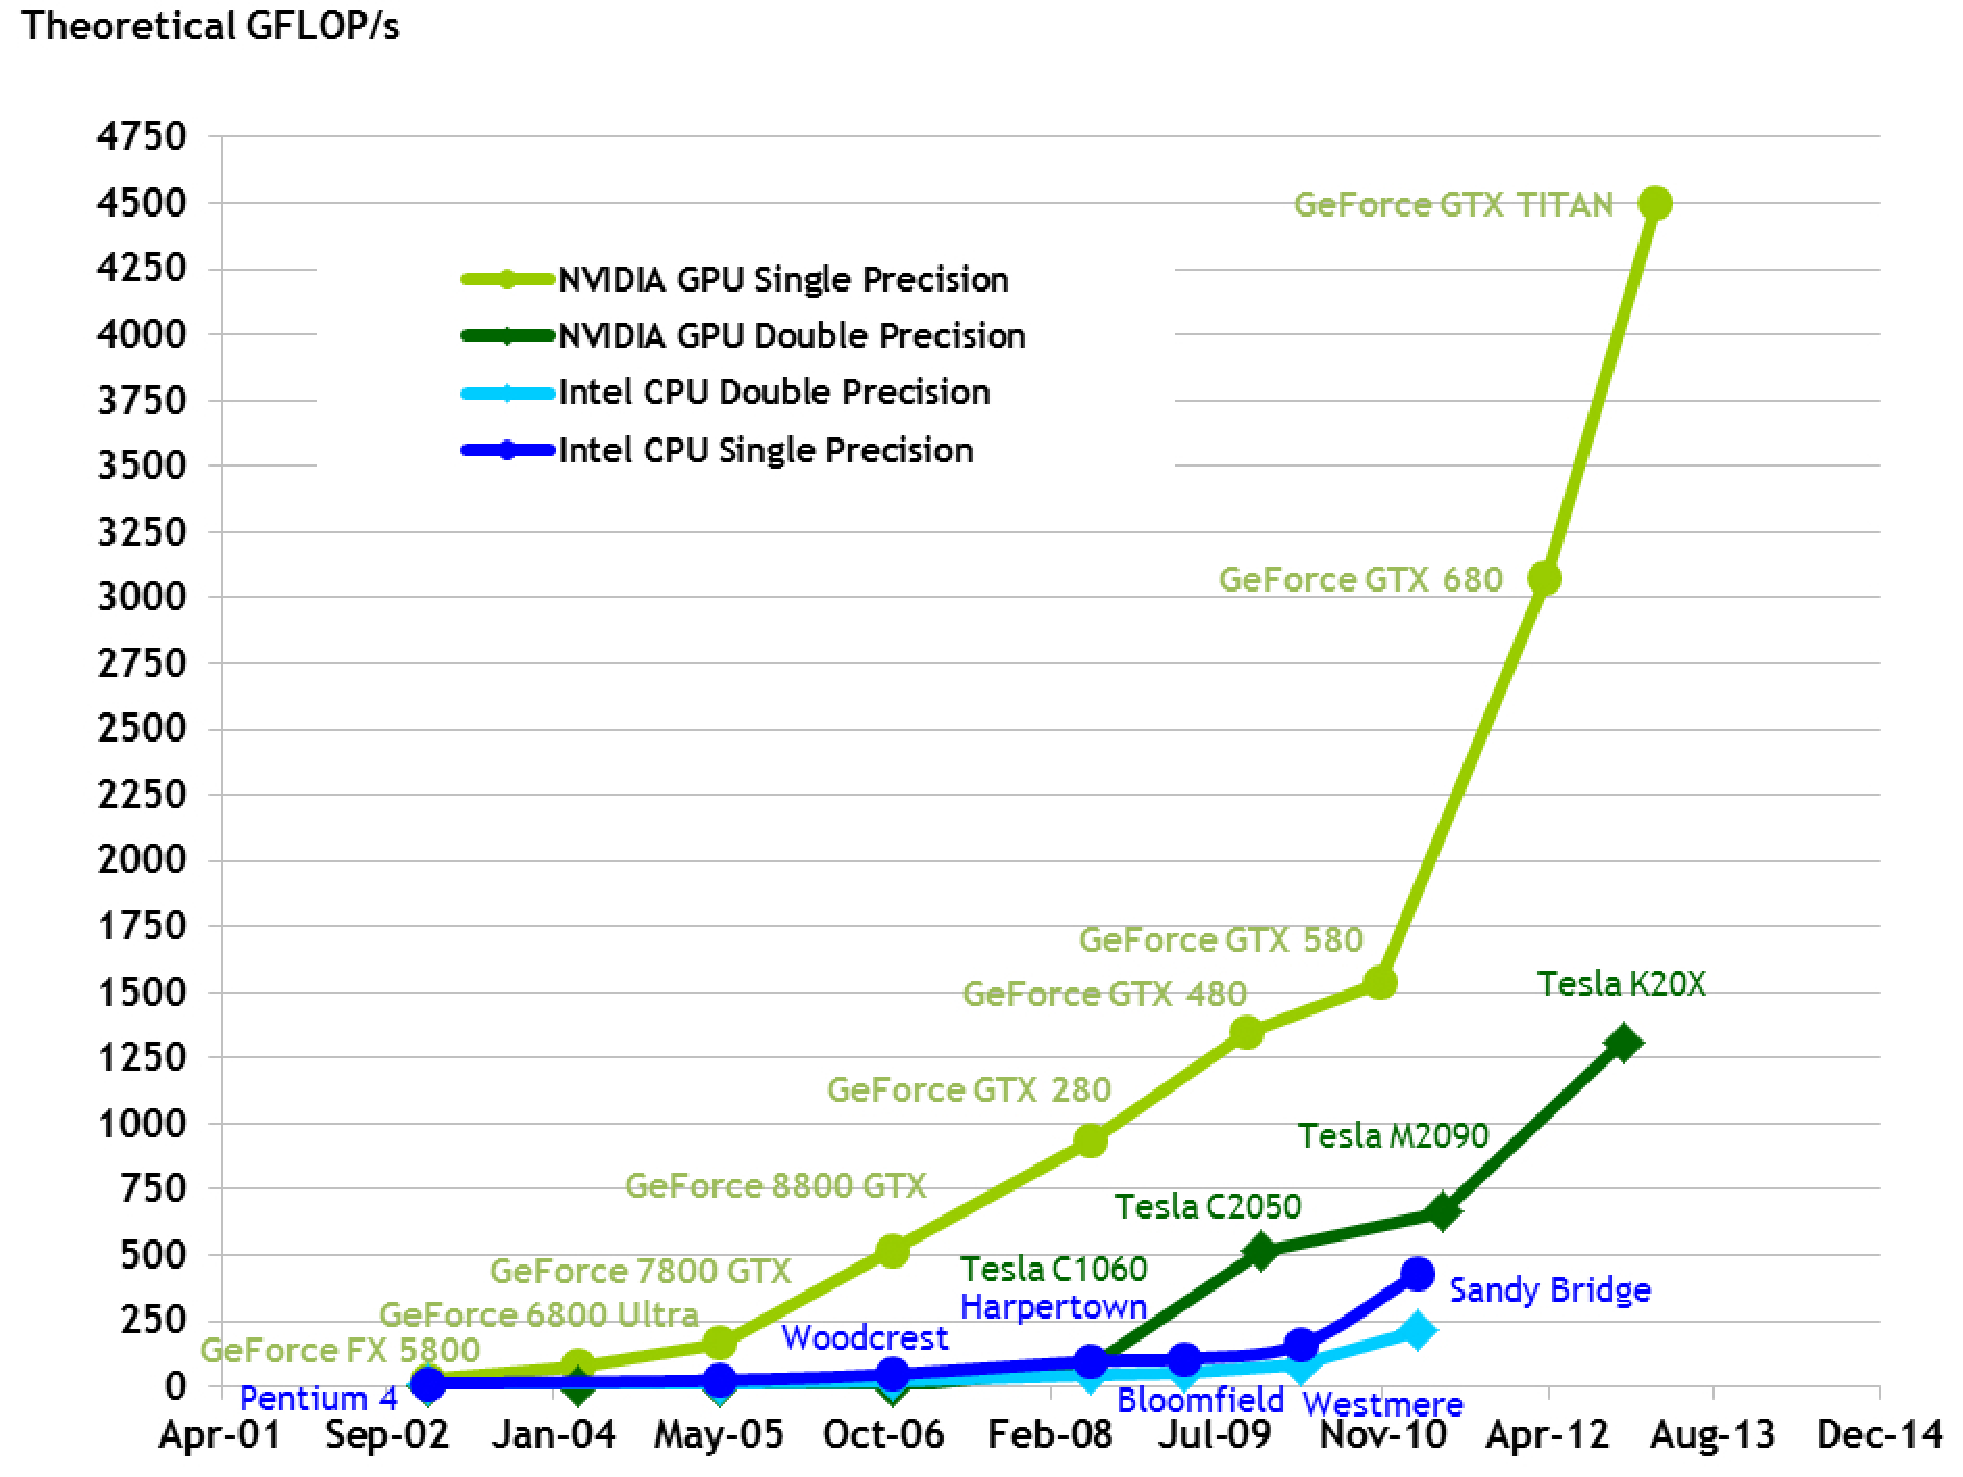
\includegraphics[width=0.6\textwidth]{graphics/computational_cap.pdf}
     \caption[The maximum theoretical GigaFLOPs of various NVIDIA GPUs vs. flagship Intel processors.]{The maximum theoretical GigaFLOPs of various NVIDIA GPUs vs. flagship Intel processors \cite{cuda}. \label{computational_cap}}
\end{figure}

To break into the supercomputing market, manufacturers crated the first programmable, general purpose GPU, which focused on power efficiency and parallelism.  As figure \ref{computational_cap} shows, the maximum theoretical computational capacity of NVIDA GPUs has been increasing faster than that of CPUs \cite{cuda}.  The single-precision performance is much better than the double-precision, however.  The traditional role of GPUs as graphics accelerators did not require double precision capabilities, which is why single precision performance was emphasized during their development.  In recent years, double precision arithmetic is supported as well,
but gaming cards in the GeForce series have much poorer performance than the high-end Tesla cards.  The Tesla cards have substantially more double precision units than the GeForce cards, which is why GeForce double precision is not shown \cite{fermi}.  As Figure \ref{computational_cap} also shows, CPUs have nearly equivalent single and double precision performance. 

The GPU executes differently than a CPU and is a separate piece of hardware.  To use GPUs for real computing, there needed to be an interface between the GPU and CPU and an easy way to program them, so CUDA was created.  CUDA stands for ``Compute Unified Device Architecture,'' and is NVIDIA's parallel computing platform \cite{cuda}.  The next subsections will talk about the details of GPU execution and how CUDA allows them to be programmed. 

\subsection{Architecture}

An NVIDIA GPU's basic processing unit is called a multiprocessor.  These multiprocessors house many individual computational cores and can process jobs independently.  Figure \ref{fermi_SM} shows the architecture of a Fermi-family NVIDIA GPU.  They are often called ``streaming multiprocessors,'' or SMs, as well.

\begin{figure}[h!] 
  \centering
    \includegraphics[width=0.3\textwidth]{graphics/fermi_SM.eps}
     \caption[The architecture of a Fermi multiprocessor.]{The architecture of a Fermi multiprocessor \cite{cuda}. \label{fermi_SM}}
\end{figure}


\begin{figure}[h!] 
  \centering
    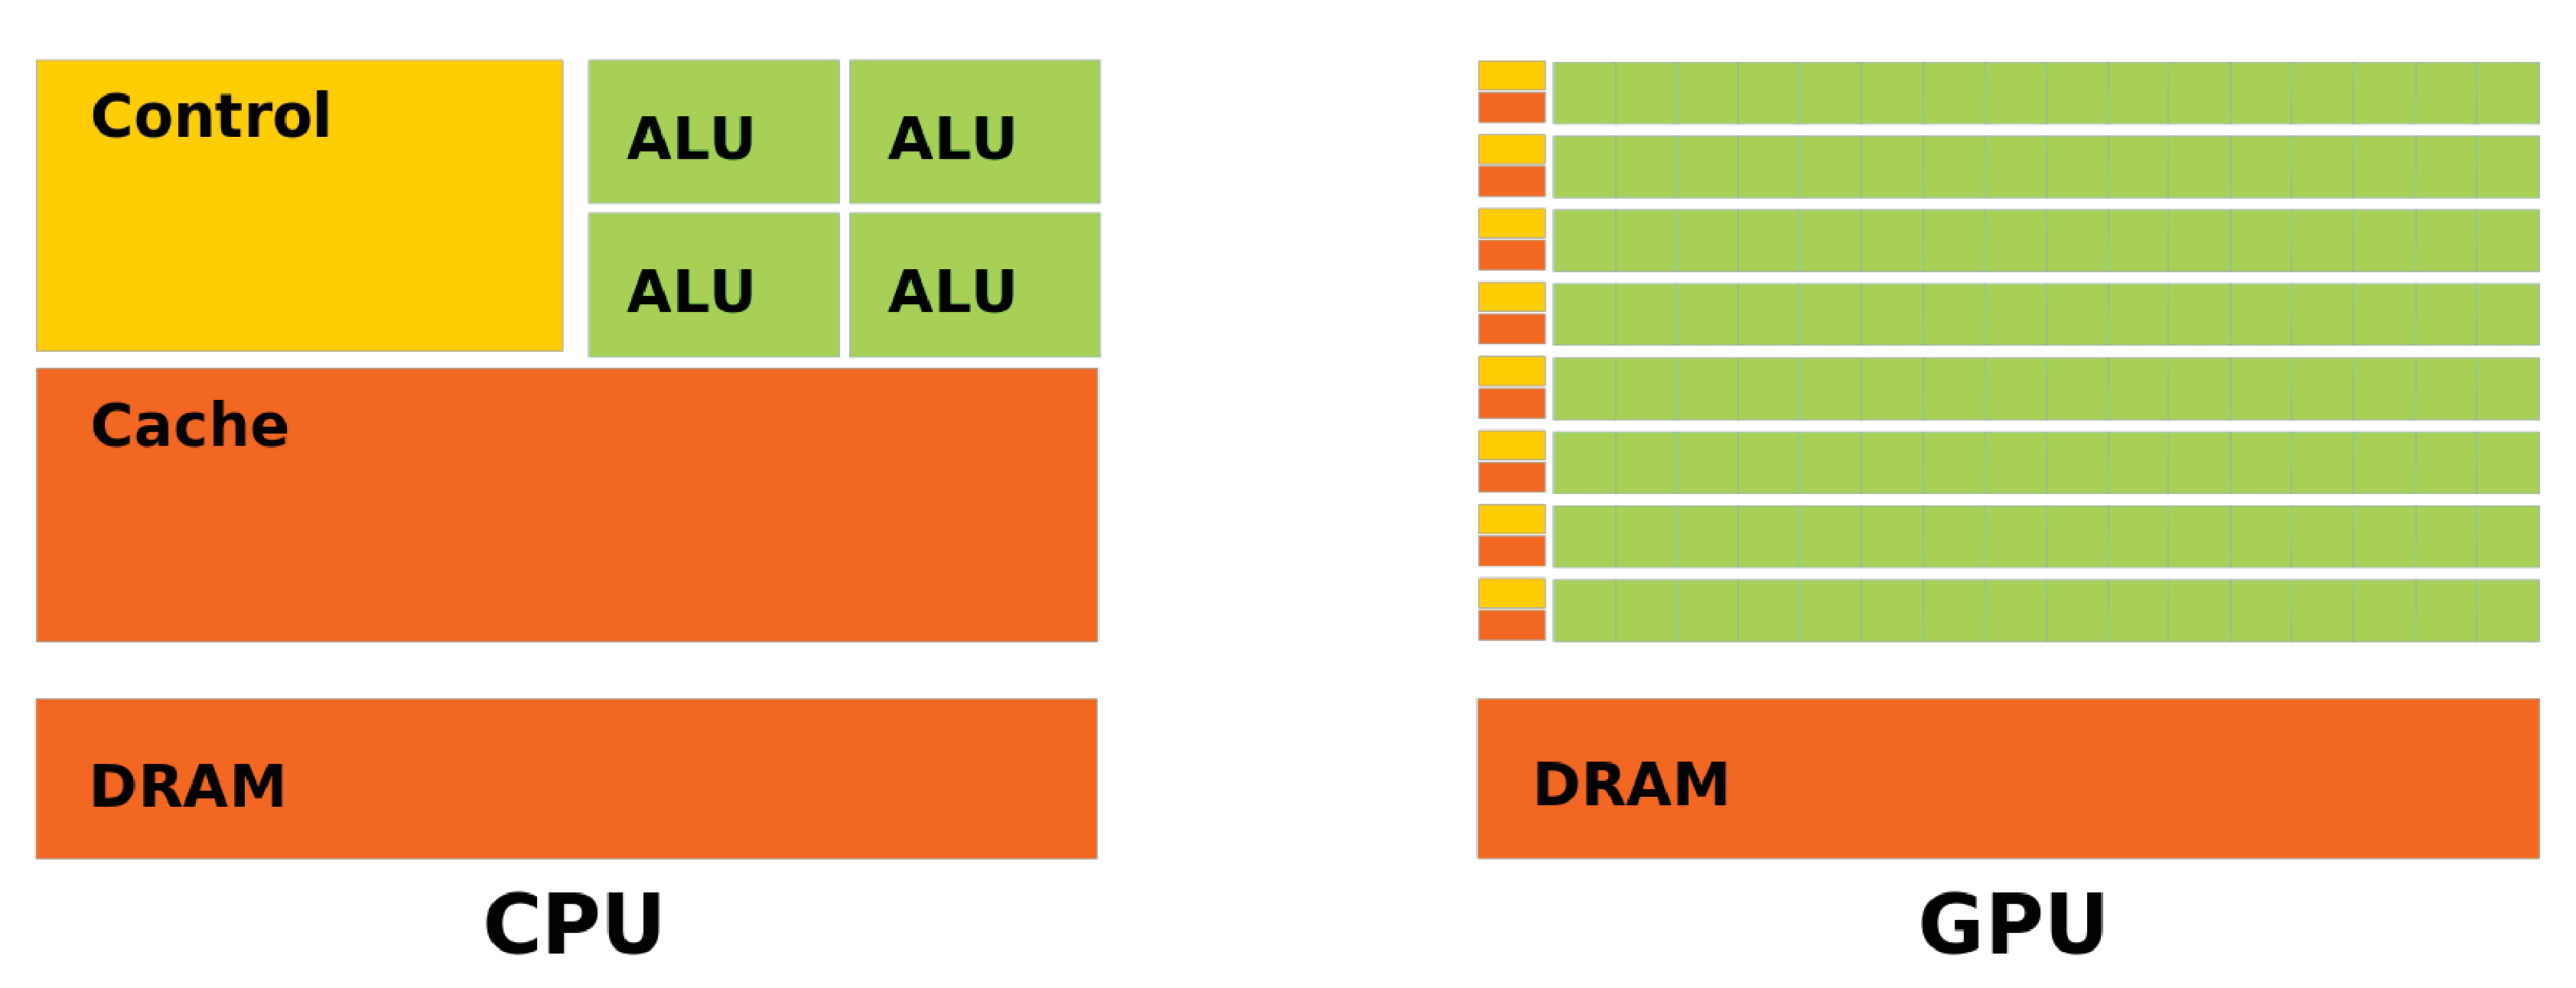
\includegraphics[width=0.8\textwidth]{graphics/CUDA_transistors.eps}
     \caption[Relative transistor space use in GPUs and CPUs.]{Relative transistor space use in GPUs and CPUs \cite{cuda}. \label{cuda_transistors}}
\end{figure}

Part of the reason GPUs are able to perform efficiently is because they rely on single instruction, multiple data (SIMD) execution.  This execution method uses the same instructions simultaneously carried out over multiple pieces of data.  This reduces the amount of power used in control and therefore more math can be done per Watt, which is the main reason why they are being used in supercomputers \cite{exascale}.  There are some tradeoffs for this power efficiency, however, such as requiring relatively simple tasks because of limited cache and control space and requiring data parallelism for full utilization.  

The GPU programming model abstracts SIMD execution by using threads, which can be thought of in the traditional sense. Single-instruction multiple-thread (SIMT) and SIMD are similar in the sense that identical instructions are carried out across different pieces of data, but SIMT allows threads to act independently, albeit with a performance penalty.   When a thread in a multiprocessor executes different instruction than the other resident threads, the multiprocessor masks it from execution, executes the identically-executing threads, then masks the identically-executing threads and executes the \emph{divergent} thread.  This effectively serializes operations if they require different instructions.  This masking and serializing makes many empty spaces in the SIMD lanes of the multiprocessor, and thus can cause severe performance penalties.  The magnitude of the penalty depends on the rate at which data is being delivered to the multiprocessor since work can only be done if data is present.  If the multiprocessor can completes all jobs, even if it needs some serialization, before the next set of data arrives, then the penalty will be invisible \cite{cuda}.

Another benefit of using SIMD is that less transistor space is needed for control and storing instructions, and more transistors can be used for arithmetic.  This is evident in the amount of transistor space allocated to each kind functional unit in a CPU and a GPU.  Figure \ref{cuda_transistors} shows a cartoon of the space allocated to cache, control, and arithmetic units on the CPU and GPU \cite{cuda}.  The CPU has more cache and control space since it needs to be able to execute complicated instructions quickly and to quickly switch between many thread contexts.  The GPU has more arithmetic units since it is geared for computational throughput on data-parallel tasks where less complicated instructions are needed \cite{cuda}.

\subsection{CUDA}

CUDA was first released in 2006 as NVIDIA's proprietary GPU programming platform.  It makes minimal additions to C/C++, and any C programmer would be very comfortable programming in CUDA \cite{cuda}.  It was chosen over OpenCL, the open source GPU programming platform, due to CUDA's greater feature support, stability, ease of programming, wider community usage, and ability to use new, cutting-edge features in NVIDIA GPUs that OpenCL is not.

The overarching theme for CUDA is that a host CPU thread directs the GPU's operation.  Data must be transferred from the host to the GPU's global memory over the PCIe bus, \emph{kernels} are launched to perform computations based on the transferred data, then control returns to the host thread.  ``Kernels'' are CUDA's parallel programs that each thread carries out over the data.  Kernels must specify independent tasks for each GPU thread in the sense that thread execution order does not matter.  There can be barriers where threads will wait for all other threads to arrive, but the order in which the threads execute to get to such a barrier is arbitrary and done by the GPU hardware \cite{cuda}.  Blocks of threads have the same interleaving requirement.  The order in which they execute is unspecified, and cannot be relied on for calculating values.% the same as what? they must be independent?  Makes more sense I hope!
  Blocks of threads are executed simultaneously on a multiprocessor.  The group of all blocks is called a ``grid.''  The grid is analogous to the entire GPU device, blocks are analogous to the multiprocessors, and threads are analogous to the individual cores. Figure \ref{cuda_grid_launch} shows the host-device execution and the organization of threads into blocks and blocks into the grid \cite{cuda}.

\begin{figure}[h!] 
  \centering
    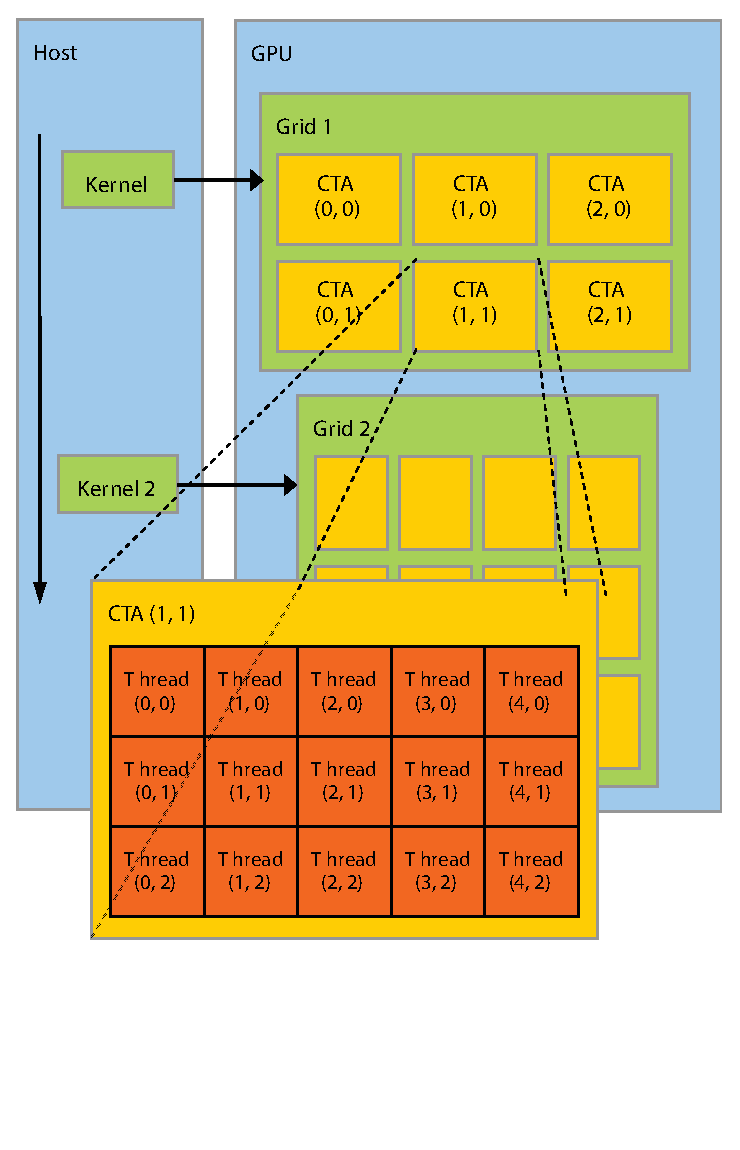
\includegraphics[width=0.4\textwidth,trim= 0cm 2.5cm 0cm 0cm]{graphics/CUDA_grid_launch.eps}
     \caption[Host-device execution in CUDA and the organization of threads into blocks and blocks into the grid.]{ Host-device execution in CUDA and the organization of threads into blocks and blocks into the grid \cite{cuda_ptx_isa}. \label{cuda_grid_launch}}
\end{figure}

Grid and block dimensions can be 1D, 2D, or 3D arrays, which simply influences how the data is indexed.  Every thread has unique variables, ``threadIdx'' and ``blockIdx,'' that are automatically generated upon kernel launch.  The grid dimensions (the number of blocks in each grid dimension) and the block dimensions (the number of threads in each block dimension) are also broadcast to every thread.  Based on these quantities, a unique thread identification number can be computer and used to access the data.   For example, if the grid is 2x2 and blocks are 4x4, a unique thread coordinate can be computed by doing id$_y$ = blockIdx.y * blockDim.y + threadIdx.y and id$_x$ = blockIdx.x * blockDim.x + threadIdx.x.  If the grid and blocks are both 1D, indexing is much simpler, e.g.\ id = blockIdx.x*blockDim.x+threadIdx.x \cite{cuda}.

Even though blocks can be made of up to 1024 threads, when they are executed in a multiprocessor they are scheduled in smaller units that are 32 threads wide.  These units are called \emph{warps}.  The multiprocessor executes the threads in a warp concurrently until all the threads in the thread block are complete.  It then fetches another block form the queue and processes it.  Multiple blocks can be resident in the SM if there are enough resources (registers, etc) to accommodate it \cite{cuda}.

Warps are what abstract SIMD execution.  Warps are like the SIMD vector that must be processed using the same interactions carried out over all the data elements of the vector.  This is why every thread in a warp must execute the same instructions or they are split or are serialized \cite{cuda}.  The low level hardware uses SIMD, but CUDA relaxes SIMD requirements since it allows threads to execute different instructions, albeit with a performance cost.
  
% in a multiprocessor as opossoed to a CPU?  Are there more or less threads in other instances? This sort of sounds like a comparison to something else, but I think you just mean that this is how GPUs work...?  This is just how GPUs work.  No talk about CPUs here.
% How does this abstract SIMD execution? Maybe one more sentence to round out this paragraph more clearly...
%  added a few more sentences, hope it is more clear.

\subsection{Memory}

Bandwidth is the rate at which data can be read from or stored into memory by a processor. High bandwidth is needed to get all of the required data to the arithmetic units and to maintain high computational throughput.  Most optimization work done of GPUs involves relieving memory bottlenecks.  The bandwidths of recent Intel CPUs and NVIDIA GPUs are shown in Figure \ref{bandwidth}, and it can be seen that GPU's bandwidth far exceeds the CPU's.  It is important to remember that this is maximum \emph{aggregate} bandwidth, however, not the bandwidth available to each individual multiprocessor \cite{cuda}.   

\begin{figure}[h!] 
  \centering
    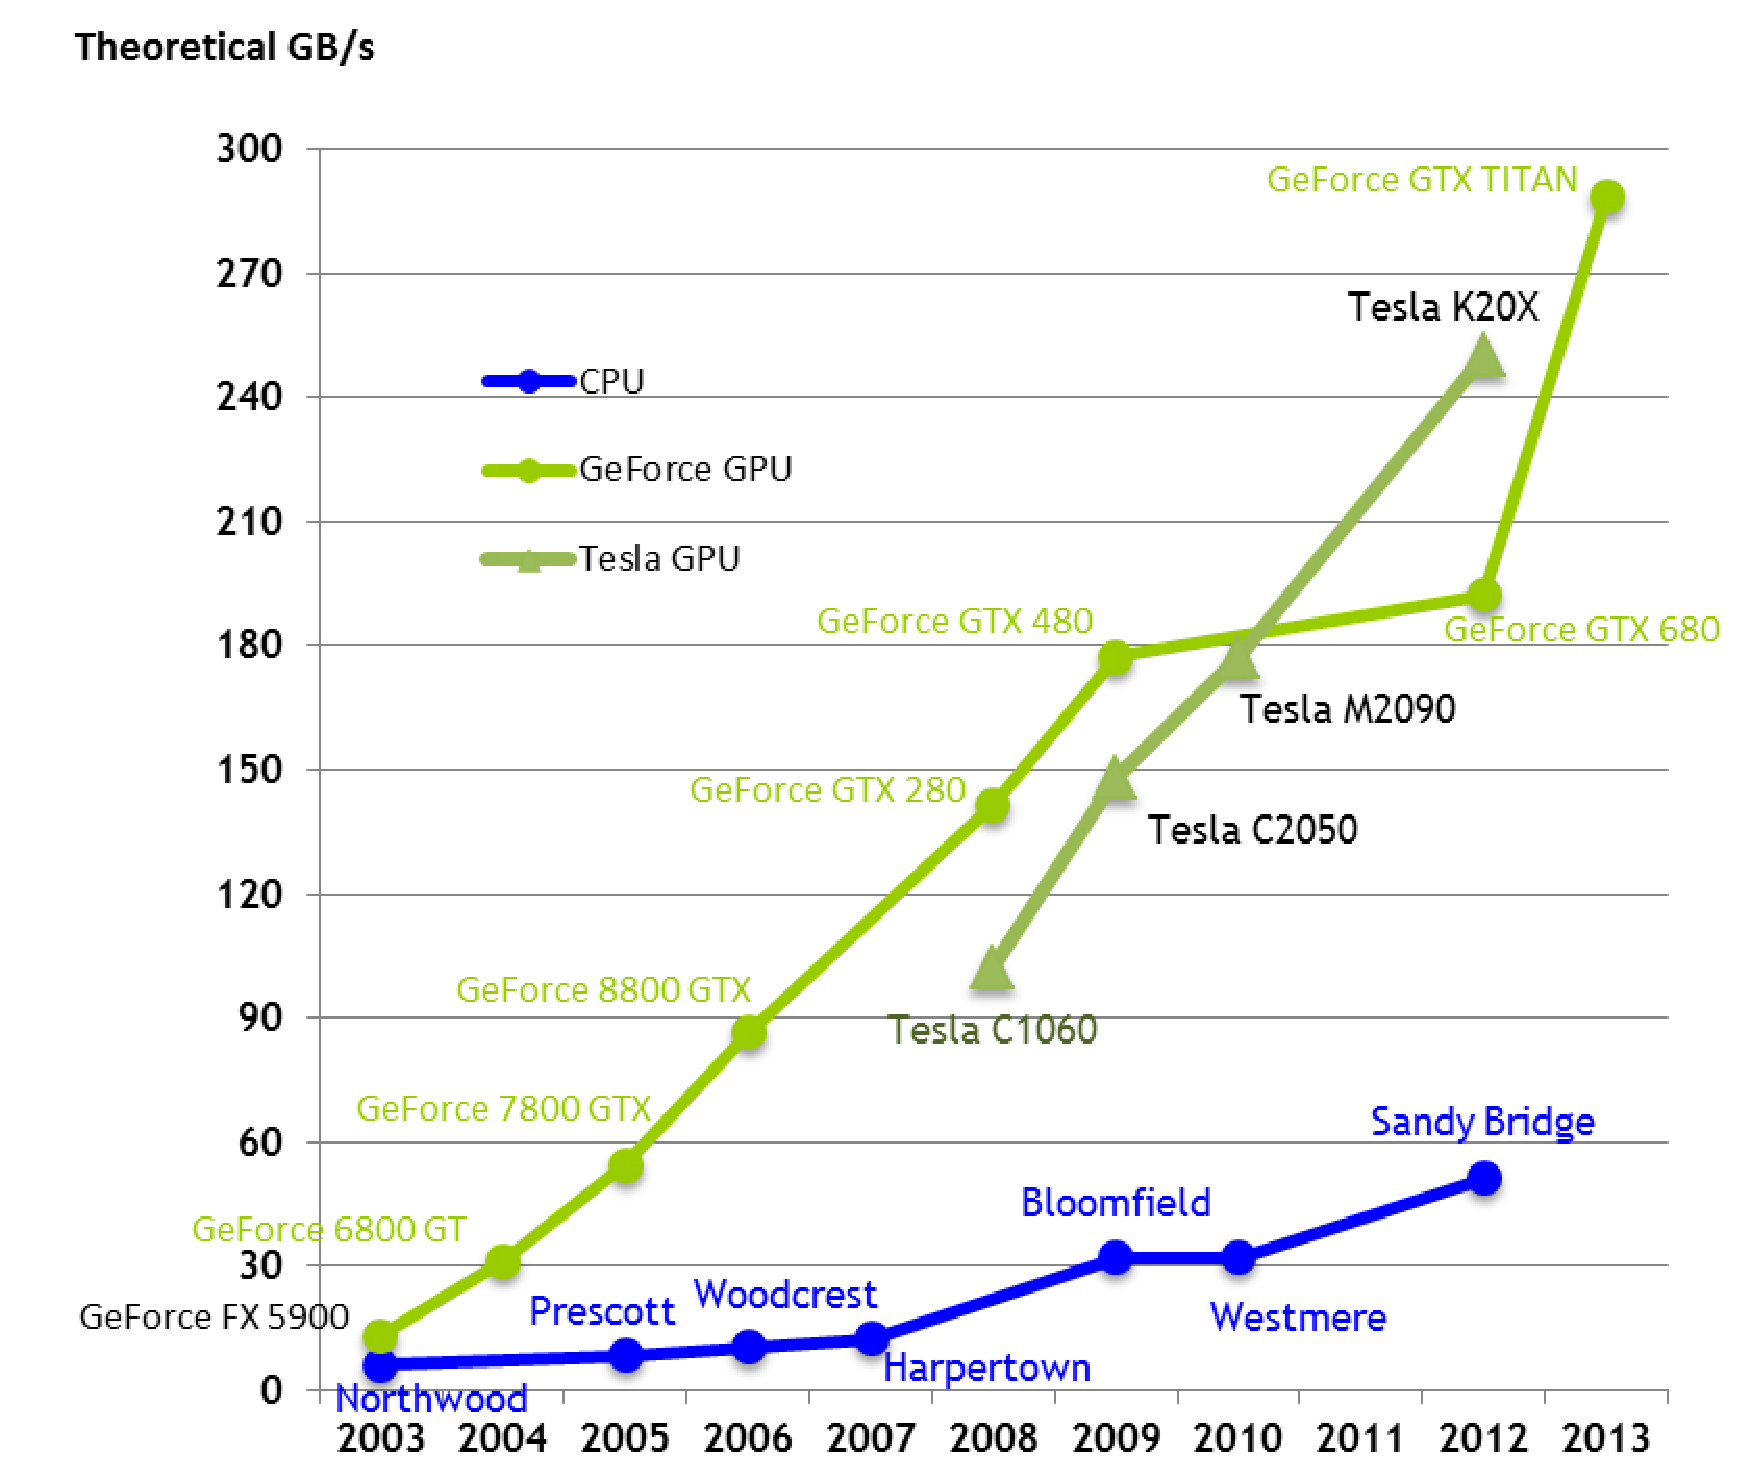
\includegraphics[width=0.6\textwidth]{graphics/memory_bandwidth.pdf}
     \caption[The total global memory bandwidth of NVIDIA GPUs vs.\ flagship Intel processors.]{The total global memory bandwidth of NVIDIA GPUs vs. flagship Intel processors \cite{cuda}. \label{bandwidth}}
\end{figure}

To maximize bandwidth and take advantage of spatial locality in memory, the memory subsystem on a GPU is also SIMD-like, as are most modern CPU subsystems.  When a thread requests a piece of data, not just the piece that is requested is delivered by the subsystem, but rather a chunk of aligned data that contains the requested piece.  If the other loaded values are not used, memory bandwidth is wasted.  For best performance, CUDA requires adjacent threads to access adjacent pieces of data.  This way, memory transactions are ``coalesced.''   In coalesced transactions, every piece of data in the memory payload is used and bandwidth is maximized \cite{cuda}.  Figure \ref{coalesced} shows this graphically \cite{programming_massively}.  If a thread needs to load an entire array, it is better to interleave values in memory so that adjacent memory is accessed at the \emph{same time} by neighboring threads rather than loading adjacent data sequentially by a single thread \cite{cuda}.

\begin{figure}[h!] 
  \centering
    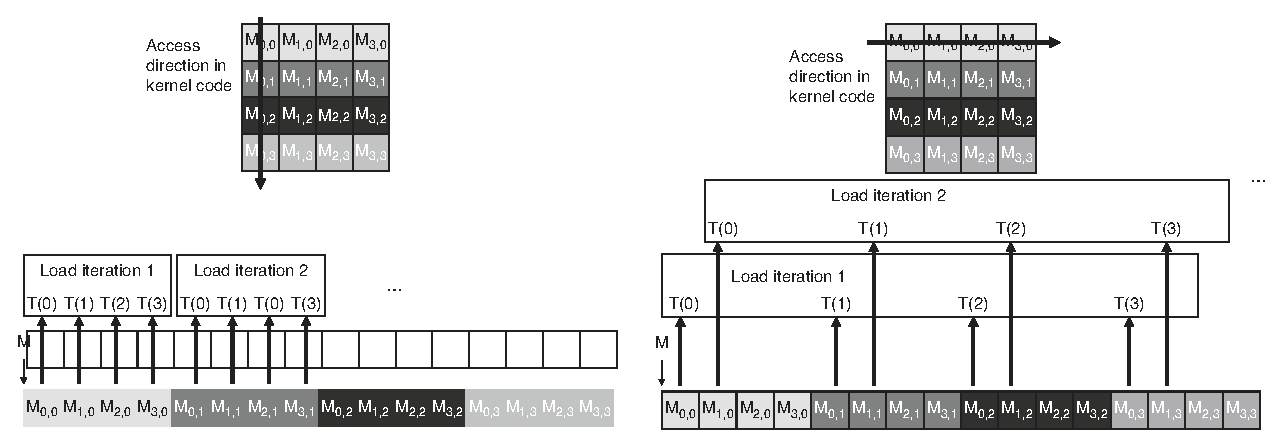
\includegraphics[width=0.8\textwidth]{graphics/coalesced.eps}
     \caption[Memory transactions of CUDA threads.]{Memory transactions of CUDA threads.  Coalesced access on the left and non-coalesced access on the right \cite{programming_massively}. \label{coalesced}}
\end{figure}

GPUs have even higher global memory latency than CPUs, from 200 clock cycles on newer cards up to 800 clock cycles on older cards, compared to about 50 clock cycles on a typical CPU.  CPUs, which are for serial execution, want low latency memory access and do this through multilevel cache structures and large control spaces that allow them to do out of order and speculative execution.  GPUs, which are geared for high throughput, want high bandwidth and hide latency by pipelining many threads.  More transistor space is allocated for computation rather than for trying to minimize memory latency, and instead the memory latency is hidden though parallelism.  Figure \ref{pipeline} shows how GPU threads are pipelined to hide latency whereas CPUs rely on low latency to quickly execute different threads in series \cite{cuda_gtc_pres}.  Thus, GPUs perform best when as many threads as possible are launched \cite{cuda}.

\begin{figure}[h!] 
  \centering
    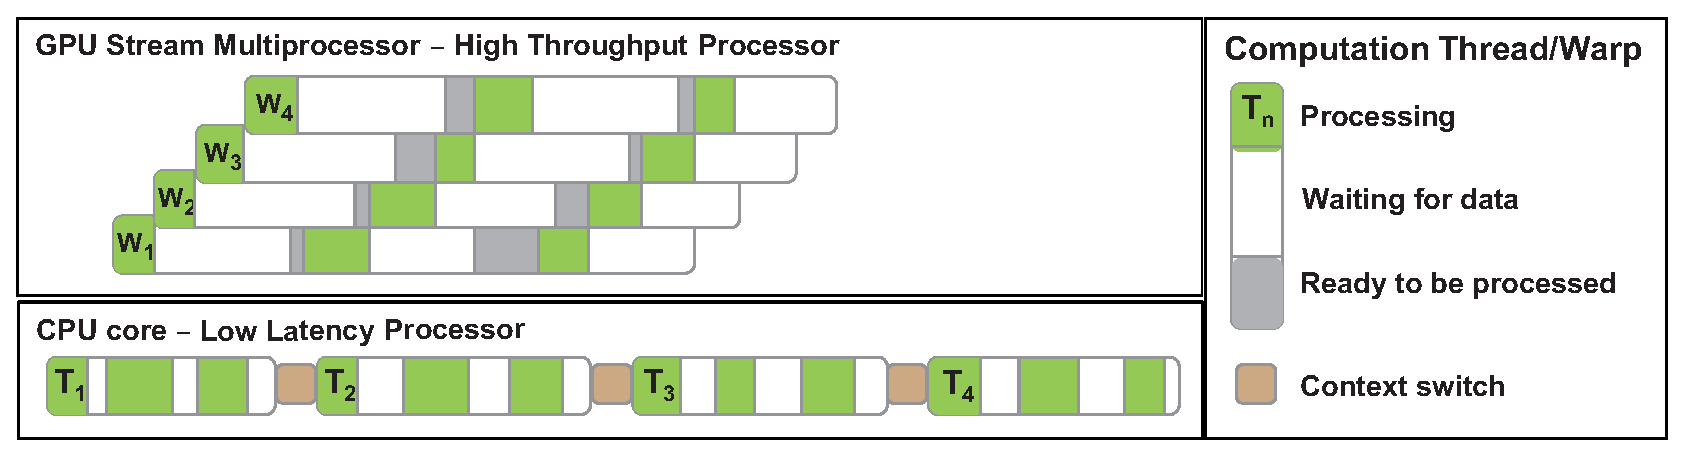
\includegraphics[width=\textwidth]{graphics/pipeline.eps}
     \caption[GPUs Pipeline many threads to hide high memory latency.]{GPUs Pipeline many threads to hide high memory latency \cite{cuda_gtc_pres}. \label{pipeline}}
\end{figure}

Even though there are fewer levels of cache in a GPU than a CPU, there are still many different spaces, each of which has different properties.  Figure \ref{cuda_mem} shows the various memory spaces of an NVIDIA GPU.  The global memory space is the largest memory space and has the greatest latency ($\sim$200 memory clock cycles).  This is the amount of total RAM specified for each card, which can be as small as 512 MB for very low-end cards and up to 12 GB for the largest high-end card.  This memory space is accessible by all threads in all blocks.  

\begin{figure}[h!] 
  \centering
    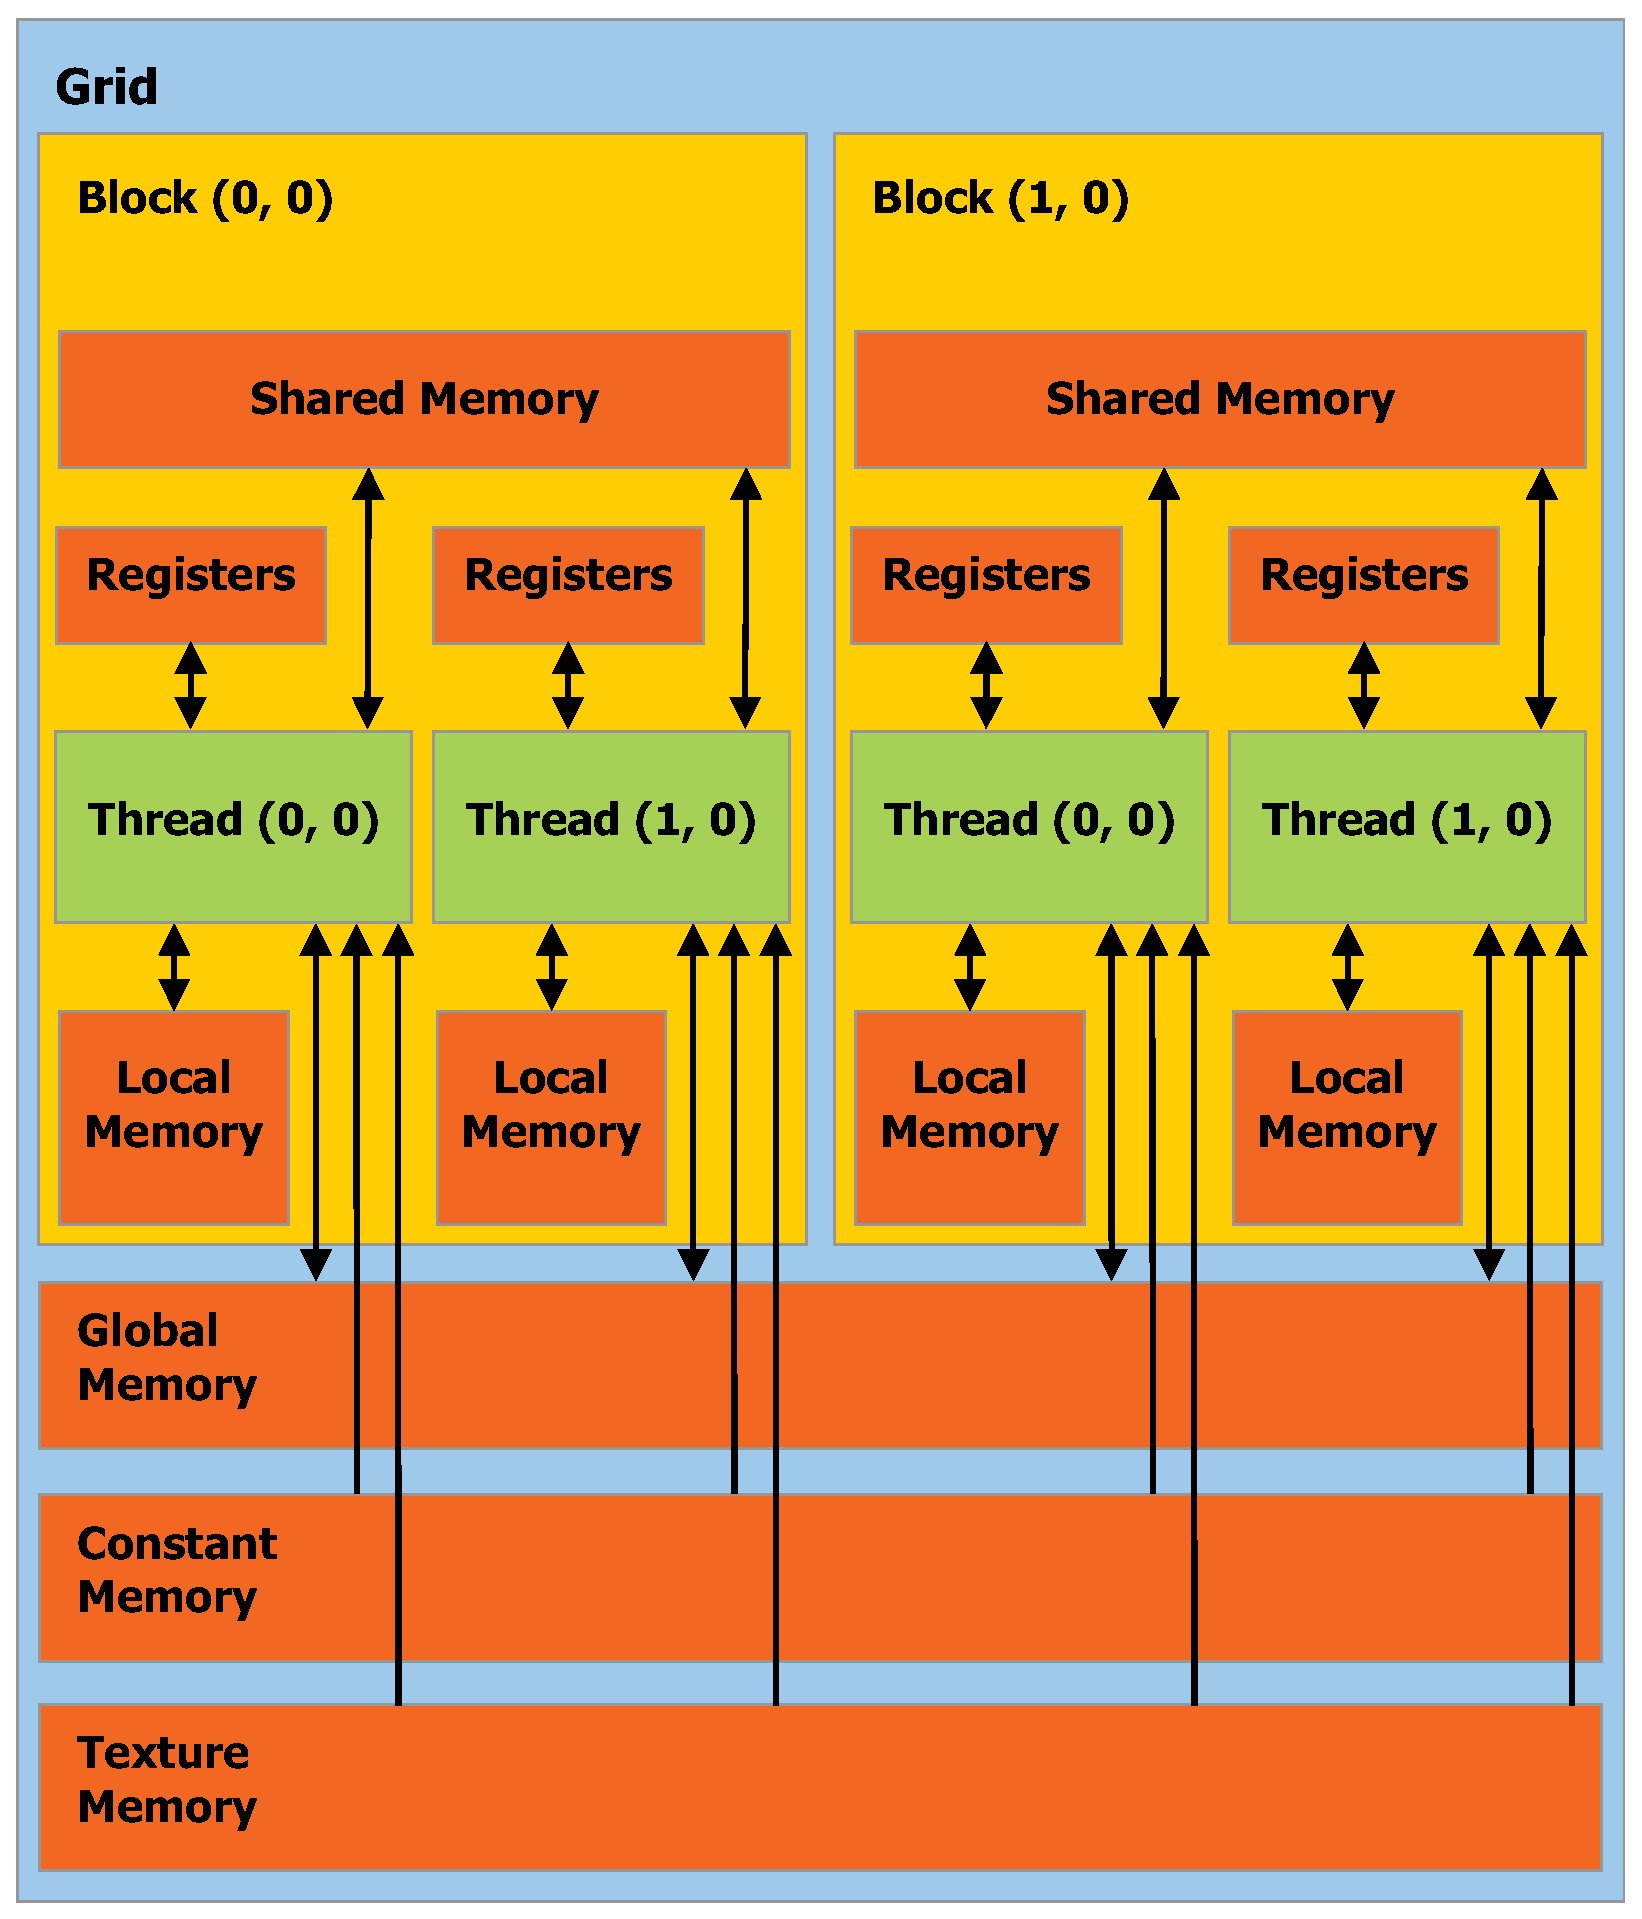
\includegraphics[width=0.4\textwidth]{graphics/CUDA_memory.eps}
     \caption[The memory spaces in CUDA and NVIDIA GPUs.]{The memory spaces in CUDA and NVIDIA GPUs \cite{cuda}. \label{cuda_mem}}
\end{figure} 

The next level down is the shared memory space.  This acts as a user-programmable cache and is not used unless explicitly coded.  It resides on the multiprocessor and has very low latency (on the order of 1 processor clock cycle). The data can be seen by all threads within a block, hence the ``shared'' name.  The shared memory space can allow intra-block communication  without incurring the high penalty of global memory transactions and can therefore improve performance by acting as a cache, storing any data that is reused by threads \cite{cuda}.  

% You might want to quickly define cache, or the distinction between L1 and L2 cache, etc. I know it's annoying - but your audience may not know that much about hardware (and they'll learn so much from your dissertation now!). Also, paging local memory may be unfamiliar to people.  done and done.
The next level down is the local memory, which is thread-specific.  The local memory serves to hold any data that cannot fit into the registers.  It is not truly ``local'' since it is actually stored in global memory, but in Fermi and newer architectures the local memory is cached by an L1 cache on the multiprocessor.  A cache is a small, but very fast, storage area for data between the processor registers and global memory.  Caches hold data that has been loaded into the processor previously.  If the data is required again, it can be loaded from the cache instead of the global memory.  Loading from cache is much faster than loading form global memory, and caching increases performance by taking advantage of data reuse.  There are multiple levels of cache as well, each of which are numbered.  Lower numbers (e.g. L1) are faster and closer to the registers, and larger numbers (e.g. L2/L3) are typically slower and larger.

Registers, the lowest level of memory, are what the arithmetic units directly load their data from.  They are fast, but have a limited size, which is why local memory is used to page them.  Paging means that any data that does not fit into the registers is stored in the local memory.  When the processor requests a value that has been paged, it is fetched from local memory and swapped for a register value.   A Fermi GPU has a large register file (2 MB) compared to a typical CPU ($\sim$6 kB) % as compared to what?  to a CPU
, but each multiprocessor only has 128 kB and that is further subdivided by each thread (maximum register size per thread is 63 kB) \cite{fermi}.

The other memory spaces are the constant memory and the texture memory, which are both visible to all threads in all blocks.  They aren't truly separate spaces, but rather global memory that is handled differently.  Storing data in the constant space means that it cannot be written over (hence the ``constant'' name), but the data is cached so data reuse by threads can result in a cache hit and the global memory itself does not need to be queried \cite{cuda}.  Constant memory is limited to 64kB, however, and is cached by 8kB caches on each multiprocessor, so large datasets cannot be stored in constant memory.  It also performs best when values are broadcast to all threads.  Texture memory is also cached, but its cache is optimized for 2D spatial locality in the texture coordinate system instead of actual memory locality, and it does not have a maximum size.  Another feature of the texture memory is that is can perform low precision linear interpolation in the same transaction as a read \cite{cuda}.

\section{OptiX}

To save time and effort, NVIDIA's OptiX ray tracing framework is used by WARP for the geometry representation, surface detection, and material queries on the GPU.  The programmer must write all geometric intersection programs for the geometry primitives as well as the geometry hit programs.  OptiX provides the mathematical and computer science glue between the user-programmed ray tracing elements.  Besides its flexibility, OptiX provides optimizations that would require many months for a single developer to replicate in handwritten code.  It's main optimization is automatically producing high-quality acceleration structures for traversing the primitives in the geometry \cite{optix}.  In this section, the general properties and workings of OptiX will be presented.  Details about its implementation in WARP will be discussed in Chapter \ref{chap:imp}.

\subsection{OptiX Programs}

As stated before, the developer must provide all the programs for OptiX.  These various programs are compiled to .ptx files, the paths to which are given to the OptiX API at compile time and are loaded by the executable at run time \cite{optix}.  The programs are compiled to .ptx because it is a ``virtual assembly language'' that can be easily interpreted by GPU and requires no further compilation.  Figure \ref{optix_flow} shows the control flow in OptiX.  The launch is just like a CUDA kernel launch.  The API checks to make sure all the necessary data is present on the card, then launches kernels internally to carry out the trace on the GPU.

\begin{figure}[h!] 
  \centering
    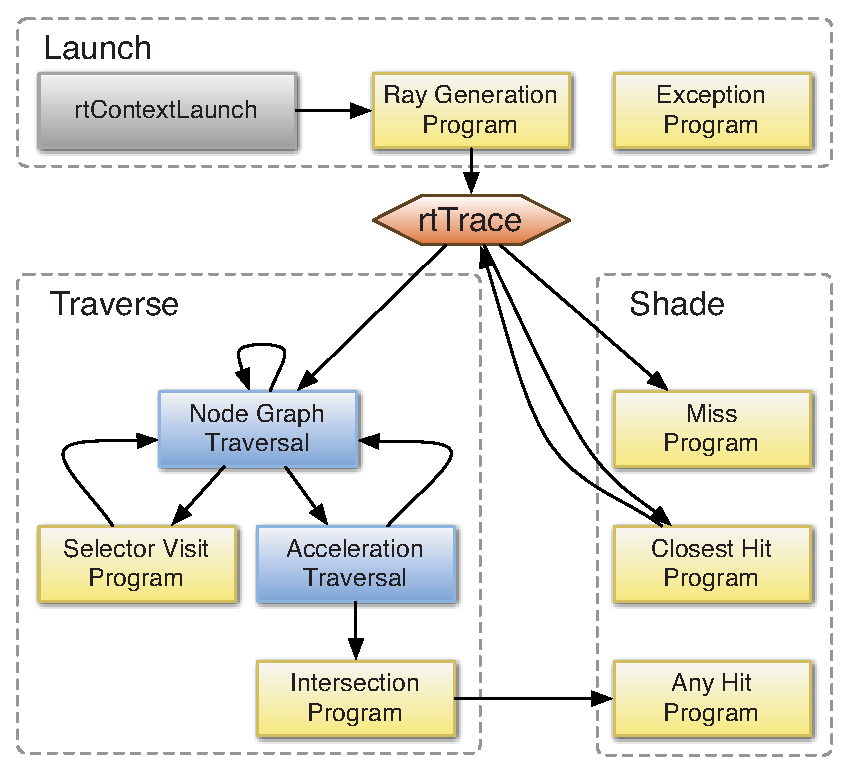
\includegraphics[width=0.5\textwidth]{graphics/optix_flow.eps}
     \caption[The program flow in a launched OptiX context.]{The program flow in a launched OptiX context \cite{optix_paper}. \label{optix_flow}}
\end{figure}

The ``ray generation'' program is like a ``main" function in the ray tracer. It initializes rays, their starting points and directions, and specifies the data that they report.  Once this is done, the trace is executed. The trace traverses the geometry and find intersection points.  If \emph{any} geometry primitive is intersected, the ``any hit'' program is executed.  In graphics rendering problems this program is typically used for determining areas that are completely occluded from the light source, therefore terminating the trace. I have not though of a good use for shadow rays, but they could potentially be used for an adjoint-type of calculation or variance reduction schemes to terminate neutrons according to some criteria.  %translation to NE?  Dunno really...
  As OptiX queries the primitives along a ray, it tightens an interval on $t$, the path length of the parameterized ray \cite{optix}.  The equation for a parameterized ray is shown in \eqref{parameterized_ray}, where $\vec{r}_P$ is the end point of the ray, $\vec{r}_O$ is the origin point of the ray, and $\vec{r}_D$ is the directional unit vector of the ray.  Figure \ref{ray_surface} shows an illustration of a ray-surface intersection.

\begin{equation}
\label{parameterized_ray}
\begin{split}
\vec{r}_P = \vec{r}_O + t \vec{r}_D 
\end{split}
\end{equation}

\begin{figure}[h!] 
  \centering
    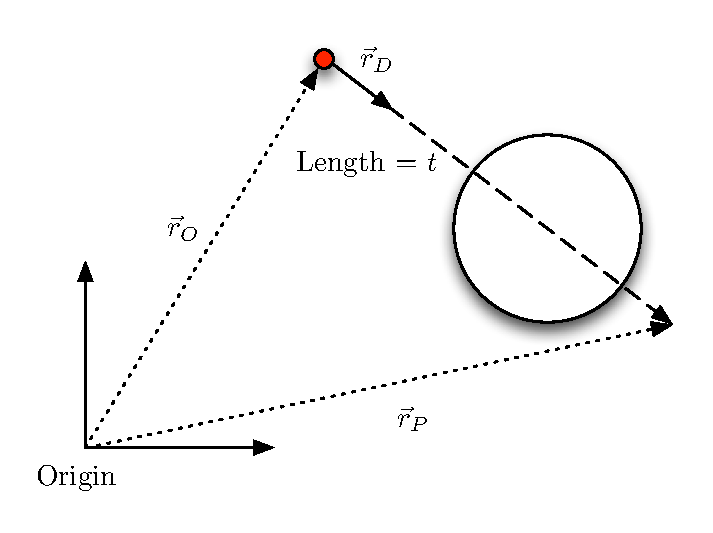
\includegraphics[width=0.5\textwidth]{graphics/ray_surface.eps}
     \caption{Ray-surface intersection: a sphere and a parameterized ray. \label{ray_surface}}
\end{figure}

When the $t$ interval becomes tight enough to determine the closest hit, the ``closest hit'' program is executed.  This program typically returns the closest intersection point to the ray generation program, which then uses this information to shade a pixel in an image, or in WARP's case, determines if a neutron travels past a surface.  Miss programs tell a ray what to do if it does not intersect any primitives \cite{optix}.  In rendering, this usually maps to a scene background image.  Since a material must always be defined in WARP, a miss simply throws an error. This is analogous to a lost particle in traditional Monte Carlo codes.

\subsection{Geometry and Intersection Programs}

Geometrical primitives in OptiX are represented by their intersection programs.  Intersection programs have two purposes - to calculate the exact intersection points between a ray and a primitive and to provide axis-aligned bounding boxes around the primitives.  These bounding boxes must completely contain the underlying primitive, but should be as small as possible for best performance.  Bounding boxes are queried when the acceleration structure is built over the geometry, which is discussed in the next subsection \cite{optix}.  

The main purpose of an intersection program is to calculate the intersection points, which must be reported back in terms of the $t$ value.  For example, the equation for a sphere is $r^2=x^2+y^2+z^2$.  Substituting \eqref{parameterized_ray} into this equation and solving for $t$ yields \eqref{ray_sphere}.  Since a sphere is a closed surface, there are two intersection points.  The smallest nonnegative value is reported back by the intersection program.

\begin{equation}
\label{ray_sphere}
\begin{split}
a &= \vec{r}_D \cdot \vec{r}_D = 1\\
b &= 2 \vec{r}_O \cdot \vec{r}_D = 2b_2\\
c &= \vec{r}_O \cdot \vec{r}_O - r^2 \\
t &= \frac{-b \pm \sqrt{b^2-4ac}}{2a} = -b_2 \pm \sqrt{b_2^2-c}
\end{split}
\end{equation}

 \begin{figure}[h!] 
  \centering
    \includegraphics[width=0.8\textwidth]{graphics/node_graph.eps}
     \caption[Node graph used for geometry representation in OptiX.]{Node graph used for geometry representation in OptiX \cite{optix}. \label{node_graph}}
\end{figure}

The framework by which geometric primitives are arranged into a scene is very flexible in OptiX.  Figure \ref{node_graph} shows the node graph representation of the geometry that a ray traverses in OptiX \cite{optix}.   The node types and connections are completely specified by the user.  Rays enter the graph at the root node, or ``entry point,'' and it must be specified before a trace can begin \cite{optix}.  From the root node, rays start to query the geometry nodes in the rest of the graph.  Intersection program are run when a ray visits a geometry node to determine the $t$ values of the geometry contained in the node.  Some nodes only serve to contain other nodes, like a ``group'' node.  A group can have children of any kind, whereas a ``geometry group'' can only have ``geometry instance'' children.  
A ``geometry instance'' is a object that combines a geometry primitive, which describes the geometrical object, and a ``material.''  
A material is another name for the closest and any hit programs, and serves to package them into an object that they can be attached to multiple geometry primitives.%?  hopefully clearer now
OptiX can handle different ray types, typically one for radiance and one for shadow, and a geometry primitives can be attached to multiple materials to handle these ray types in different ways.  WARP only uses radiance rays, and using shadow rays was not considered during its development.  
The way in which they traverse the graph depends on the acceleration structures attached to the nodes.  These structures allow the rays to only query objects along their line instead of having to query all objects.  How the geometry nodes are arranged in the graph greatly affects trace performance, as will be seen in Section \ref{sec:prelim}.
  % okay - this paragraph could use some clarifying... hopefully clearer! :/

There are two special node types that can have geometry group children - a selector node and a transform node.  A selector node will decide which geometry group to send a ray down based on some type of criterion.  This criterion can be based on a  global variable that is assigned before a trace or a piece of data that is determined during the trace itself.  It gives the framework more flexibility for the types of problems it can handle and the ease at which solutions can be implemented.  

A transform node transforms the underlying geometry based on an affine transformation matrix.  This node type can be useful for specifying one geometry instance node that is then instanced throughout the scene with different transform nodes.  A transform node can also be used to move geometry based on time.  For WARP's purposes this functionality could potentially be used for calculating the effects of geometric perturbations or even introducing time-dependent simulations.  When transform nodes are specified, they must be attached to a geometry group and be given an affine transformation matrix.  In three dimensions, this is a 4x4 matrix that can specify rotation, scale, translation, and shear.  An example matrix for simultaneous translation and rotation is shown in \eqref{affine} where $dx$, $dy$, and $dz$ are translations in $x$, $y$, and $z$, respectively; and $\theta$ is a rotation around the $z$ axis, i.e.\ a rotation in the $x$-$y$ plane \cite{affine}.  

\begin{equation}
\label{affine}
\vec{x} = \left[ \begin{array}{c}
x \\
y\\
z\\
1 \\ \end{array} 
 \right] \qquad
M = \left[ \begin{array}{cccc}
\cos \theta & -\sin \theta & 0 & dx \\
\sin \theta & \cos \theta & 0 &  dy\\
0 & 0 & 1 & dz\\
0 & 0 & 0 & 0\\
\end{array} \right]  \qquad
M \vec{x} = \vec{x}^\prime
\end{equation}

The final, and arguably most important, part of the node graph is the acceleration object.  This node specifies the acceleration data structure that is attached to each group or geometry group and \emph{must} be present for rays to traverse these groups.  Groups and geometry groups can share acceleration objects, but if any underlying geometry is changed, the structure must be rebuilt for both groups sharing the acceleration object.  Simpler acceleration object layouts typically have better performance, however, since the acceleration objects higher up in the graph can only treat groups further down \cite{optix}.

\subsection{Acceleration Structures}

The basic idea behind acceleration structures is that they provide a way to decompose the scene geometry into a hierarchical graph.  Once this is done, parts of the scene that rays aren't close to intersecting can be pruned from the set of actual geometry primitives a ray must query to find intersection points \cite{optix}.  OptiX provides different types of acceleration structures, namely, bounding volume hierarchy (BVH) trees and k-dimensional (k-d) trees.

BVH is object-centric in the sense that it places boundaries around groups of objects.  Each leaf of the tree can contain one or more objects. K-d trees are space-centric in the sense that they partition the space objects lie in.  K-d trees are binary trees that partition each volume into two smaller volumes until the lowest leaves only contain a portion of a single object.  Figure \ref{bvh_kd} shows how BVH and k-d trees partition the objects and the space, respectively.  BVH trees have the benefit of being shallower, and therefore fast to traverse, but some objects' higher bounding volumes can overlap, leading to situation where both subtrees must be queried.

\begin{figure}[h!] 
\centering
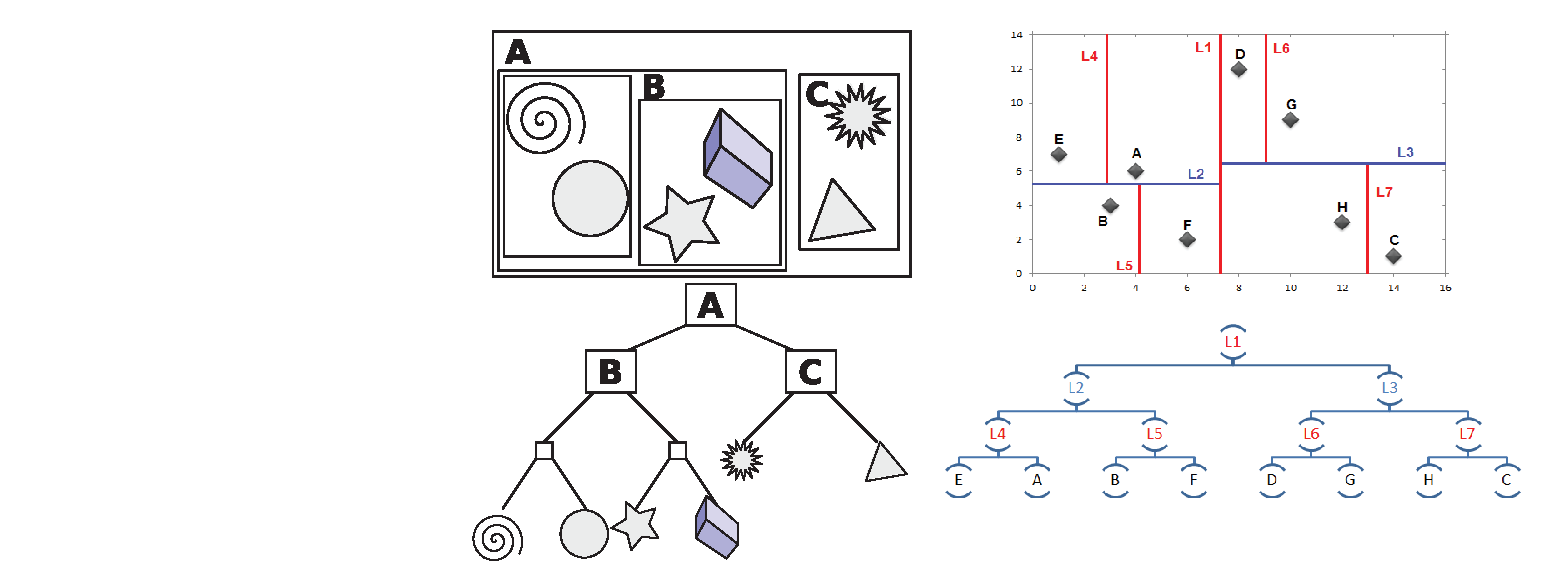
\includegraphics[width=0.8\textwidth, trim= 8cm 0cm 0cm 0cm ]{graphics/bvh_kd.eps}
\caption[Spatial partitioning schemes with the resulting trees.]{Spatial partitioning schemes (top) with the resulting trees (bottom). A BVH tree \cite{wikimedia_bvh} is on the left and a k-d tree is on the right \cite{wikimedia_kd}.   \label{bvh_kd}}
\end{figure}

The benefit of these acceleration structures is that they can be queried in $\log(N)$ time rather than in linear time since major portions of the geometry do not need to be queried or intersected.  OptiX automatically builds these trees over the geometry without any user input other than to specify the type.  The two different types have tradeoffs in terms of size, build speed, and performance. Since WARP's geometry is static and relatively simple compared to photorealistic rendering jobs, the build speed and size have negligible impact%, so the highest performance structure is used in WARP.  % I suspect the photorealistic jobs still choose the best-performing option...
Determining which structure provides the best performance is the goal of one of the preliminary studies in Section \ref{sec:prelim}.  

The typical geometry representation in Monte Carlo neutron transport codes is combinatorial geometry, which uses union and intersection operations on the surface sense  of a point in relation to second-order polynomials.  This kind of algorithm is linear with the number of \emph{surfaces} present in the geometry, so using OptiX in complicated geometries should provide provide a performance boost to geometry routines compared to MCNP or Serpent.  The algorithms in both of these codes do use a form of acceleration, however.  They use a  ``universe'' representation to provide some level of acceleration in determining which material and/or cell a neutron is in.  Universe ``0'' is typically the lowest-level, i.e. the what exists in the problem geometry.  Each cell in universe 0 can either contain a defined material, or it can contain another universe.  If it contains another universe, the neutron coordinates are transformed from the global values to the new universe's.  Once the neutron is in this new universe, only cells contained in it need be considered instead of all the cells in the problem.  Of course, cells in the new universe can contain other universes, and this cell query operation is done recursively until the actual material the neutron is traveling in is determined \cite{jaakko}.  Using ``universes'' in this way is like traversing a k-d tree.  It partitions the geometry based on their spatial relationships and allows a neutron to determine which cell it is in quicker by eliminating far-away cells from the set of cells that need to be queried.  When the runtimes of Serpent, MCNP, and WARP are compared in Chapter \ref{chap:results}, it will be seen how the various geometry representations scale with object number.
 % I don't quite understand what this means?  --- I hope better now....

%%%%%%%%%%%%%%%%%%%%%%%%%%%%%%

\section{Previous Works}

The impetus for developing WARP was the research done by Martin and Brown in 1984 \cite{vector} and by Vuji\'{c} and Martin in 1991 \cite{vujic_vector}.  In the 1984 paper, a method for mapping the Monte Carlo problem onto SIMD vector computers is described.  The essential idea is to bank the neutrons into vectors based on their required operation.  If a neutron is scattering, its data is placed in the scattering buffer.  This operation is called a ``shuffle'' and it actually moves data into contiguous blocks based on the reaction type.  If a neutron needs to do a surface crossing calculation, it is put in the crossing buffer, and so on.  Once a buffer becomes full, it is processed in a SIMD fashion by the vector computer.  

This new approach was named ``event-based'' Monte Carlo, since the neutron events are tracked and processed as a group \cite{vector}.  This was a very different way of performing a Monte Carlo simulation at the time.  Almost all computers were strictly serial, and SIMD lanes were only available in supercomputers.  Therefore, the pervasive method was the ``task-based" method in which neutrons are tracked for their entire lifetime in series.  Since GPUs are massively parallel and rely on SIMD, an event-based algorithm seems to be the appropriate approach to GPU-accelerated neutron transport.  

In the 1991 paper, a vectorized approach is applied to the collision probability method (CPM), which is a deterministic way to solve the integral form of the neutron transport equation \cite{vujic_vector}.  The paper does not directly deal with any type of Monte Carlo simulation, but the addresses the topics of transferring a scalar, CPU-optimized program to a vector computer and discusses why global restructuring of CPU optimized codes is necessary to fully exploit highly vectorized architectures.  This paper served as inspiration to start WARP from scratch instead of trying to completely restructure an establish CPU-based code.
% This sentence feels totally random. Do you use this idea? How does it fit into the picture?  it doesn't, I just wanted to cite jasmina

Vectorizing the Monte Carlo algorithm should allow for GPU execution, but a paper by Zhang \cite{on_the_fly_remapping} also shows that by remapping data references, the thread divergence in GPU warps can be minimized.  This paper provides a simple way to ``vectorize'' the GPU data without actually moving data itself.  This method may lead to sparse data access, but this will happen in a Monte Carlo algorithm anyway so it may be of use to reduce thread divergence and increase the number of active warps per active cycle on the GPU.  Incorporating Zhang's idea means that the algorithm that WARP uses in its event-based transport algorithm differs from the methods in \cite{vector} and\cite{vujic_vector} in that WARP will use a reference remapping vector instead of a shuffle operation.  Data will not actually be moved, rather only the references to the data. 

Although there has been much research done on Monte Carlo neutron transport, there is relatively little research about performing Monte Carlo on GPUs since GPGPUs are a new technology.  There have been two significant developments, however.  One is by Adam Gregory Nelson, who published work on a GPU accelerated Monte Carlo neutron transport code he wrote for his Master's research at Pennsylvania State University \cite{nelson}.  In his thesis, he reports on developing a task-based Monte Carlo Neutron transport code, LADON, and an event-based Monte Carlo Neutron transport code, CERBERUS.  Both codes have CPU versions that have the extension ``c'' and GPU versions that have the extension ``g.''  

Comparing both codes, Nelson was able to attain a 24x speedup between LADONc and LADONg, and a 1.13x speedup between CERBERUSc and CERBERUSg.  These results are very encouraging and show that significant speedups can be realized by performing Monte Carlo neutron transport on the GPU, but discouraging since the event-based speedup was so poor.  Nelson also states that the poor performance of CERBERUS was due to the sorting of data was done on the CPU, and certain sections of his algorithm serialized execution completely.  As a result, he abandoned CERBERUS and most of the thesis is about LADON \cite{nelson}.  

There are also a handful of assumptions in his implementation that required his comparisons to be against a CPU code containing the same assumptions -- which is why he wrote CPU versions of his codes.  LANDON and CERBERUS use point-wise cross sections, but they are not read from ACE formatted data files, they do not perform any discrete inelastic scattering, and $\nu$ is fixed at 2.53.  Comparing these codes against production codes that don't use these assumptions, like MCNP and Serpent could not be done, since the source of differences in solutions would be unclear.  The codes seem to also be quite inflexible.  They can only model spheres and cuboids, cannot transform these objects, cells cannot intersect, cell nesting must be explicitly defined and input in-order, and there is a total limit of 100 cells.

The GPU implementation may not be ideal either, since Nelson uses an array of structures (AOS) data layout instead of a structure of arrays (SOA) layout, which is not ideal for coalesced loads as was shown in Figure \ref{coalesced} (though Nelson acknowledges this).  CERBERUS does not seems to employ parallel algorithms other than for transport.  None of the underlying operations necessary for implementing event-based Monte Carlo were parallelized effectively.  The cross section data was also simply left as vectors in device memory and was not reformatted in any way to optimize the access pattern on the GPU \cite{nelson}.

The second major study done was that by Liu, et al.  In the group's first publication, a GPU is used to perform a criticality calculation \cite{tianyu}.  Very simple geometry is used, a bare slab and a bare sphere, and one group cross sections are used.  The fission source operations and sorting are also done on the CPU rather than the GPU.  Despite using the CPU to do these tasks, Liu et al.\ report a speedup over an identical CPU version of 7x for the bare sphere and 33x for the bare slab. They use a task-based algorithm for transport \cite{tianyu}.  

Further results were presented at the SNA+MC 2013 conference, where Archer, a general purpose Monte Carlo radiation transport code developed at Rensselaer Polytechnic Institute, was modified to run an event-based criticality simulation in a 1D slab.  They found that control flow efficiency is increased, but global memory transactions are increased dramatically. Thus, the GPU is not kept busy when the number of particles is small, and performance is about 10x less than a task-based implementation \cite{tianyu_snamc}.  No details about the implementation are given other than that data references are remapped similarly to the method that was presented at the ANS Winter Meeting in November of 2012 as a part of WARP's preliminary studies \cite{bergmann_ans_winter}.  Single-energy cross sections were used again, which means that they can be entirely stored in the GPU's shared memory space for the task-based approach.  Due to using small cross section data, any benefits from reduced divergence of the event-based algorithm is outweighed by the small amount of global memory transactions needed in the task-based approach.  WARP uses real cross section data, and the memory traffic created by doing so should make the particle data traffic a small part of the problem.  %These issues will also be addressed by WARP and shown in the preliminary studies. what issues?  % I believe I cannot cite myself, Berkeley policy, but I'll try!

Henderson implemented a GPU-accelerated algorithm for photon transport in Geant4 for the purpose of modeling CT scans \cite{henderson}.   Henderson uses interpolated cross sections, which are very smooth and small compared to those used in neutron transport.  The geometry treatment is a voxelized approach, well-suited for reading in CT scan data.  Henderson also only needed to consider water as a material since the human body is basically water.  Criticality was also not considered, for obvious reasons. Secondary electrons were transported, however. Henderson uses a task-based approach, using the shared memory as a stack of to-be-transported photons and electrons, basically transforming the SM %what's an SM?  added definition back a ways
 into its own small, independent processor (like a CPU).  Henderson also emphasizes the positive effect of using an SOA access pattern, reporting 3-4x speedup over AOS.  Henderson was able to achieve a total speedup of around 50-60x over the standard Geant4 routines \cite{henderson}.

A study lead by Qi Xu from Tsinghua University has investigated adding GPU acceleration to their in-house Monte Carlo code, RMC \cite{qixu}. RMC is being developed as a drop-in replacement for MCNP since MCNP is export-controlled and very difficult for Chinese universities to obtain (source code might be impossible to obtain).  They've published some of their results, including an eigenvalue test and geometry routine test.  The eigenvalue test uses algorithms similar to those used by Liu et al.\ and Henderson.  The Tsiinghua team uses static geometry, single group cross sections, and a pop-stack, task-based transport algorithm.  They were able to obtain a 113x speedup over a CPU version without a flux tally and 36x speedup with a flux tally \cite{qixu_ans_winter}.  The geometry routine offloads the geometry processing routines of RMC to a GPU, where they were able to get 5-50x speedup over an all-CPU version of RMC when the number of fuel rods in their geometry went from 25 to 625.  When more rods are used, geometrical processing becomes a large part of the computation time, and the GPU was able to process this well, leading to the very large speedups in the 625 rod case.  % what? are they solving the same problem, or did they get better speedup with a bigger geometry?  yep.
  Again, one group cross sections were used \cite{qixu}.
  
OpenMC is a ``Monte Carlo particle transport simulation code focused on neutron criticality calculations ... [that] was originally developed by members of the Computational Reactor Physics Group at the Massachusetts Institute of Technology starting in 2011'' \cite{openmc}.  It aims to be an open testing platform for novel Monte Carlo algorithms, has gained U.S. governmental approval to be released as open source software.  It is cited often in the work due it its freely available source code and thorough documentation, and the process of release WARP as open source software will be streamlined by the efforts done in releasing OpenMC.  OpenMC is also being developed by NVIDIA to run on GPUs.  Progress was presented at the 2014 GPU Technology Conference (GTC), but mainly consisted of accelerating xsbench, OpenMC's synthetic cross section processing benchmark tool, and did not mention any developments on OpenMC itself \cite{scudiero,openmc}.  % I think this is the first time you mention this code, so if you're going to talk about it you should tell us something about it.   Yup I should.

WARP aims to be much more general and accurate than all previous codes while employing efficient parallel algorithms in order to have a completely GPU-accelerated code.  WARP reads ACE-formatted data, performs all reaction types as prescribed by them, uses a Serpent-like unionized energy grid to regularize data access, uses an event-based transport algorithm with parallelized operations for sorts and sums, use OptiX for general 3D geometry representation (without explicit nesting), use a SOA for neutron history data, and perform \emph{all} operations on the GPU unless strictly forbidden (the benefit of which will be discussed later).  WARP takes these previous works into consideration and advances the state of the art by:
\begin{itemize}
  \item Using an event-based transport algorithm to conduct continuous energy Monte Carlo neutron transport on a GPU
  \item Using a vector of neutron references to remap data access on-the-fly, therefore minimizing thread divergence and simultaneously eliminate completed histories
  \item Using nuclear data loaded from ACE formatted files
  \item Using a modified unionized energy grid data structure to minimize data traffic when performing cross section lookups
  \item Treating interactions exactly as specified by the nuclear data files
  \item Using the NVIDIA OptiX ray tracing framework for general 3D geometry representation 
  \item Using the CUDPP libraries to perform parallel sorts, scans, and sums on the GPU 
  \item Producing results (multiplication factors, fission distributions, flux spectra) comparable to production Monte Carlo neutron transport codes
\end{itemize}
% you might want to change that to a bulleted list to highlight what is new and useful about your code. A big part of your job is explaining why your work is a new contribution.

